
%\mcom{I think the presence of \gls{I} here is probably just noise: speaker variation w/r/t sensitivity to the negation effect. To be confirmed. \textbf{update:} it isn't noise.}
\setcounter{chapter}{0}%todo remove once Part II is reintroduced
\addcontentsline{toc}{section}{Introduction}
\section*{Introduction}\marginnote{perhaps to move this section laterally to \S\ref{yol-bkgd}.0}
\noindent\textsc{Yolŋu Matha} is a Pama-Nyungan language family spoken in northeast Arnhem Land, in northern Australia. Varieties exhibit a range of significant functional and formal variation in verbal inflectional paradigms, notably with respect to temporal phenomena  (notably “cyclic” tense) and interactions between the semantic domains of temporality, modality, aspect and polarity which point a history of contact-induced change. This essay (part \textbf{\ref{yolŋu}} of the present dissertation) addresses the semantics of the inflectional paradigm and the expression of temporality and modality, particularly in the Western Dhuwal-Dhuwala (\gls{wd}) language --- a Yolŋu Matha dialect cluster. Temporomodal expression in \gls{wd} is characterised by a number of phenomena that, as we will see, have significant import for semantic and pragmatic theory, touching on the meaning contribution of tense, modality, aspect and negation. The WD verbal paradigm consists of four inflectional classes, a semantic treatment of which is eschewed in existing descriptions \citetext{\textit{i.e.}, \citealp{Wilkinson1991,Lowe1996,VanderWal1992}, \textit{see also} \citealt{Waters1989}.} Of particular interest are \textbf{\textsc{cyclic tense}} and \textbf{\textsc{asymmetric negation}}, each of which receives a treatment here. Data that exemplify these basic phenomenal patterns in Djambarrpuyŋu [\gls{djr}] --- a Western Dhuwal variety as spoken in the community of Ramingining --- are given below.

In (\getref{pos}), the \textsc{first} (\gls{I}) inflection (shown in \textit{\getref{pos.prs}} \& \textit{\getref{pos.yp}}) is compatible with present and pre-today past reference. It is, however, incompatible with same-day past temporal reference, which is categorically associated with the \textsc{third} (\gls{III}) inflection. That is, the time spans/temporal frames that are compatible with \I\ (and \III) are \textit{discontinuous}. This is taken to represent an instantiation of \textsc{cyclic tense}.


\pex \textbf{Temporal reference and verbal inflection in Western Dhuwal (\gls{djr})}\deftagex{pos}
\a\begingl
\gla \rightcomment{[\textsc{future}]}goḏarr ŋarra dhu nhä\textbf{-ŋu} mukulnha\deftaglabel{fut}//
\glb tomorrow 1s \textsc{fut} see-\gls{II} aunt.\textsc{acc}//
\glft`I'll see my aunt tomorrow.'//\endgl

\a\begingl\gla \rightcomment{[\textsc{present}]}ŋarra ga nhä\textbf{-ma} mukulnha (dhiyaŋ~bala)//
\glb  1s \textsc{ipfv.\gls{I}} see-\gls{I} aunt-\textsc{acc} now\deftaglabel{djr-prs} now//
\glft`I see/am looking my aunt (right now).'\deftaglabel{prs}//\endgl


\a\begingl\gla  \rightcomment{[\textsc{same day past}]}ŋarra nhä\textbf{-ŋal} mukulnha gäthur\deftaglabel{djr-pst}//
\glb 1s see-\gls{III} aunt-\textsc{acc} today//
\glft`I saw my aunt this morning.'\deftaglabel{sdp}//\endgl 

\a\begingl\gla \rightcomment{[\textsc{pre-today past}]}ŋarra nhä\textbf{-ma} mukulnha barpuru\deftaglabel{djr-pst}//
\glb 1s see-\gls{I} aunt-\textsc{acc} yesterday//
\glft`I didn't see my aunt yesterday.'\deftaglabel{yp}//\endgl\xe


(\getref{neg}) shows the effects of sentential negation (\textit{bäyŋu} `\gls{neg}') on the licensing conditions for each of the inflections: that is, in negative contexts \II\ (available in positive future contexts, \textit{e.g.}, \getref{pos}\textit{\getref{pos.fut}}) and \IV\ (available in positive modalised utterances --- \textit{e.g.}, counterfactual predications --- not shown in \getref{pos}) correspond to \I\ and \III\ respectively. In most situations, \I~and \III~are \textbf{incompatible} with negative polarity. This is taken to reflect an \textsc{asymmetry} in the marking of reality status with respect to negation (``asymmetric negation'', following \citealp{Miestamo2005}).

\pex \textbf{Negation interacting with temporal reference in Western Dhuwal (\gls{djr})}\deftagex{neg}
\a\begingl
\gla \rightcomment{[\textsc{future}]}bäyŋu ŋarra dhu nhä\textbf{-ŋu} mukulnha (goḏarr)//
\glb \textsc{neg} 1s \gls{fut} see.\gls{II} aunt.\gls{acc} tomorrow//
\glft`I won't see my aunt (tomorrow).'//\endgl
\a \rightcomment{[\textsc{present}]}\begingl\gla bäyŋu ŋarra gi nhä\textbf{-ŋu} mukulnha dhiyaŋ~bala//
\glb \textsc{neg} 1s \gls{ipfv}.\gls{II} see.\gls{II} aunt.\gls{acc} now//
\glft`I don't see my aunt (right now).'//\endgl
\a\begingl\gla \rightcomment{[\textsc{same-day past}]}bäyŋu ŋarra nhä\textbf{-nha} mukulnha gäthur\deftaglabel{sdp}//
\glb \textsc{neg} 1s see-\gls{IV} aunt.\textsc{acc} today//
\glft`I didn't see my aunt this morning.'//\endgl
\a\begingl\gla\rightcomment{[\textsc{pre-today past}]}bäyŋu ŋarra nhä\textbf{-ŋu} mukulnha barpuru//
\glb \textsc{neg} 1s see-\gls{II} aunt.\textsc{acc} yesterday//
\glft`I saw my aunt yesterday.\deftaglabel{yp}'//\endgl
\xe 





 Figure \ref{WilkDia} comprises a (colourised) reproduction of \citeauthor{Wilkinson1991}'s schematisation of the functional domain (and collocation features) of each Djambarrpuyŋu inflection \citeyearpar[326]{Wilkinson1991}. This diagram bespeaks the nontriviality of the distribution (and, therefore, the semantic value) of each inflectional category. Discussion of the phenomena characterising the \gls{wd} verbal paradigm (\textit{viz.} asymmetric negation and (particularly) ``cyclic'' tense) are all-but-absent from the linguistics literature: as mentioned, the inflections have eluded anything resembling a unified (compositional) analysis. This essay, then, seeks to marshal relevant data in view of developing a proper treatment of these phenomena and enriching theories of temporal and modal displacement in natural language. 
 

\begin{figure}[b!]\caption{Melanie Wilkinson's \citeyearpar[326]{Wilkinson1991} schematisation of the complex semantic space associated with each of the four inflectional categories in Djambarrpuyŋu. My colourisation.
}\label{WilkDia}

Corresponding to the discussion above, \I\ and \III\ represent subintervals covering the past domain, instantiating \textsc{cyclic and metrical tense} whereas the set of inflections available to negative (\gls{neg}) clauses is a subset of that for positive clauses (\textsc{negative asymmetry}.)

\centering
	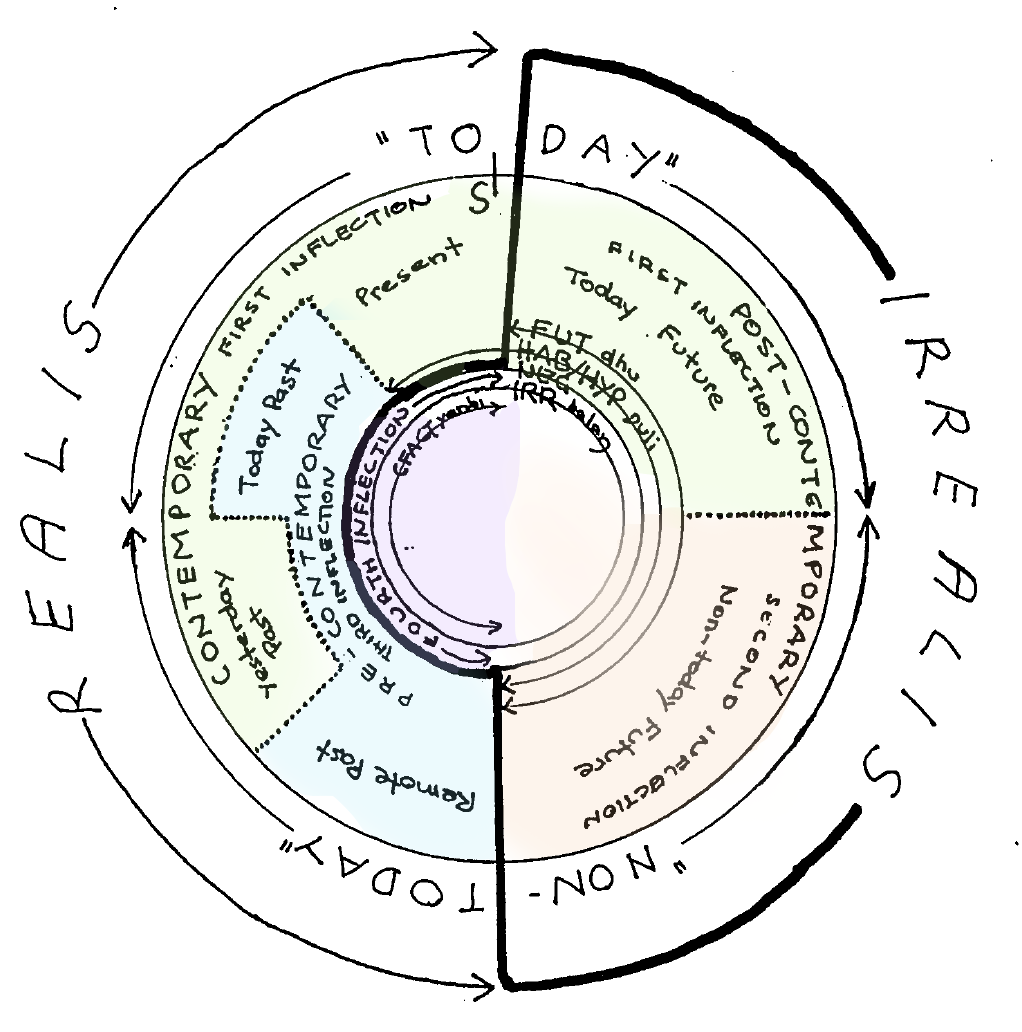
\includegraphics[width=0.85\textwidth]{WilkinsonDiagram362Col}
\end{figure}

Chapter \ref{yol-bkgd} provides background on Yolŋu Matha and the morphology of these languages' verbal paradigms, orienting the discussion around connections between temporal and modal concepts (particularly intention, prediction and futurity) and notions of relative grammatical ``prominence'' of tense, mood and aspect \citep[\textit{cf.}][]{Bhat1999}. %Subsequent chapter(s) focus on a number of morphosemantic phenomena (namely ``cyclic tense'' and ``asymmetric negation'') in the ``Western Dhuwal'' varieties of Yolŋu Matha, in view of providing an account of the semantics of the inflectional categories.



Subsequently, data further demonstrating the the expression of temporomodal distinctions and the interpretive intricacies of WD's paradigm semantics, focussing on a number of morphosemantic phenomena in Western Dhuwal(a) are provided in chapters \ref{sec:djr-temp} and \ref{sec:yol-mood} below. 

In light of these data, in chapter \ref{anY}, I propose a formal treatment of the paradigm on the basis of two semantic features: a temporal one -- \textsc{\textit{non-final instantiation}} -- and a modal one -- \textsc{\textit{metaphysical nonveridicality}}. As we will see, the notion of \textbf{branching times} ---introduced in chapter \ref{IntroCh} and deployed in the analysis of \textit{bambai} (ch. \ref{bambai.semx}) --- permits for a motivated, unified account of the ostensibly disparate sets of usage contexts that license each of \gls{wd}'s four inflectional categories. The essay concludes by considering the landscape of semantic variation across varieties of Yolŋu Matha, suggesting that the \gls{wd} system has arisen as a consequence of reanalysis and contact-induced meaning change.

\chapter{Background}\label{yol-bkgd}

\section{Grammars of TMA: the notion of ``prominence''}

In a \citeyear{Bhat1999} monograph, \citeauthor{Bhat1999} posits a typological parameter along which languages variably assign prominence to \textsc{tense, aspect \textup{or} mood}. For Bhat, determining which of these grammatical macrocategories a given language appears to assign ``prominence'' gives rise to a number of generalisations about characteristics of that language's grammar (``correlatable characteristics''). In particular, he suggests that, in a language where $ \mathcal C $ is given grammatical prominence, notions belonging to the other two categories tend to be ``viewed in terms of $ \mathcal C $'' (7).


An important consequence of this typology, in which languages can be classified and differentiated on the basis of these three broad types, is the implication that languages can ``move between them'' --- that is observable, synchronic variation across this parameter points to a history of reanalysis of, for example, temporal categories as modal ones. While Bhat does not explore this consequence of his typology in detail, he does point to observations in the grammaticalisation literature that have demonstrated ``cross-categorial change'' --- that is, situations where lexical material denoting some temporal, modal or aspectual category come to be reanalysed conveying meaning about a category in another semantic domain. Bhat suggest, for example, that the well-attested alternative grammaticalisation trajectories described by \cite{Bybee1994} (among others) and represented in Figure \ref{ta-gram} are determined by the ``prominence'' that a given language accords to either temporal or aspectual distinctions \citeyearpar[182]{Bhat1999}. Of course, this treatment to some degree begs the question. In a given pair of related languages, what is it that underpins the change from, \textit{e.g.}, perfect marking to perfective marking for $ \mathcal L_1 $ versus past-tense marking in $ \mathcal{L}_2 $?

\begin{figure}[h] \caption{Two examples of attested meaning change between the aspectual and temporal domains}\centering\label{ta-gram}

\begin{subfigure}[t]{.45\textwidth}\centering
		\begin{tikzpicture}[baseline=5pt]
		\draw  (0,0) node(pf)  {\textcolor{forest}{\textsc{perf}}};
		\draw (1.75,.5) node(pv) {\textsc{pfv}};
		\draw (1.75,-.5) node(ps)  {\textcolor{red}{\textsc{pst}}};
		\draw[thick,->] (pf) -- (ps);
		\draw[->] (pf) -- (pv);
	\end{tikzpicture}

\caption{\gls{perf} grams develop into \gls{pfv} markers (\citealp[e.g.][]{Condoravdi2014} for Indo-Aryan) or \gls{pst} markers (\citealp[e.g.][]{Schaden2012} a.o.)}
		\end{subfigure}\hfill
\begin{subfigure}[t]{.45\textwidth}\centering
		\begin{tikzpicture}[baseline=5pt]
		\draw  (0,0) node(pg)  {\textcolor{forest}{\textsc{prog}}};
		\draw (1.75,.5) node(ip) {\textsc{ipfv}};
		\draw (1.75,-.5) node(pr)  {\textcolor{red}{\textsc{pres}}};
		\draw[->] (pg) -- (ip);
		\draw[thick, ->] (pg) -- (pr);
	\end{tikzpicture}\caption{\gls{prog} grams develop into \gls{ipfv} markers (\citealp[see][]{Deo2015a}) or \gls{pres} markers (\citealp[e.g.][]{Heinrichs2002} for Neo-Aramaic)}
		\end{subfigure}
%\begin{tikzpicture}
%	content...
%\end{tikzpicture}
\end{figure}

\subsection{Futurity and mood-prominence}
Bhat marshalls data from Tibeto-Burman to show that ``mood-prominent'' languages have a tendency to grammaticalise a \textsc{future/nonfuture} distinction. He points in particularly to Manipuri ([\gls{mni}] Tibeto-Burman: Manipur), where this tense distinction appears to have ``developed from an earlier realis-irrealis modal distinction'' \citeyearpar[19]{Bhat1999}. Semantic connections between modal and future concepts are further suggested by frequently-attested semantic change pathways between, for example, expressions of intention and obligation (\textit{sc.} bouletic/deontic necessity) and futurity \citep[and then to epistemic modality, \textit{e.g.},][]{Bybee1978,Bybee1991,Bybee1994,Kuteva2019}.\footnote{\citet*{Bybee1991} hypothesise that the ``age'' of a future marker (\textsc{FutAge}) can be assessed in view of its semantic domain. In effect this amounts to a ``pathway'': $\textsc{deontic}\to\textsc{circumstantial}\to\textsc{future}\to\textsc{epistemic}$ \textit{etc.}} In her account of the diachrony (and ``instability'') of future expression in Romance, for example, \citet[31, 75, 106]{Fleischman1982} claims that as future markers become ``more temporalized'' (which she connects to their agglutination), functional pressure to recruit novel modal constructions emerges --- an early conceptualisation of a grammaticalisation cycle/``spiral.''
	%
	%The verbal suffix \textit{-le} is a future tense marker in Manipuri [\gls{mni}], whereas \citet[67ff]{Bhat1999} shows that in related Mao Naga [\gls{nbi}], it encodes irrealis modality, occurring in a number of modal, counterfactual and evidential constructions.
	%
	%\pex\a\begingl\gla \rightcomment{[Mao Naga]}alemono ovo hrü \textbf{le}-\textsc{t}i-e//
	%\glb Alemo pig buy \textbf{\gls{irr}}-\textsc{relevant}//
	%\glft`Alemo wanted to buy a pig (but couldn't as there was no money).'//\endgl
	%\a\begingl\gla pfo ico avuo bu \textbf{le}//
	%\glb he now meal take \textbf{\gls{irr}}//
	%\glft`He must be taking his meal now.'//\endgl
	%\xe


As suggested in \S~\ref{BT-review}, going back to Aristotle, it is well understood that the future has a dually temporal and modal character. That is, the truth of a future predication has frequently been analysed as changing with the passage of time --- that is ```future contingent'' statements can be neither true nor false' \citep[265]{Thomason1970}. Consequently, utterances about the future are often associated with predictive illocutionary force (this was a major theme guiding the analysis in part \textbf{\ref{bambai}}).

Consequently, contemporary formal treatments often embrace a modal semantics for ``future'' operators: one that departs from the earlier, priorian tense logic type approaches where truth is defined relative to time and --- the mirror image of \textsc{past} --- \textsc{future} is a sentential operator that serves to locate their prejacent subsequent to evaluation time.\footnote{Of course, as discussed in \S~\ref{BT-review}, Arthur Prior was crucially concerned about this asymmetry between the future and the past, over the course of his career he departing from an earlier belief in determinism and developing branching time models concerned with the indeterminate nature of the future. (\citealp[see][]{Copeland2020} and also \citealp[13]{Copley2009}).
	
	Generally speaking, on a deterministic view of the future, future morphemes can be unuderstood to universally quantify over an epistemic modal base (``possible candidates for the (preordained) future as far as I'm concerned'', \citealp[\textit{cf.}][]{Giannakidou2018}), whereas on non-deterministic views they quantify over a metaphysical modal base (``possible futures consistent with assumptions about metaphysical facts governing the world.'')} Modal accounts of future, then, often tend to take future-oriented morphology to universally quantify over a modal base. \citet[274]{Thomason1970} proposes a ``supervaluation''-based semantics for future-tensed predication as follows:\footnote{This following Copley's \citeyearpar[14]{Copley2009} conversion of \citeauthor{Thomason1970}'s account based on ``histories'' (which effectively imply sets of historical alternatives) into an equivalent one that speaks in terms of possible worlds. Thomason himself develops $ \mathcal{T\times W} $ frames in a \citeyear{Thomason1984} paper. See also \S\ref{BT-review} and \citep{Stojanovic2014} for discussion and an overview of different semantic approaches to the ``future contingents'' problem.}
\pex $ \denote[w,t]{\textsc{fut }p}=\left\{\begin{gathered}\begin{aligned} 1&\leftrightarrow &&\forall w'\big[w'\approx_t w \to\exists t' [t\prec t' \wedge p(w')(t')]\big]\\
0&\leftrightarrow &&\forall w'\big[w'\approx_t w \to\nexists t' [t\prec t' \wedge p(w')(t')]\big]
\end{aligned}\\
\text{undefined otherwise}\end{gathered}\right.
$\\[.5em]
\textsc{fut} $p$ is true if there's a time $ t' $ in the future of all metaphysical alternatives to $ w $ at $ t $ which $ p $ holds and false if there is no such time.\xe

\noindent As described earlier in this dissertation, $\cap\!\approx_t\!w $ represents the ``historical alternatives to $ w $ at $ t $'' (an equivalence class of worlds with identical histories to $ w $ up to $ t $) --- in effect equivalent to a \textit{metaphysical conversational background} (see \S~\ref{BT-review}.)


 Given how central this metaphysical assumption will be to the analysis, the approach taken by this chapter recasts this possible worlds formalism in terms of branching futures/times models. As in chapter \ref{bambai.semx}'s treatment of the distribution of \textit{bambai}, this will hopefully allow us to perspicaciously cash out the distinctions between the domains of \textsc{real} and \textsc{nonreal} eventualities. That is, a metaphysical conversational background $ \cap\!\approx_i $ will be representable by an equivalence class of branches, undivided until $ i $, that represent metaphysically possible developments of the world from $ i $.

\subsection{Negation and mood}\label{sec:asymneg}

Developing a broad cross-linguistic typology of sentential negation, \citet[208]{Miestamo2005} proposes a class of languages (\textsc{a/nonreal}) which have `grammaticalized the fact that negation belongs to the realm of the non-realized' --- that is, negative and modal operators are shown to interact formally in a number of ways. According to Miestamo, ``asymmetric negation'' phenomena are notably overrepresented in the languages of Australia (and to a lesser extinct New Guinea, driving him to describe \textsc{a/nonreal} as a ``circumpacific phenomenon'' (192, 411)). \citet[\S2.2]{Phillips2021b} provides an overview of a number of mood-based asymmetry phenomena in Australian languages.


For many languages, \textsc{a/nonreal} is manifested as the \textbf{neutralisation} of a grammatical distinction between \textsc{realis} and \textsc{irrealis} modalities in negative clauses. That is, ±\textsc{realised} is associated with a a morphosyntactic distinction in positive clauses that is not available in negative ones. Shown in the Gurrgoni (\gls{gge}, Maningrida: Arnhem) data in (\getref{sn-gvg}), a reality status distinction is morphologically realised in positive clauses (\getref{sn-gvg.rea}-\getref{sn-gvg.irr}) which is not available to its negative counterpart (\getfullref{sn-gvg.neg}), which is obligatorily irrealis-marked and ambiguous between a modal and non-modal reading. As we will see below, a similar phenomenon is exhibited in some varieties of Yolŋu Matha (notably those varieties closer to Maningrida.)


	\pex\deftagex{sn-gvg}
\textbf{Interactions between negation and mood marking in Gurrgoni} 
\iffalse	\a\begingl\glpreamble present-tensed //
\gla dji-na-ni wurrparn//
\glb 3s/3o-see-\textsc{precontemp} emu//
\glft `They didn't see an emu'//\endgl b.\quad\begingl\glpreamble neg present-tensed //
\gla galu dji-na-djirni djit-bolupu nuyu//
\glb \textsc{neg} 3s/3o-see-\textsc{irr} 3s-mother  //
\glft text//\endgl \fi

\a\begingl\glpreamble Past-tensed (nonmodal)\deftaglabel{rea}//
\gla nji-weki-\textbf{ni}//
\glb 2s-talk-\textsc{precontemp}//
\glft `You talked.'//\endgl \a\begingl\glpreamble Past-tensed (modalised)\deftaglabel{irr}//
\gla nji-weki-\textbf{yarni}//
\glb 2s-talk-\textsc{\textbf{irr1}}  //
\glft `You might have talked.'//\endgl	\a\begingl\glpreamble Negative past-tensed\deftaglabel{neg}//
\gla galu nji-weki-\textbf{yarni}//
\glb \textsc{neg} 2s-talk-\textsc{\textbf{irr1}}  //
\glft `You didn't/mightn't have talked.'\trailingcitation{(adapted from \citealp[307]{Green1995})}//\endgl


\xe



Irrealis markers are broadly taken to realise semantic operators which displace the instantiation of a given eventuality into the realm of the nonrealised. Relatedly, negative operators indicate the \textsc{nonrealised} status of some predicate.

Consequently, for languages exhibiting \textsc{a/nonreal}, irrealis and negative operators can be thought of as performing conceptually-related functions. \citep[see also][208]{Miestamo2005}.

 It is on these functional grounds that negation and mood interact; predicting parametric variation across languages.

%todo asymmetry. Muna participates (Bhat 67)


%\subsection{The semantics of a mood-based inflectional system}

\section{Yolŋu Matha}

%Class of YM was discussed in Ch..... 
%To reorient the reader.....
%Djr, Wag are related....
%could move post-defense
Yolŋu Matha is a small language family spoken in North-Eastern Arnhem Land, in the Northern Territory of Australia (map provided in \ref{map}, see also discussion in \S~\ref{sec:ecol}). The family is a subgroup of the larger Pama-Nyungan family, representing something of an enclave in Northern Australia; surrounded by a diversity of unrelated languages.

\begin{figure}[h]
	\centering\caption{Traditional language communities in Northern Australia \citep{Horton1996}.Yolŋu Matha is the gold coloured area within the square in the primary map.\\\textbf{Inset. }Northeast Arnhem land (colourised from \citealt[2]{Wilkinson1991}. Yellow shading indicates the \textit{Yolŋu Wäŋa} (homeland). Brown and green circles indicate the contemporary distribution of Yolŋu languages investigated. Purple circling indicates the neighbouring (but genetically unrelated) Maningrida language family.}	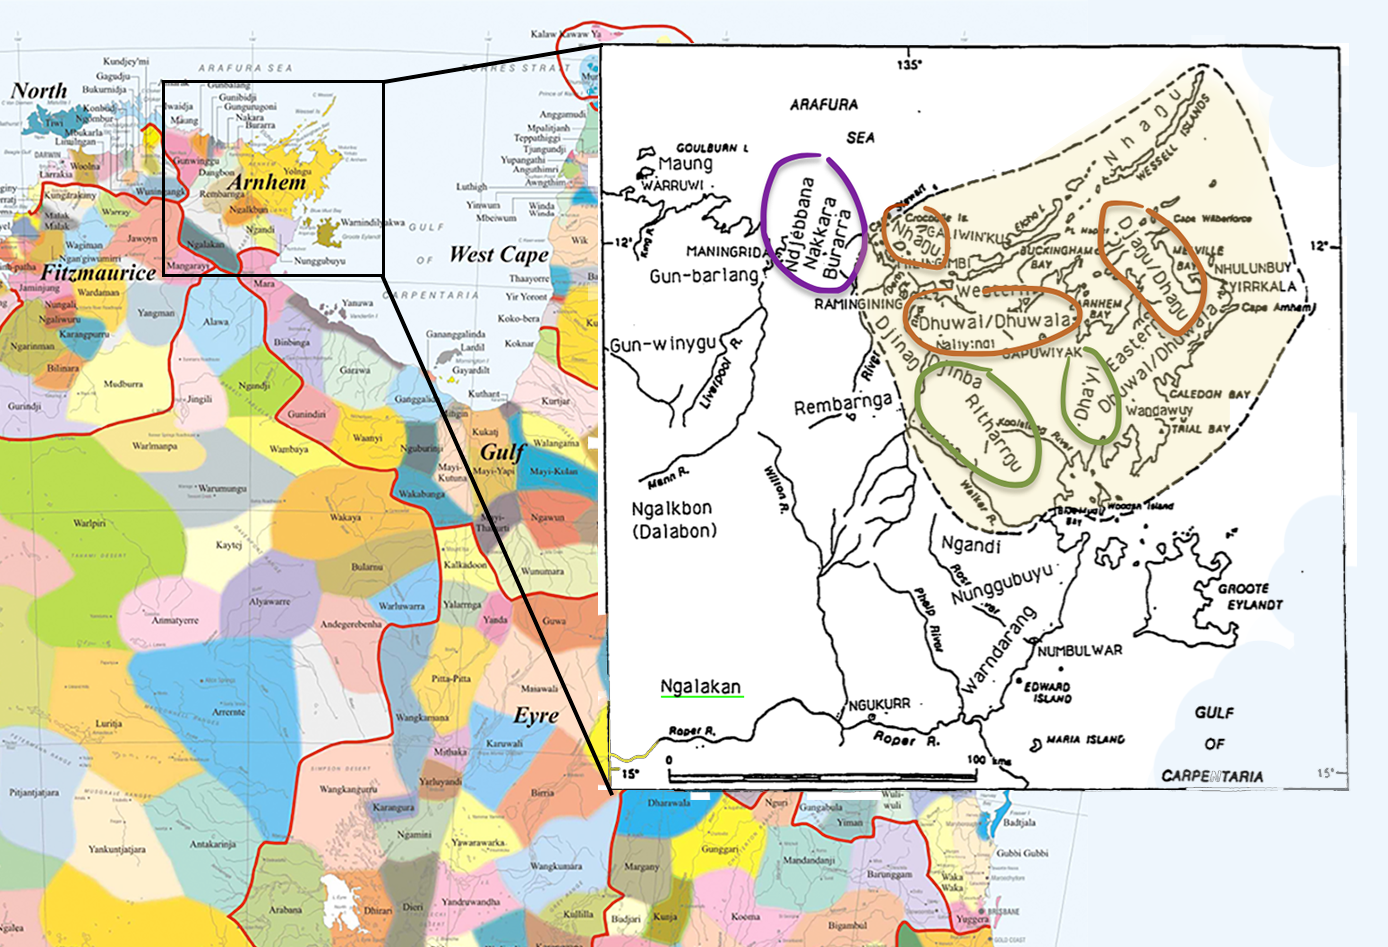
\includegraphics[width=0.9\textwidth]{AustralianLangsCropped.png}\label{map}
\end{figure}


Most Yolŋu linguistic phylogenies posit a high-level split between Western, Northern and Southern subgroups. This is schematised in Figure \ref{YM-phylo}. Yolŋu society is traditionally organised according to a moiety system --- that is, the Yolŋu universe is organised into two ranging sets, \textit{Yirritja} and \textit{Dhuwa} --- and continues to be strictly exogamous with respect to moiety. Given that each Yolŋu clan is associated with a single patrilineal moiety and corresponding language variety, households are necessarily multidialectal, one member of a couple speaking a \textit{Yirritja} lect, the other speaking a \textit{Dhuwa} lect. Children inherit their father's moiety (and language), and marry into their mother's moiety \citep[see also][62\textit{ff}]{Williams1986}. This chapter focuses primarily on a number of Southern Yolŋu varieties (see Fig \ref{DDvars}). 


\begin{figure}
\caption{A broad phylogenetic classification of Yolŋu subgroups, following \citealt{Wilkinson1991,Schebeck2001,Waters1989} a.o.}\centering\label{YM-phylo}
	\begin{tikzpicture}\tikzset{edge from parent/.style=
{draw,
edge from parent path={(\tikzparentnode.south)
-- +(0,-8pt)
-| (\tikzchildnode)}}}
		\Tree  [.\textbf{Yolngu~Matha} [.\textsc{Western} [.Djinang ] Djinba ] [.\textsc{Northern} Nhaŋu Dhaŋu-Djaŋu ] [.\textsc{Southern} \textit{Fig~\ref{DDvars}} ] ]
	\end{tikzpicture}
\end{figure}

\begin{figure}[h]\centering	\caption{Varieties (`clanlects'/dialects) of \textcolor{teal}{Dhuwal}-\textcolor{ochre}{Dhuwala} in the context of the Southern Yolŋu languages \citep[following][13]{Wilkinson1991} with some adaptation following \citet[15]{Schebeck2001}.}\label{DDvars}
	\begin{tikzpicture}[every node/.append style={align=right},every tree node/.style={anchor=north}]
		\Tree [.\textsc{\textbf{Southern~Yolŋu}} [.\textbf{\textcolor{ochre}{Ritharrŋu}-\textcolor{teal}{Wägilak}} $\vdots$ ] [ [.\textbf{Dhay'yi} $\vdots$ ] [.\textbf{Dhuwal-Dhuwala} [.\textsc{western} \node[text=teal,font=\itshape]{\bf\it Djambarrpuyŋu\\Ḻiyagalawumirr\\Ḻiyagawumirr\\Marraŋu\\$ \vdots $}; \node[font=\itshape,text=ochre]{\bf\it Gupapuyŋu\\Wubulkarra\\$ \vdots $}; ]   [.\textsc{eastern} \node[font=\itshape,text=teal] {\textbf{Djapuˀ}\\Marrakulu\\Ḏäṯiwuy\\$ \vdots $}; \node[font=\itshape,text=ochre]{\textbf{Gumatj}\\Maŋgalili\\Munyuku\\Maḏarrpa\\$ \vdots $}; ] ] ] ]
	\end{tikzpicture}
	
\end{figure}\marginnote{right this is the classification in Wilk 91 which follows Dixon 80 presumably? Claire's phylogeny is different in a number of ways. how to handle?}

As indicated in the diagram, the \textit{Dhuwal} and \textit{Dhuwala} groupings effectively represent the distinct clan-lects of a single speech community --- associated with \textit{Dhuwa} and \textit{Yirritja} moieties respectively. Incidentally, \citet{Wilkinson1991} points out that the degree of similarity between Western Dhuwal and Dhuwala are more closely related to one another than either is to Eastern Dhuwal and Dhuwala (I assume that this fact is representable phylogenetically and has been represented in Figure \ref{DDvars}). A (the?) primary distinction between Dhuwal and Dhuwala varieties cross-cutting the language area results from a productive apocope rule (investigated in \citealp{Morphy1977}, \citealp[see also][94\textit{ff}]{Wilkinson1991} for further details.). The formal consequences of Dhuwal apocope on the verbal paradigm are partially indicated in parentheses in Table \ref{djr-pdm-exx} below. The table gives examples of the verb paradigm for each of the major Djambarrpuyŋu conjugation classes as described by \citet[306\textit{ff}]{Wilkinson1991} (parentheses give the corresponding verb group number assigned by \citealt{Lowe1996} for Gupapuyŋu.)


%\section{Dhuwal-Dhuwala: Djambarrpuyŋu \& Gupapuyŋu}\label{djr}
\section{The Yolŋu verb: Typology \& morphosemantics}\label{yol-paradigms}

With the exception of the Western Yolŋu varieties \citetext{\textit{i.e.}, Djinaŋ \& Djinba, see \citealp{Schebeck2001,Waters1989}}, Yolŋu varieties are largely mutually intelligible \citep{Heath1981b,Morphy1983}. Yolŋu languages have a verbal paradigms which are at least partially cognate and likely reconstructable to a proto-system \citetext{\citealp{Schebeck2001}, \citealp[see comparative reconstruction pilot work by ][]{Bowern2009}.} All varieties have between three and six different inflectional classes; each inflection is responsible for encoding (combinations of) temporal (tense/aspect) and modal information --- as described above, it is the semantics of these inflections with which we will be primarily concerned in this dissertation. The forms of each inflection additionally varies depending on the conjugation class associated with a given verb stem (or derivational suffix) --- authors of descriptions of various Yolŋu varieties having identified between three \citetext{\citealp[\textit{e.g.},][]{Waters1989} on Djinba \& Djinba} and nine \citetext{\citealp[\textit{e.g.},][]{Lowe1996} on Gupapuyŋu} distinct conjugation classes.

In view of demonstrating the structure of a Yolŋu verbal paradigm, in this section, I present a brief overview of the morphosemantics of the range of inflectional classes in Wägilak --- the southernmost variety of Yolŋu Matha and a close relative of Dhuwal --- on the basis of new data elicited in the field, in addition to \citeauthor{Heath1980r}'s \citeyearpar{Heath1980r} description of Ritharrŋu.\footnote{Many thanks to Salome Harris for collecting questionnaire-data from Wägilak and Ritharrŋu in Ngukurr, mid-2019.}

\subsection{The Ritharrŋu-Wägilak paradigm}\label{sec:rit.paradigm}

According to \citet[60--75]{Heath1980r}, the Ritharrŋu (Wägilak) verbal paradigm distinguishes six main conjugation classes which, each of which marks four inflectional categories. These inflections establish a three-way tense distinction between the \textcolor{blue}{\textsc{past}}, \textcolor{forest}{\textsc{present}} and \textcolor{ochre}{\textsc{future}}. He describes the fourth category as the \textcolor{purple}{\textsc{past potential}}, supplying data of the latter's use in counterfactual situations. The paradigm is represented by table \ref{rit.paradigm}, while the data in (\ref{wag-infls}) demonstrates the (straightforward) temporal semantics of each of these inflectional categories.


\begin{table}[h]\caption{Examples of conjugation patterns for the Ritharrŋu-Wägilak verbal paradigm \citep[adapted from][63--6]{Heath1980r}}\label{rit.paradigm}\small
	\begin{tabular}{>{\bf}l>{\sc}l>{\it}l>{\it}l>{\it}l>{\it}l}\toprule
		\textsc{class} & \textsc{stem} & \textcolor{forest}{\gls{pres}} & \textcolor{ochre}{\gls{fut}} & \textcolor{blue}{\gls{pst}}\footnotemark & \textcolor{purple}{\gls{cfact}}\\\midrule
		1 & `go' &	wäni & wäni & wäni-\textbf{na}/-\textbf{nya} & wäni-\textbf{ya}\\
 2& `eat' & ḻuka & ḻuk-\gls{I} & ḻuka-\textbf{nha}& ḻuk\textbf{-iya}\\
 3& `chase'& ŋupa& ŋupa-\textbf{ru}&ŋupa-\textbf{na} &ŋupa-\textbf{ra} \\
 4&`hold' & gatha-\textbf{ŋ} &gaṯu-\textbf{lu} &gatha-\textbf{(la)ra} & gatha-\textbf{la} \\
 5&`push' &djaranydju\textbf{-n} &djaranydju\textbf{-ru} &djaranydju\textbf{-na} &djaranydju\textbf{-ra} \\
 6\textsc{b}&`protect' &gunga\textbf{-ma} & gungu\textbf{-ŋu}& gunga\textbf{-wala/-nha} & gunga\textbf{-wa}\\\bottomrule
	\end{tabular}
\end{table}
\footnotetext{Where there are two forms given for the \textcolor{blue}{\gls{pst}} marker, \citet{Heath} is ambivalent about the semantic characteristics of each form --- i.e., whether they are synonymous or whether they represent a defective distinction. We will provide further evidence for the latter persepctive in \S\ref{yol-change}.}



\pex \textbf{The temporal interpretation of each inflectional class in Wägilak}\label{wag-infls}
\a\begingl\gla \rightcomment{\textcolor{forest}{\textbf{[\textsc{present}]}}}\textbf{nhäma} rra yakuthi mukulnha//
\glb see.\textbf{{\I}} 1s now aunt.\textsc{acc}//
\glft`I'm (not) looking at my aunt currently.'\trailingcitation{[RN~20190520]}//\endgl\deftagex{wag-pres}\
\a\begingl\gla \rightcomment{\textcolor{ochre}{\textbf{[\textsc{future}]}}}goḏarrpuy ŋarra \textbf{nhäŋu} mukulnha//
\glb tomorrow 1s see.\II{} aunt.\textsc{acc}//
\glft`I will (not) see my aunt tomorrow.'\trailingcitation{[DW~20190522]}//\deftagex{wag-fut}\endgl
\a\begingl\gla \rightcomment{\textcolor{blue}{\textbf{[\textsc{yesterday past}]}}}ripurru-mirri ŋarra \textbf{nhäwala} mukulnha//
\glb yesterday 1s see.\textbf{\III} aunt.\textsc{acc}//
\glft`I saw (didn't see) my aunt yesterday.'\trailingcitation{[RŊ~20190522]}//\endgl\deftagex{wag-pst}
\xe

\noindent Further, (\getref{rit.mods}) shows the modal uses of \gls{fut} and \gls{cfact} inflections. In (\getfullref{rit.mods.a}-\getref{rit.mods.imp}), \II~is compatible with a number of modal (\textit{e.g.}, deontic, conditional) readings, including in imperative utterances. Similarly, \gls{cfact} is compatible with a range of ``modal-for-the-past''/counterfactual readings, as shown by Heath's translation in (\getfullref{rit.mods.cf}).


\pex \textbf{The \textsc{future} and \textsc{past potential/counterfactual} in modalised contexts in Ritharrŋu-Wägilak}\deftagex{rit.mods}
\a \begingl\gla blijiman ŋay waŋa-na: ``gulu-\textbf{rru} nhe yiŋ'-ŋiri\textdblhyphen{dhi} wäŋa-ya. Yakaŋu nhe \textbf{wäni}-'may garra nhe git lokdap-\textbf{urru}"//
\glb policeman 3s say-\III~ stay-\II~ 2s \gls{dist}-\gls{loc}\textdblhyphen\gls{foc} home-\gls{prom} \gls{neg} 2s go.\II-\gls{neg} \textit{garra} 2s \textit{get} locked.up-\II//
\glft`The policeman said you must stay here at home. Don't go (anywhere) or you'll be locked up.'\trailingcitation{[RŊ~20190520~18']}\deftaglabel{a}//\deftagex{wag-pot}\endgl
\a\begingl\gla \textbf{wäni} nhe//
\glb go.\II~ 2s//
\glft `You can/should/will go.' (or `Go!')\trailingcitation{\citep[104]{Heath1980r}}\deftaglabel{imp}//\endgl
\a\begingl\gla wäni\textbf{-ya} nhe//
\glb go-\V~ 2s//
\glft`You could/should/would/were about to go.'\trailingcitation{\citep[104]{Heath1980r}}\deftaglabel{cf}//\endgl
\xe

This distribution can be straightforwardly represented by appealing to the ``modal trichtomy'' \citetext{\textit{cf.} \citet{VonPrince2019,VonPrincea} --- introduced in \S \ref{vP-trich}, compare (\getref{trichot}), \textit{p.}~\getref{vP-bt0}.} Effectively, Ritharrŋu-Wägilak's four inflections can be thought of as a partition of a branching-time. This is shown in (\nextx) and schematised in Figure \ref{rit-BT}.


\pex \textbf{Domains of the four inflections in Ritharrŋu-Wägilak, given a branching time frame $ \mathfrak U =\langle\mathcal I,\prec\rangle$ and an evaluation index $ i* $}


\denote[i*]{\gls{pres}}  : \textsc{actual present} $ \{i\mid i = i*\} $\\
\denote[i*]{\gls{fut}}  : \textsc{potential} $ \{i\mid i \succ i*\} $\\
\denote[i*]{\gls{pst}}  : \textsc{actual past} $ \{i\mid i \prec i*\} $\\
\denote[i*]{\gls{cfact}}  : \textsc{counterfactual} $ \{i\mid \langle i,i*\rangle\text{ is unordered by }\prec\} $
\xe

\begin{figure}[h]
	\caption{Ritharrŋu-Wägilak's verbal paradigm partitions the branching frame/modal domain (modelled as a set of partially-ordered indices.)}\label{rit-BT}\centering
	\begin{tikzpicture}
		[scale=2.5,level distance=9mm,
		every node/.style={fill=purple,circle,inner sep=1.5pt},
		level 1/.style={nodes=purple,sibling distance=10mm},
		level 2/.style={sibling distance=8mm},
		level 3/.style={sibling distance=4mm},
		level 4/.style={sibling distance=2mm},
		edge from parent/.style={draw,thick}]
		\node[color=blue,minimum size=2mm] {} [grow=right]
		child {node {} edge from parent[densely dotted,color=purple]
			child {node {}
				child {node {}
					child {node {}}
					child {node {}}}
				child {node {}
					child {node {}}
					child {node {}}}}
			child {node {}
				child {node {}
					child {node {}}
					child {node {}}}
				child {node {}
					child {node {}}
					child {node {}}}}}
		child[missing]
		child {node[color=blue,minimum size=2mm] {}
			child {node {} edge from parent[densely dotted,color=purple]
				child {node {}
					child {node {}}
					child {node {}}}
				child {node {}
					child {node {}}
					child {node {}}}}
			child {node[color=purple] {} edge from parent[densely dotted,color=purple]
				child {node {}
					child {node {}}
					child {node {}}}
				child {node {}
					child {node {}}
					child {node {}}}}
			child {node [style={fill=forest,minimum size=4mm},label=above:$ \boldsymbol{{\color{gray!95}i*}} $] {} []
				child {node[fill=ochre] {} edge from parent[densely dashed,color=ochre,every child=every node\.style={fill=ochre,circle,inner sep=1.5pt}]
					child {node[fill=ochre] {}}
					child {node[fill=ochre] {}}} 
				child {node[fill=ochre] {} edge from parent[densely dashed,color=ochre]
					child {node[fill=ochre] {}}
					child {node[fill=ochre] {}}}} };
	\end{tikzpicture}
\end{figure}


As an example then, the contribution of \textcolor{forest}{\gls{pres}} (following standard assumptions about tense) is taken to be the restriction of a given predicate (\textit{P})'s instantiation to actual indices that overlap with the present: \textit{i.e.}, \gls{pres}(\textit{P}) is true iff \textit{P} is instantiated at $ i* $.

\subsection{The central Arnhem linguistic area}
This section has so far sought to familiarise the reader with the basic structure of a Yolŋu Matha verbal paradigm, taking the example of the Ritharrŋu-Wägilak (Southern Yolŋu) variety. 

In the sections that follow, we turn to a description of the distribution of the inflectional categories in Western Dhuwal-Dhuwala (\gls{wd}). As we will see (and as shown in the introduction to this part of the dissertation), there are a number of phenomena that complicate a unified treatment of the semantics of the \textsc{wd} paradigm. Introduced above, these phenomena include a \textsc{cyclic tense} system and \textsc{asymmetric negation}.


Importantly, these phenomena are not exhibited in most Yolŋu lanuages, including those varieties phyletically closest to \textsc{wd}, \textit{viz.} Ritharrŋu-Wägilak as well as the Eastern (\textit{``Miwatj''}) varieties of Dhuwal-Dhuwala centered around Yirrkala (compare figures \ref{YM-phylo} \& \ref{DDvars}.) Similar patterns are, however, characteristic of the languages of Maningrida --- Burarra, Gurrgoni, Nakkara and Ndjébanna. Varieties of Djinaŋ (a Western Yolŋu outlier) are spoken in the Maningrida community and its outstations. The Ramingining community --- traditionally the land of the Ganalbingu tribe (a \textit{Yirritja} Djinba moiety) --- is approximately 100km east of Maningrida. Djinaŋ, Djinba and \gls{wd} (the westernmost varieties of Dhuwal-Dhuwala) all exhibit the cyclicity and asymmetric negation that is characteristic of the grammars of the Maningrida languages.

In view of the sustained contact between the non-Pama-Nyungan Maningrida languages and the (geographically) western varieties of Yolŋu Matha, it is assumed here that these two properties are examples of areal phenomena that characterise the languages of central Arnhem Land \citetext{see appendix 2 of \citealt{Waters1989} for a short investigation of this perspective.}


\begin{center}
	
\huge\sf	 ※
	
\end{center}


\noindent I will argue that these two phenomena --- \textit{cyclic tense} and \textit{asymmetric negation} (w/r/t reality status marking) --- are undergirded by the grammaticalisation of two semantical properties---\textsc{\textbf{non-final instantiation}} and \textsc{\textbf{nonveridicality}} respectively. These properties will be further precised and couched in a more detailed discussion of the expression of temporal and modal categories in \gls{wd} (chh.~\ref{sec:djr-temp}--\ref{sec:yol-mood}). A formal proposal (in terms of branching times) for the semantics of the \gls{wd} verbal paradigm is presented in chapter \ref{anY}.


%todo §§4.1-4 to migrate directly in as descriptive background chapters
\section{Verbal inflection in Western Dhuwal(a)}\label{djr-infl}

%\subsection{\gls{wd} Paradigm structure \& distribution of the inflections}\label{infls}

TMA distinctions in Western Dhuwal(a) are partially encoded in a paradigm that distinguishes four `inflections', which are cognate with a number proto-Yolŋu inflections according to the reconstructions provided by \citet{Bowern2009}. Unlike for Ritharrŋu-Wägilak, summarised above (\S~\ref{yol-paradigms}), work on Dhuwal-Dhuwala varieties---most notably Beulah \citeauthor{Lowe1996}'s notes and lessons on Gupapuyŋu (first published in 1960) and Melanie \citeauthor{Wilkinson1991}'s 1991 Djambarrpuyŋu reference grammar [republished \& cited here as \citealp{Lowe1996,Wilkinson1991} respectively]---has tended to eschew a metalinguistic gloss for these inflections, given the ostensible non-unifiability of their semantics:\footnote{Relatedly, in his treatment of Djinaŋ and Djinba, \citet{Waters1980,Waters1989} glosses the function-in-context of each inflection, perhaps implying a polysemy treatment of each inflection in these languages: ``[In Djinaŋ, t]here are twelve semantic categories for every verb, which are coded by seven suffixal forms. Consequently, five of the forms each code two different semantic categories...'' \citeyear[142]{Waters1980}} the distribution of each of these inflectional categories is discussed in greater detail in this section. In addition to these inflections, the labour of encoding temporal and modal relations in \gls{wd} is shared by a (closed) class of auxiliaries, which appear to interact with the verbal paradigm. 




Further complicating the exposition of this (and a feature across Yolŋu Matha varieties, see \S~\ref{yol-paradigms}), is the fact that there are a number of \textit{conjugation (sub)classes}: \citet{Lowe1996} enumerates nine classes. The (more detailed) description by \citet{Wilkinson1991} shows that these correspond to three larger conjugation classes --- the \textit{Ø-}, \textit{N}- and \textit{Ŋ-}classes --- each associated with a number of subclasses,\footnote{\citeauthor{Wilkinson1991} identifies 14 distinct inflectional patterns in addition to a ``non-inflecting'' class \citeyearpar[307]{Wilkinson1991}.} in addition to ``non-inflecting'' and (semi-)irregular categories \citep{Wilkinson1991}. The paradigm for six \gls{wd} verbs, taken to be representative of distinct different conjugation patterns is given in Table \ref{djr-pdm-exx}.

%todo\mcom{Of course I can provide more detailed information (the subclasses) but that feels like it'd be better appended? The comparative spreadsheet i've made/Claire's 2009 stuff has most of this formative data... \\\textbf{note: Andrea Simms strongly suggests more exposition of the formal paradigm} }
\begin{table}[h]
	\caption{Examples of the paradigm of four morphological TMA inflections in Djambarrpuyŋu [\gls{djr}] and (Gupapuyŋu [\gls{guf}] resyllabification in parentheses).\\{}[\gls{djr}] data and classification from \citet{Wilkinson1991}; [\gls{guf}] data and classification from \textit{Gupapuyŋu} \citeyearpar{Lowe1996}.} \label{djr-pdm-exx}
	\centering
	\begin{tabular}{rl|>{\it}l>{\it}l>{\it}l>{\it}l}
		\textbf{Class} & \textbf{\textit{Example}} & \textup{\I} & \textup{\II} & \textup{\III} & \textup{\IV}\\\midrule
		$\boldsymbol\emptyset_{i}$\hfill(2)& \textit{marrtji} `go' & \textit{marrtji}& \textit{marrtji} & \textit{marrtji\textbf{n(a)}} & \textit{marrtji\textbf{nya}}\\
		
		$ \boldsymbol\emptyset_{\textit{a}} $\hfill (3) & \textit{ḻuka} `consume' & \textit{ḻuk\textbf{a}} & \textit{ḻuk\textbf{i}} & ḻuka\textbf{n(a)} & ḻuka\textbf{nha}\\

		$\boldsymbol\emptyset_{\textit{rr}}$ \hfill (4)& \textit{waṉḏirr(i)} `run' & \textit{waṉḏi\textbf{rr(i)}}& \textit{waṉḏi} & \textit{waṉḏi\textbf{n(a)}} & \textit{waṉḏi\textbf{nya}}\\
		
		
		
		\textbf{N}\hfill(5)& \textit{ḻupthun} `wash' &\textit{ḻuphtu\textbf{n}} & \textit{ḻupthu\textbf{rr(u)}} & \textit{ḻupthu\textbf{rr(una)}} & \textit{ḻupthu\textbf{na}}\\
		
		\textbf{N$ _{L} $}\hfill(6)& \textit{gurrupan} `give' & \textit{gurrup\textbf{an}} & gurrupu\textbf{l(u)}&gurrupa\textbf{ra}& gurrupa\textbf{na} \\
		
		\textbf{Ŋ}\hfill(7)& \textit{nhäma} `see' & \textit{nhä\textbf{ma}} & \textit{nhä\textbf{ŋu}} & \textit{nhä\textbf{ŋal(a)}} & \textit{nhä\textbf{nha}}\\
	\end{tabular}
	
\end{table}


Above, I alluded to Beulah Lowe's eschewal of a ``semantic description'' for each of the four inflectional classes, also followed by Melanie Wilkinson. Throughout, these categories will be glossed with bold-faced Roman numerals, following the conventions established by Lowe (see also Table \ref{Infl-Comparisons-Wilk}, which adapts Wilkinson's summary of glossing decisions made by other grammarians.)% -- complex sentences and predications are investigated in further detail in §\ref{djr-subord}.

%Table \ref{Infl-Comparisons-Wilk}, adapted from \citet[336]{Wilkinson1991} summarises the metalanguage decisions made by other authors in their attempts to describe Dhuwal(a) varieties.

\begin{table}[h]
	\caption{Summary of metalinguistic descriptors deployed by a number of grammarians for the four inflectional classes in a number of Dhuwal/Dhuwala varities, adapted from \citet[336]{Wilkinson1991}.}\label{Infl-Comparisons-Wilk}\small
	\begin{tabular}{lr|llll}
		&&	\textbf{\I}	& \textbf{\II}	&	\textbf{\III}	&	\textbf{\IV}\\\midrule
		\citealt{Wilkinson1991}& \gls{djr} &\textsc{First}&\textsc{Second}&\textsc{Third}&\textsc{Fourth}\\
		\citealt{Lowe1996}\footnotemark &\gls{guf} &Primary&Secondary&Tertiary&Quartenary\\
		\citealt{Tchekhoff1983}& \gls{djr}&\textsc{Bas}e&\textsc{Fut}ure&Past\textsubscript1&Past\textsubscript2\\
		\citealt{Heath1980}& \gls{dwu} & Pres/Fut & Fut/Imp & Past & Past Remote\\
		\citealt{Morphy1983}& \footnotesize Djapuˀ & Unmarked & Potential & Perfective & Past Non-indicative\\
	\end{tabular}
	
\end{table}	\footnotetext{\Citealt{VanderWal1992} adopts the same labelling scheme as \citet{Lowe1996} although her analysis of the distribution of each of Gupapuyŋu's inflectional classes seems to diverge somewhat from \citeauthor{Lowe1996}'s.}

 In the following subsections, I provide examples of the functional domains of each of the four inflections in Western Dhuwal-Dhuwala and other lexical material relevant to encoding TMA relations in this language.

%todo MW diagram is now in the intro to this subpart
% Figure \ref{WilkDia} comprises a (colourised) reproduction of \citeauthor{Wilkinson1991}'s schematisation of the functional domain and collocation features of each Djambarrpuyŋu inflection. Data exemplifying the distribution of WD's four inflectional categories is provided in the subsections below in conjunction with a discussion of the approximate range of each.
%
%\begin{figure}[h]\caption{Melanie Wilkinson's \citeyearpar[326]{Wilkinson1991} schematisation of the complex semantic space associated with each of the four inflectional categories in Djambarrpuyŋu. My colourisation.}\label{WilkDia}\centering
%	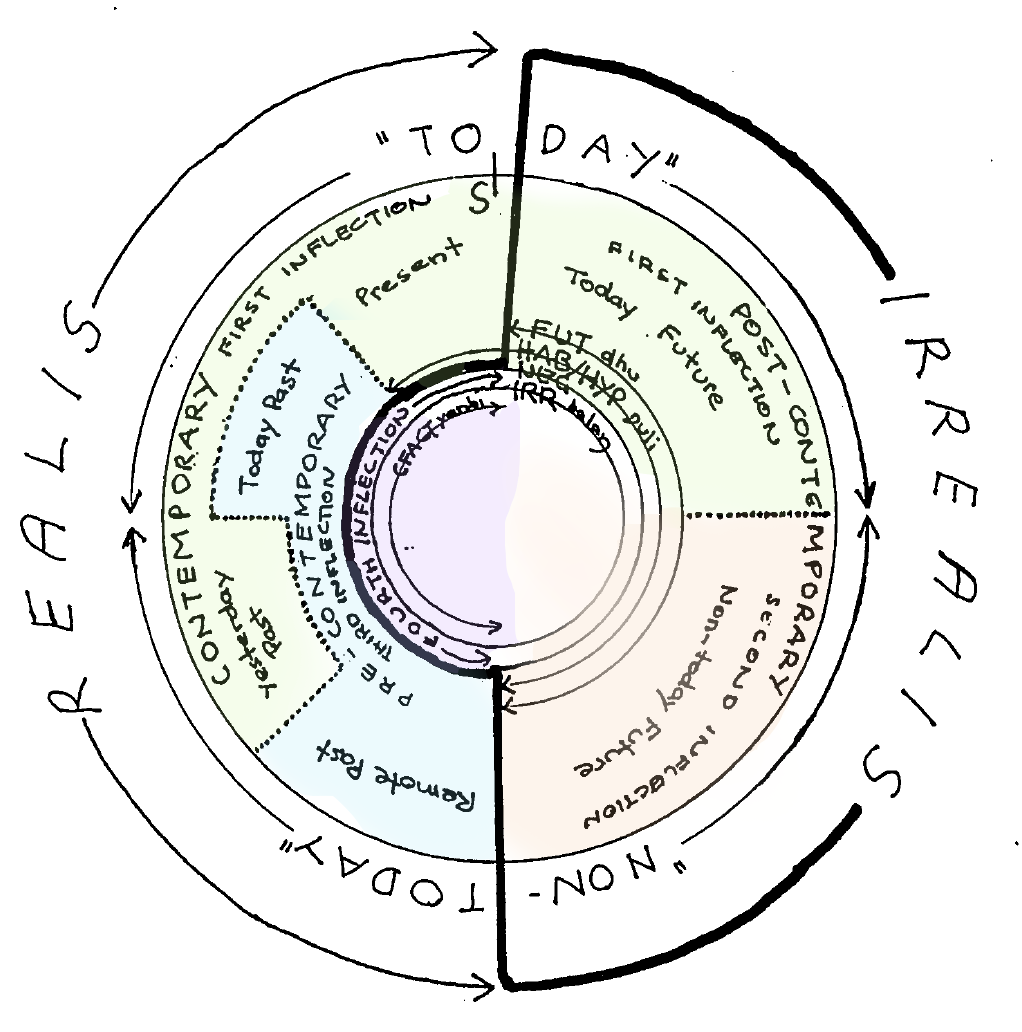
\includegraphics[width=0.8\textwidth]{WilkinsonDiagram362Col}
%\end{figure}

\subsection{The Primary inflection}\label{desc-i}

The `primary' inflection (\I), cognate with inflections in other Yolŋu languages which have been described as ``unmarked'' or ``base'', surfaces in predications that are interpreted with any of \textsc{present}, \textsc{past} or \textsc{future} reference. Here I provide examples of \I-inflected clauses receiving each of these temporal interpretations.

%\mcom{Now for both of these (and i suspect all sentences in this sssection) context ought to be modulable s.t. a non-present reading is available. This can/should/will be tested in the field}
\pex\textit{\textbf{ Present-reference encoded with \gls{I}}}

\a\begingl\deftagex{IPres}\deftaglabel{nhina}
\gla Ŋunhi-y ŋunhi ḏirramu \textbf{nhina} ga//
\glb \gls{texd}\textsc{-erg} \textsc{texd} man sit.\I{} \textsc{ipfv.\I}//
\glft`There that man is sitting.'\trailingcitation{\citep[856]{Tchekhoff1983}}// 
\endgl
%\a\begingl \gla ŋarra \textbf{marrtji}-n dhiyaŋu-n bala//
%\glb 1s go\textbf{.I}-\gls{seq} \gls{prox}.\gls{erg}-\textsc{seq} then//
%\glft`I am going now.'\trailingcitation{\citep[256]{Wilkinson1991}}//\endgl
\a\begingl\gla Ŋarra ga \textbf{ḻuka} gapu (dhiyaŋu bala)//
\glb 1s \textsc{ipfv.\gls{I}} consume.\gls{I} water \gls{texd}.\gls{erg} then//
\glft`I'm drinking water at the moment.'\trailingcitation{[DhG 20190405]}//\endgl
\xe

The sentences given in (\getref{IPres}) show the compatibility between present temporal reference and the \gls{I} inflection: in both cases, the event described by the predicate --- \textit{nhina} `sit.\gls{I}' and \textit{marrtji} `go.\gls{I}' --- is understood as contemporaneous with speech time. In each sentence, imperfective marking (\textit{ga} `\gls{ipfv}') is obligatory in order to establish present reference (see \S \ref{sec:djr-temp}).



In addition to those present-referring sentences in (\getref{IPres}), the data in (\getfullref{pstI}) show compatibility between \gls{I} and past time reference. In each of these examples, the events described by the predicates---\textit{e.g.}, the arrival event described by \textit{ŋayatham} in (\getfullref{pstI.ŋayatham})---\textit{precede} speech time. Similarly, the two past events in (\getref{pstI.rrupiya}) both receive \gls{I} inflection. The instantiation times of both of these events are further restricted (to the recent past) by temporal frame adverbs \textit{barpuru} $\approx$ `yesterday'. % -- frame adverbials of this type are discussed in some detail in §\ref{TFA}.

%\mcom{Is it a shitty idea to use colour coding for more formatting/highlighting options? I want to reserve bold for the verbforms themselves but would like to be able to second-order emphasise non-paradigmatic things like TFAs, aspectual ops...}
\pex\textbf{Past-reference encoded with \gls{I}}\deftagex{pstI}

%\a\deftaglabel{nhama}\begingl\gla barpuru linyu \textbf{nhäma} dirramu-ny//
%\glb yesterday 2d see.\gls{I} boy-\gls{acc}//
%\glft`Yesterday we saw a boy'\trailingcitation{\citep[569]{Tchekhoff1985}}//\endgl

\a\begingl\gla bäru-yi-\textbf{rri} \textbf{barpuru} nhuma-laŋgu rra ŋunhi-li-yi ga ŋäṉḏi-w ŋarra \textbf{barpuru} ḻarr-\textbf{uma} ga nhuma rraku ḻakara-\textbf{ma}\deftaglabel{baru}//
\glb crocodile-\gls{inch}-\gls{I} \textbf{yesterday} 2p-\gls{dat} 1s \gls{texd}-\gls{loc}-\gls{ana} and \gls{mo}-\gls{dat} 1s \textbf{yesterday} search.for-\gls{I} and 2p 1s.\gls{dat} tell-\gls{I}//
\glft`Yesterday, I (appeared) to you as a crocodile there. And I was looking for my mum and you told me (where she was.)'\trailingcitation{\citep[107]{VanderWal1992}}//\endgl

\a\deftaglabel{ŋayatham}\begingl\gla ga \textbf{ŋayatham} ŋunha baṉ'thula-wuy ŋayambalk//
\glb and reach.\gls{I} \gls{dist} \textsc{place}-\gls{assoc} place//
\glft`And (then we) reached the place (associated with) Baṉthula.'\trailingcitation{\citep[461]{Wilkinson1991}}//\endgl



\a\deftaglabel{rrupiya}\begingl\gla ḏirramu-wal yothu-wal bäpa-'mirriŋu-y rrupiya \textbf{barpuru} djuy'yu-\textbf{n} märr \textbf{barpuru} ga \textbf{barpuru} \textbf{buna}-ny dhiyal-nydja//
\glb man-\gls{obl} kid-\gls{obl} father-\gls{kinprop}-\textsc{erg} money \textbf{yesterday} send-\gls{I} \textbf{somewhat} \textbf{yesterday} and \textbf{yesterday} arrive.\gls{I}-\textsc{prom} \gls{prox}.\gls{erg}-\gls{prom}//
\glft`The father sent money to the boy recently and it arrived here yesterday'\trailingcitation{\citep[343]{Wilkinson1991}}//\endgl

\xe


Finally, the examples in (\getref{futI}) below, show the compatibility of \gls{I}-inflected verb forms and \textsc{future} temporal reference.  In these contexts, the presence of \textit{dhu} --- the \textsc{future} marker (to receive a modal semantics) --- is obligatory in order to establish future reference. 

\pex \deftagex{futI} \textit{\textbf{Future-reference encoded with \gls{I}}}
\a\deftaglabel{lakaram}\begingl\gla yalala ŋarra dhu nhokal lakara-\textbf{m}//
\glb later 1s \textsc{fut} 2s\textsc{.obl} tell-\gls{I}//
\glft `Later (today) I'll tell you.' \trailingcitation{\citep[373]{Wilkinson1991}}//\endgl

\a\deftaglabel{buna}\begingl \gla dhiyaŋ~bala walal dhu \textbf{buna}, yalala//
\glb now 3p \textsc{fut} arrive.\gls{I} later//
\glft`They are coming later today.'\trailingcitation{\citep[256]{Wilkinson1991}}//\endgl


\a\begingl\glpreamble \textbf{Deontic force with \textit{dhu}+\gls{I}}//
\gla Way! Nhe dhu gurruka-\textbf{m} helmet! Rom ga \textbf{waŋa}.//
\glb Hey! 2s \gls{fut} wear-\gls{I} \textit{helmet} law \textsc{ipfv.\gls{I}}  say.\gls{I}//
\glft`Oy! You wear a helmet! The law says so!\trailingcitation{[AW~20170730]}//\endgl

%\a\deftaglabel{marrtji}\mcom{Actually, W claims this is ``imminent action'' so we really just have a futurate use of \gls{I} without \textit{dhu} (interesting data point in itself) This can probably move to the section on future marking (either \gls{I} or \textbf{\textit{dhu}})}\begingl\glpreamble `Imminent action' without \textit{dhu}//
%\gla \ljudge{$ ^{\%*} $}ŋarra marrtji-n \textbf{dhiyaŋu}-n \textbf{bala}//
%\glb 1s go-\gls{seq} \textbf{\gls{prox}.\gls{erg}}-\gls{seq} \textbf{\gls{mvtawy}}//
%\glft`I'm going now.'\trailingcitation{\citep[256]{Wilkinson1991}}//\endgl

\xe


\noindent In each of these three sentences, the event described by the predicate is understood to obtain in the \underline{future} of speech time (modulo additional constraints on imminence/immediacy, to be described in the next subsection.)

What we have seen here, then, is that \gls{I} is compatible with temporal reference at, prior to, and subsequent to the moment of speech: on the basis of this evidence, we might conjecture that it has no temporal semantics. %\mcom{Evidence of infelicity of \textit{dhu}-less future readings? I actually kinda doubt on the basis of Tonnhauser, Bohnemeyer's work that this is going to be a hard constraint}
%(Although according to \citet[256]{Wilkinson1991} (\getfullref{futI.marrtji}), a futurate interpretation is ostensibly available. This use is unavailable to Ramingining speakers.

\subsection{The Secondary inflection}\label{desc-ii}

Like \gls{I}, the Secondary inflection (\gls{II}) has a range of uses. It is notably obligatory when predicating of future times \underline{beyond the current day} and is the main strategy for forming \underline{imperative sentences}.

\pex\deftagex{futII} \textbf{\textit{Future-reference encoded with \gls{II}}}
\a\deftaglabel{lakaraŋ}\begingl\glpreamble \textbf{Co-occurring with \textit{dhu} `\gls{fut}'}//
\gla yalala-ŋu-mirri-y ŋula~nhätha ŋarra *(dhu) nhokal lakara\textbf{-ŋ}//
\glb later-\textit{ŋu}-\gls{prop}-\gls{erg} sometime 1s \textsc{fut} 2s-\gls{obl} tell-\gls{II}//
\glft`I'll tell you sometime later on'\trailingcitation{(\citealp[346]{Wilkinson1991}; neg. judg. -- DhG~20190405)}//
\endgl

\a\begingl\glpreamble\textbf{ Infelicity of \gls{I} with non-today future}//
\gla Barpuru goḏarr ŋarra dhu nhä(\textbf{-ŋu/$^\#$-ma})//
\glb funeral tomorrow 1s \gls{fut} see(-\gls{II}/$^\#$-\gls{I})//
\glft `I'll see the funeral tomorrow'\trailingcitation{[AW~20180730]}//\endgl

\a\begingl\glpreamble\textbf{\textit{dhu}+\gls{I} implies same-day future}//
\gla walal $^\#$(dhu) \textbf{buna} yalala//
\glb 3p $^\#$(\gls{fut}) arrive.\gls{I} later//
\glft`They'll arrive later.'\\
\textsc{\textbf{speaker comment:}} You're talking about \textit{yalala}; not tomorrow, sometime today.//\endgl


\xe

\noindent The two sentences in (\getref{futII}) show how \gls{II} is used in concert with the particle \textit{dhu} to establish future temporal reference.
% The conditions on the (non-)appearance of \textsc{fut}-marker \textit{dhu} are unclear at the present time (see §\ref{dhu} for more), but future-readings with \gls{II} do not appear to be reliant on this auxiliary (cf. the data in (\getref{futI}) above).
  A notable contrast between (\getfullref{futI.lakaram}) and (\getfullref{futII.lakaraŋ}) is the apparently obligatory retrieval of a \textsc{today}-reference time for \gls{I}-inflected futures, as against a  \textsc{beyond-today}-reference time for \gls{II}-inflected futures.\footnote{\citet[347]{Wilkinson1991} gives an example of a speaker using a \textit{dhu}-\gls{II} structure in the context of a narrative she is telling, signalling that she `will (return to the time of the old people).' Wilkinson takes this as evidence of an association between \gls{II} and the irrealis. This generalisation is pursued in detail in this chapter.} Effectively, this distinction seems to be one place where the grammar of Dhuwal(a) grammaticalises ``temporal remoteness'' (\citealt{Comrie1985,Dahl1985} referred to elsewhere in the literature as ``metrical tense'' \citealp[\textit{e.g.},][204]{Chung}).\footnote{Although \citet[39]{Heath1980} suggests of the \gls{II} future in Dhuwal Proper (his \textsc{Fut/Imp}) that this form encodes a type of ``normative nuance'' (a clear extention of imperative flavour into future assertions.)}


(\getref{irrII}) shows the compatibility of \gls{II} with a (future-oriented) possibility reading. Modal particles including \textit{balaŋ(u), ŋuli} and \textit{bäynha} are responsible for the `weakening' or `downtowning' of the speaker's commitment to the prejacent proposition. 
%Modal operators are described in §\ref{modals}.

%\mcom{It would be good to get sentences with richer context (i.e. an established time of instantiation for the prejacent (tomorrow, imminently etc...)) 
%	This said we can probably assume that the we're talking about immediate future here... Is \gls{I} incompatible with this? There's not much more to say here until I have speaker judgments on this question.}
\pex\textbf{Future possibilities marked with \gls{II}}
\a\deftagex{irrII}\begingl\gla Ŋarra ŋuli \textbf{bäynha} dhiŋgu-\textbf{ŋ} ŋawulul-yu//
\glb 1s \textsc{hyp} \gls{mod} die-\gls{II} smoke-\textsc{erg}//
\glft`I might die from the smoke.'\trailingcitation{\citep[164]{Buchanan1978}}//\endgl
\a\begingl\gla ŋayi bala \textbf{balaŋu} bukthu-\textbf{rru}//
\glb 3s \gls{mvtawy} \gls{mod} break-\gls{II}//
\glft`It (the recorder) might break.'\trailingcitation{[DhG~20190417]}//\endgl
\xe



\gls{II} is additionally used to encode imperative clauses (\getref{impII}). Shown in (\getfullref{impII.proh}), negative imperatives (probibitives) are treated identically.\footnote{Although, as discussed in Ch. \ref{NEC} (see also \citeauthor{Phillips2021b} ms. `Negation (in Australian Languages)'), the use of privative-marked nominals is another common, more ``indirect'' directive convention.}

\pex\textit{\textbf{Imperative force with \gls{II}}}\deftagex{impII}
%\a\begingl\gla g...y, ḻupmara-\textbf{ŋu}-n ŋarra-ny//
%\glb \textsc{name} wash-\gls{II}-\gls{seq} 1s-\gls{prom}//
%\glft`G...y, wash me!'\trailingcitation{\citep[360]{Wilkinson1991}}//\endgl

\a\begingl\gla wäy! gurtha ŋunha, nhawi, ḏutji män-\textbf{ŋu}, bakmara-\textbf{ŋu}//
\glb hey! fire(wood) \gls{dist} what's.it firesticks get-\gls{II} break\textbf{-II}//
\glft`Hey! Get that firewood, what's it, those firesticks, and break them.'\trailingcitation{\cite[114]{VanderWal1992}}//\endgl

\a\deftaglabel{proh}\begingl\gla yaka walala-ŋ buku-bakamara-\textbf{ŋ}//
\glb \gls{neg} 3p-\gls{dat} head-break-\gls{II}//
\glft `Don't answer them!'\trailingcitation{\citep[360]{Wilkinson1991}}//\endgl


\a\begingl\gla nhä\textbf{-ŋu} nhanŋu dhurrwara!//
\glb look-\gls{II} 2s.\gls{dat} door//
\glft`Look at her mouth!'\trailingcitation[AW 20180731]//\endgl

\xe

Here, \II-marked predicates have been shown to be compatible with \textbf{future} temporal reference. They co-occur with \textit{dhu} (which we analyse as a \textsc{future} particle) to establish instantiation of the predicate subsequently to the day of utterance. \II~also occurs in imperative utterances and in (future-oriented) modal constructions with present perspective (\getref{irrII}).


\subsection{The Tertiary inflection}\label{desc-iii}

The Tertiary inflection (\gls{III}) is generally associated with predications about the \textsc{past}. An important caveat, however, is that this inflection is \ul{infelicitous when describing \textsc{recent} events instantiated \textsc{before the current day}.} The examples in (\nextx) below show the compatibility between \gls{III} and a reference time that is `earlier today. In (\getfullref{pstIII.rp}-\getref{pstIII.sdp}), apparent complementary distribution between \gls{I} and \gls{III} provides evidence of the categoricity of this distribuitional constraint.

\pex \textbf{\textsc{Today past} and the \gls{III} inflection}\deftagex{pstIII}


\a\deftaglabel{gathur}\begingl\gla Gäthur ŋayi \textbf{marrtjin} räli Galiwin'ku-ŋur//
\glb today 3s go.\gls{III} hither \textsc{place}-\gls{abl}//
\glft`[Earlier] today he came from Galiwin'ku.'\trailingcitation{\citep[150]{Buchanan1978}}//\endgl

\a\deftaglabel{bili}\begingl\gla Bili ŋayi \textbf{marrtjin} dhipuŋur natha-ŋur nyan'thuna-ŋur//
\glb \textsc{compl} 3s go.\gls{III} \textsc{prox.abl} food-\gls{abl} eat.\gls{IV}-\textsc{abl}//
\glft`He's already gone from having lunch here.'\trailingcitation{\citep[150]{Buchanan1978}}//\endgl

\a\begingl\gla dhiyaŋu~bili goḏarr'mirri ga-\textbf{na} dhärra-\textbf{na} märrma' malwan, bala ŋayi Ŋarritjnydja wurrth-\textbf{urruna}.//
\glb \gls{prox}.\gls{erg}~\gls{cplv} morning.\gls{prop} \gls{ipfv}-\gls{III} stand-\gls{III} two \textit{sp.~Malvaceae} \gls{mvtawy} 3s \gls{malk}.\gls{prom} pull-\gls{III}//
\glft`Earlier this morning, there were two trees standing [there], then Ŋarritj pulled them up.'\trailingcitation{[DB~20190405]}//\endgl

\a\begingl\glpreamble \textbf{Infelicity of \gls{III} with \textsc{recent past}\deftaglabel{rp}}//
\gla barpuru ŋarra nhä\textbf{(-ma/*-ŋala)} ḏetuŋ//
\glb yesterday 1s see\textbf{(-\gls{I}/$^\#$-\gls{III})} buffalo//
\glft`I saw a buffalo yesterday.'\trailingcitation[MD 20180802]//\endgl

\a\begingl\glpreamble\textbf{ Infelctity of \gls{I} with \textsc{today past}}\deftaglabel{sdp}//
\gla gathura ŋarra nhä\textbf{($^\#$-ma/-ŋala)} ḏetuŋ dhukarra-ŋura//
\glb today 1s see\textbf{$ ^\# $-\gls{I}/\gls{III}} buffalo road-\gls{loc}//
\glft `I saw a buffalo down the road today'\trailingcitation{[MD 20180802]}//
%\textsc{comment.} Event could have happened this morning or ten minutes before speech time.//\
\endgl
\xe

%todo ??unsure what this means?? \mcom{Potentially look for a ref for this or provide data that makes this unambiguous...}
\noindent(\getfullref{pstIII.gathur}) shows the compatibility between temporal frame adverbial (TFA) \textit{gäthur(a)} `today' and \gls{III} in \gls{djr}, which leads to an temporal interpretation of `earlier today.'\footnote{Note however that the reckoning of \gls{tfa} \textit{gäthur(a)} differs to that of English and other familiar languages as shown in (\getfullref{neg-pst.munha}), where \textit{gäthur munhawa} `today nighttime' is interpreted as ``last night'' and still triggers \gls{III} marking on the verb.} However even in the absence of a \gls{TFA}, the event described in (\getref{pstIII.bili}) is interpreted as having been instantiated \textsc{earlier.today}/in the immediate past of speech time. Nonetheless, as the data in (\nextx) show, a description of \gls{III} as `hodiernal/same-day past' tense marker is inadequate.


\pex\textbf{\textsc{Remote past} and the \gls{III} inflection}\deftagex{remIII}

%\a\deftaglabel{wawa}\begingl\gla nhä nho-kiyin-gal wäwa-'mirriŋu-y warkthu-\textbf{rr} ŋäthil rarrandharr-yu//
%\glb what 2s-\textsc{emph}-\gls{obl} bro-\gls{kinprop}-\gls{erg} work-\gls{III} before dry~season-\gls{erg}//
%\glft`What did your brother do last summer?'\trailingcitation{\citep[343]{Wilkinson1991}}//\endgl

\a\begingl\glpreamble\textsc{context.} A dreamtime myth.\deftaglabel{baru}//
\gla bäru ga-\textbf{na} marrtji-\textbf{na} beŋuru Ḏulkarri'garri-ŋuru//
\glb crocodile \gls{ipfv}-\gls{III} go-\gls{III} \gls{indef}.\gls{abl} \textsc{place}-\gls{abl}//
\glft`The crocodiles came from Ḏulkarri'garri.'\trailingcitation{\Citep[111]{VanderWal1992}}//\endgl

\a\deftaglabel{sydney}\begingl\gla (Ŋathili) ŋarra marrtji-\textbf{na} Sydney-lili//
\glb before 1s go-\gls{III} Sydney-\gls{all}//
\glft`I went to Sydney long ago.'\trailingcitation{[DhG~20190504]}//\endgl

\a\deftaglabel{malwan}\begingl\glpreamble\textsc{context.} The speaker is describing a locality as it was in her youth.//
\gla märrma' ga-\textbf{n} malwan-dja dhärra-\textbf{n} yindi maṉḍa-ny//
\glb two \textsc{ipfv}-\gls{III} hibiscus-\gls{prom} stand-\gls{III} big 3d-\gls{prom}//
\glft`Two big hibiscus flowers were (growing).'\trailingcitation{\citep[339]{Wilkinson1991}}//\endgl



%todo heath  dhuwal -- unexpected I --- this is a nice datapoint, but it's unclear and it's also on whatever variety H was working on.

%\a\deftaglabel{wuŋgan}\begingl\glpreamble\textsc{context.} A man is telling a story from long ago . His friend's dog has spotted a water goanna.//
%\gla ...ŋunhi wurkaḏi-y nhä-\textbf{ŋal}-{na} ŋinya dharpa-lil-a ŋal'yu-\textbf{na} nhäwi wan'kawu-ya//
%\glb \gls{texd} \textsc{name}-\gls{erg} see-\gls{III}-\gls{seq} 3s.\gls{acc} tree-\gls{all}-\gls{seq} ascend-\gls{III} whatsit water.goanna-\gls{ana}//
%\glft`\textit{Wukaḏi} watched it scramble up into a tree, the water goanna.'\trailingcitation{\citep[193]{Heath1980}}//\endgl
%todo >>>>> \marginnote{I've taken some liberties with the glossing here, Heath has the second verb \textit{ŋal'yuna} as \gls{I} with a \textsc{seq} marker... to investigate further perhaps}



\xe


Unlike the \textsc{hodiernal} temporal interpretations that the sentences in (\blastx) receive, the sentences in (\lastx) involve reference to the `\textsc{remote past}.' In (\getfullref{remIII.baru}-\getref{remIII.sydney}),%\mcom{may be easier just to get a similar non-interrogative sentence to do what \lastx b does}
 the instantiation time of the predicate is restricted by frame adverbials: \textit{ŋäthil(i)}, which picks out a time `in the distant past; prior to/earlier than (some other time)' \citep[158]{Wilkinson1991}, in addition to and \textit{rarrandharryu} `dry season':\footnote{The suffix \textit{-Thu} (\textit{-yu} as a postsonorant allomorph), glossed here as \gls{erg} is used to mark ergative NPs as well as instrumental (\gls{instr}) NPs and to form TFAs out of nominals \gls{temp}.} The cooccurrence of these expressions restricts the predicate being questioned to \textit{a prior dry season}. Conversely, the declarative sentence in (\getfullref{remIII.malwan}) requires no adverbial specification. A \textsc{remote past} interpretation arises as a result of the \gls{III} inflection alone, which is precised pragmatically by the discourse context (\textit{sc.} a narrative that the speaker is telling about her childhood.) (\getref{remIII.malwan}) will be able to retrieve a same-day past interpretation as well, with sufficient contextual support.

%\mcom{This discussion of the Maningrida treatments of ``frame'' and ``tense'' may be better placed • entirely in the lit. review, • after the general data discussion of inflections, or • in the following chapter.} 
The ostensible `discontinuity' of the times that predicates receiving \gls{I} and \gls{III} inflection can refer to has been described in preceding literature as \textbf{\textsc{cyclic time reference}} \citep[88]{Comrie1983}. In her treatment of Burarra [\gls{bvr}], \citet{Glasgow1964} draws a distinction between `tense' and `frame of reference' (`timescale' for \citealt[48]{Green1987}). These, in effect, amount to categorical interpretive interactions between morphological marking and sets of contexts. The interaction between these can be understood as giving rise to a reference interval. This style of analysis has been adopted and developed by others working on Maningrida languages \citetext{\citealt[165]{Eather2011} for Nakkara [\gls{nck}], \citet{Green1995} for Gurr-goni [\gls{gge}] and \citet{McKay2000} for Ndjébanna [\gls{djj}].} The interpretation of interacting ``tense'' morphology and reference frames is schematised in Table \ref{GlaswegianTR}. 
%todo The following chapter further treats and formalises this analysis.



\begin{table}[h]\centering\onehalfspacing
		\caption{A \citealt{Glasgow1964}-style analysis of \textbf{past-time restrictions} introduced by the verbal inflections, adapted for the Dhuwal(a) data. \gls{I} and \gls{III} inflections correspond to Eather's \textbf{contemporary} and \textbf{precontemporary} ``tenses'' (``precontemporary'' is Eather's \citeyearpar[166]{Eather2011} relabelling of Glasgow's ``remote'' tense.)}\label{GlaswegianTR}
	\begin{tabular}{@{}llll@{}}\toprule
		
		&                 & \multicolumn{2}{c}{\textsc{frame}}          \\ 
		&                 & \multicolumn{1}{c}{\textbf{today}}         & \multicolumn{1}{c}{\textbf{before today}}      \\\midrule
		\multirow{2}{*}{\textsc{\rotatebox[origin=c]{90}{infl}}} & \textbf{\phantom{\gls{I}}\gls{I}}    & now           & yesterday/recently \\
		& \gls{III} & earlier today & long ago           \\ \bottomrule%(l){2-4} 
	\end{tabular}
\end{table}


Additionally, there exists a set of psychological predicates that are frequently translated into English as present-tensed stative verbs which also (obligatorily) appear with \textbf{III}. Examples are given in (\nextx).


\pex\deftagex{psychPreds}\textbf{Apparent present reference with \gls{III}}\a\begingl\gla ŋarra dhuwal/dhika djawaryu-\textbf{rr}/rerrikthu-\textbf{rr}/djanŋarrthi-\textbf{n}//
\glb 1s \textsc{prox/indefp} be.tired-\gls{III}/be.sick-\gls{III}/be.hungry-\gls{III}//
\glft`I'm (a bit) tired/sick/hungry'\trailingcitation{\citep[278]{Wilkinson1991}}//\endgl
\a\begingl\gla bili djawar'yu-\textbf{rr}-a//
\glb \gls{cplv} be.tired-\gls{III}//
\glft`They're already tired'\trailingcitation{\citep[365]{Wilkinson1991}}//\endgl
%todo \mcom{Needs elicitation work, appears to be a today-past thing? Are these predicates available with TFAs \textit{barpuru?}, with \textit{ga}? And the other inflections??\\	Test entailments also: \textit{??I was tired this morning but i'm not now??}}
\a\deftaglabel{nhaŋal}\begingl\gla ŋarra dhu dhuwal lakara-m ƞunhi nhä ŋarra nhä-\textbf{ŋal} dhiyaŋ bala//
\glb 1s \gls{fut} \gls{prox} tell-\gls{I} \gls{texd} what 1s see-\gls{III} \gls{prox}.\gls{erg} \gls{mvtawy}//
\glft`I'll tell you what I see right now.'\trailingcitation{\citep[366]{Wilkinson1991}}//\endgl
\xe


\noindent \citet[365--6]{Wilkinson1991} observes that the use of \gls{III} here ``appears to invoke a general temporariness to the state'', noting that the state is ````achieved'' and current relative to the moment of speech.'' That is, the (ostensibly stative) predicates themselves in fact denote state \textit{changes.} This observation is cashed out in \S~\ref{sec:djr-prs}.

%\mcom{Also the get sick/psych/phys condition verbs, some examples also in Buchanan:168}

%todo %%%%%% this is on psych verbs / stative verbs and lexical aspect.
%Additionally, a set of psychological predicates that are frequently translated into English as present-tensed stative verbs appear with \gls{III}. Examples are given in (\nextx).
%
%
%\pex\deftagex{psychPreds}\a\begingl\gla ŋarra dhuwal/dhika djawaryu-\textbf{rr}/rerrikthu-\textbf{rr}/djanŋarrthi-\textbf{n}//
%\glb 1s \textsc{prox/indefp} be.tired-\gls{III}/be.sick-\gls{III}/be.hungry-\gls{III}//
%\glft`I'm (a bit) tired/sick/hungry'\trailingcitation{\citep[278]{Wilkinson1991}}//\endgl
%\a\begingl\gla bili djawar'yu-\textbf{rr}-a//
%\glb \gls{cplv} be.tired-\gls{III}//
%\glft`They're already tired'\trailingcitation{\citep[365]{Wilkinson1991}}//\endgl
%\mcom{Needs elicitation work, appears to be a today-past thing? Are these predicates available with TFAs \textit{barpuru?}, with \textit{ga}? And the other inflections??\\
%	Test entailments also: \textit{??I was tired this morning but i'm not now??}}
%\a\deftaglabel{nhaŋal}\begingl\gla ŋarra dhu dhuwal lakara-m ƞunhi nhä ŋarra nhä-\textbf{ŋal} dhiyaŋ bala//
%\glb 1s \gls{fut} \gls{prox} tell-\gls{I} \gls{texd} what 1s see-\gls{III} \gls{prox}.\gls{erg} \gls{mvtawy}//
%\glft`I'll tell you what I see right now.'\trailingcitation{\citep{Wilkinson1991}}//\endgl
%\xe
%
%\citet[365-6]{Wilkinson1991}, in effect, suggests that the frequent exponence of \gls{III} in these predicates of ``emotional and bodily states'' is a function of their lexical semantics. Unlike their English translations, with \gls{III}, these predicates can be understood as `achievements' (to borrow from Vendler's Aktionsart taxonomy). In these cases then, \gls{III} is licensed because \textit{djarwaryu\textbf{rr(u)}} refers to a state-change before speech time. Consequently, the licensing of \gls{III} in (\getfullref{psychPreds.nhaŋal}) above is a consequence of a completed \textit{seeing} eventuality immediately prior to the \textit{telling}-event described in the matrix clause. This phenomenon is investigated in detail in §\ref{anY}\texttt{.1?} below.


\subsection{The Quaternary inflection}\label{desc-iv}


%\mcom{Is this XLinguistic note worth anything? If so a couple more examples would be nice.}
The Quaternary inflection (\gls{IV}) has a broad range of uses in Dhuwal(a) varieties that correspond in part to categories described in Australian languages including \textit{past potentialis} \citep{Heath1980a}, \textit{past counterfactual} \cite{McKay2011}, \textit{[past] irrealis} \citep[159]{Austin1998} \textit{etc.} It co-occurs with modal auxiliaries (especially \textit{ŋuli} `\gls{hab}' and \textit{balaŋ(u)} `\gls{irr}') in order to describe past habituals (\getref{habIV}) and hypothetical/counterfactual descriptions as in (\getref{hypIV}).


\pex\textbf{\gls{IV} in \textsc{past habitual} predications}\a\deftagex{habIV}\begingl\gla Ŋayi \textbf{ŋuli} märra-\textbf{nha} ŋunhi meṉḏuŋ-nha//
\glb 3s \gls{hab} get-\gls{IV} \gls{texd} snail-\gls{acc}//
\glft`She would (used to) get (collect) snails'\trailingcitation{\citep[147]{Buchanan1978}}//\endgl

%todo \mcom{check ft for (b)} <<<<——— nusure what this note wouldve been about.
\a\begingl\gla ...ŋorra-\textbf{nha} walal \textbf{ŋuli} marrtji-\textbf{nya} ŋunhi-li-yi, + galku-\textbf{na} walal \textbf{ŋuli} ga-\textbf{nha} gapuw wirwiryu-\textbf{na}+ra-w//
\glb lie-\gls{IV} 3p \textsc{hab} go-\gls{IV} \textsc{texd}-\gls{loc}-\gls{ana} wait-\gls{IV} 3p \textsc{hab} \textsc{ipfv}-\gls{IV} water-\gls{dat} turn-\gls{nmlzr}-\gls{dat}//
\glft`They would be lying there, they would be waiting for the water to stir.'\trailingcitation{\citepalias[Djon 5:4]{DB}}//\endgl
\a\begingl\gla waṯuy \textbf{balaŋu} ḻuka-\textbf{nha} chocolate//
\glb dog.\gls{erg} \gls{mod} eat-\gls{IV} chocolate//
\glft`The dog could've/must've eaten the chocolate.'\trailingcitation{[DhG~20190413]}//\endgl

\xe

\pex\textbf{Past modal (counterfactual) predications with \gls{IV} marking}\a\begingl\glpreamble\deftagex{hypIV}\textsc{context.} Speaker had a toothache.//
\gla barpuru balaŋ ŋarra bala dentist-kal marrtji-\textbf{nya} dhiyak//
\glb yesterday \textsc{mod} 1s \gls{mvtawy} dentist-\gls{obl} go-\gls{IV} \gls{prox}-\gls{dat}//
\glft`Yesterday I should have gone to the dentist for a filling'\trailingcitation{\citep[353]{Wilkinson1991}}//\endgl

\a\begingl\gla Yaka balaŋ nhe marrtji-\textbf{nya} Darwin-lil//
\glb \gls{neg} \textsc{mod} 2s go-\gls{IV} Darwin-\gls{all}//
\glft`You should not go to Darwin.'\trailingcitation{\citep[164]{Buchanan1978}}//\endgl


\a\begingl\gla Walanydja balaŋ ŋarraku ḻukuny gulk'mara-\textbf{nha}...//
\glb 3p.\gls{prom} \gls{mod} 1s.\gls{dat} foot.\gls{prom} cut.\gls{caus}-\gls{IV}//
\glft `They were going to/would have cut off his foot...'\trailingcitation{[AW~20190422]}//
\endgl\xe


These data demonstrate the relationship between the \gls{IV} inflection and combinations of past temporal reference and various modal/aspectual operators which encode varieties of ``non-actual'' reality status.\footnote{\textit{N.b.} that, in addition to these inflectional functions, \gls{IV} (and related forms) are additionally used in to derive nominals from verbal predicates (\textit{i.e.}, `\gls{nmlzr}'.) Throughout this part of the dissertation, both inflectional and nominaliser functions of this suffix will be invariably glossed as \gls{IV} (although I am not necessarily committed at this stage to a monosemy account of \textit{these} distributions and a precise semantics for derivational uses of \gls{IV} is not further considered here.)}

So far, we have only considered ``positive'' clauses. Below---in \S\ref{sec:yol-mood}---we see how the picture of WD inflection we have developed here complexifies significantly under negation.


\subsection{Summary}

As mentioned above, a number of authors have eschewed assigning a metalinguistic label to the four inflectional categories that are realised on Western Dhuwal verbs. This is due to the data's apparent resistance to an analysis where each marker realises some unified semantic category (\textit{i.e.}, \textsc{past, present} etc.) It is a contention of the current work that: • this difficulty is due to the interplay of \textsc{cyclic tense} and the \textsc{negative asymmetry} in reality status marking, and • each inflection class can be understood as encoding the status of a predicate with respect to two semantic properties. More detail about these phenomena and their implications for WD verbal semantics are provided below --- \S~\ref{sec:djr-temp} describing temporal expression and \S~\ref{sec:yol-mood} describing modal expression. 

\citeauthor{Wilkinson1991}'s diagramatic representation \citeyearpar[326]{Wilkinson1991} of the relevant distributional features and how they are partitioned by the inflectional system is reproduced as Figure \ref{WilkDia} (\textit{p. \pageref{WilkDia}} above). A compositional analysis for the inflectional classes is proposed in Ch. \ref{anY}.


\chapter{Temporal interpretation \& \textsc{cyclic tense\\{\large distinguishing \I~from \III}}}\label{sec:djr-temp}

\noindent In §~\ref{djr-infl}, I provided a description of the distributional facts of the four `inflectional classes' of Dhuwal(a). As we saw, these inflections are in a paradigmatic relation; all finite verbs receive exactly one inflection.\footnote{The formal identity of some inflections in particular conjugation classes notwithstanding. \textit{marrtji} for example is taken to be formally ambiguous between `go.\gls{I}' and `go.\gls{II}'. Similarly, the ``non-inflecting'' class consisting of 15 borrowed items (\textit{e.g.} \textit{djäma} `work', \textit{riŋimap} `ring up', see \citealp[308]{Wilkinson1991}) will be taken to be defective verb stems, ambiguous between all four inflected forms.} In the Western Dhuwal(a) varieties (as in other Yolŋu languages) verbal inflections play a central role in temporal expression. This chapter will be primarily concerned with understanding the expression of temporal categories in WD, and in particular the semantic properties that distinguish between the licensing of \gls{I} and \gls{III}.

The basic function of inflections \gls{I} and \gls{III} in determining the temporal location of a predicate, for example, is shown in (\nextx).

%todo \mcom{These examples are constructed: need to be checked}
\pex\deftagex{minpair}\textbf{Temporal contributions of \gls{I} and \gls{III}}\a\deftaglabel{minpair}\begingl\glpreamble \textsc{Present temporal reference} with \gls{I}//
\gla gäthura ŋarra \textbf{ga} nhina-$\boldsymbol\varnothing$ wäŋaŋura//
\glb today 1s \gls{ipfv}-\gls{I} sit.\gls{I} home.\gls{loc}//
\glft`I am staying at home today.'//
\endgl
\a\deftaglabel{pst}\begingl\glpreamble\textsc{Past temporal reference} with \gls{III}//
\gla gäthura ŋarra ga-\textbf{na} nhina-\textbf{na} wäŋaŋura//
\glb today 1s \gls{ipfv}-\gls{III} sit-\gls{III} home.\gls{loc}//
\glft`I was sitting at home (earlier) today.'//
\endgl
\xe

The data in (\getref{minpair}) suggest \textit{prima facie} a \textsc{present-past} distinction encoded by \gls{I} and \gls{III} respectively (which, as we saw in the discussion of Ritharrŋu-Wägilak in \S~\ref{yol-paradigms}, is a reasonable analysis for the cognate paradigm in Yolŋu varieties.) However, as discussed in \S~\ref{djr-infl}, data of the type shown in (\nextx) quickly throw up problems for a straightforward account of these inflections as tense markers.

\pex \textbf{Temporal contributions of \gls{I} and \gls{III} (non-today frame)}
\a\deftagex{MetPst}\deftaglabel{I}\begingl\glpreamble\textsc{Recent past} with \gls{I}//
%\gla yo barpuru-ny ŋarra \textbf{marrtji}(*-na) shop-lil//
%\glb yes, yesterday{\sc-prom} 1s go-\textbf{I/*III} shop-{\sc all}//
%\glft`Yes, I went to the store yesterday.'//\endgl
\gla Ŋarra ḻuk-\textbf{a} mänha barpuru//
\glb 1s drink-\gls{I} water yesterday//
\glft`I drank water yesterday.'\trailingcitation{[BM~20190405]}//\endgl
\a\deftaglabel{III}\begingl\glpreamble\textsc{Remote past} with \gls{III}//
%\gla yo ŋarra marrtji-\textbf{na} ŋunhawala ŋäthil baman'//
%\glb yes 1s go-\gls{III} \gls{dist}.\gls{all} before long.ago//
%\glft`Yes, I went there long ago.'//
\gla Ŋunhi ŋarra yothu yäna, ŋarra marrtji-\textbf{na} Sydney-lili//
\glb \gls{texd} 1s child only, 1s go-\gls{III} Sydney-\gls{all}//
\glft`When I was a kid, I went to Sydney.'\trailingcitation{[BM~20190405]}//
\endgl
\xe


The data in (\getref{MetPst}) show that a \textit{temporal remoteness} (or a \textit{``metrical/graded tense''}) distinction is manifested in WD.\footnote{See \citet[Ch. 4]{Comrie1985} for an overview of temporal remoteness systems. Cross-linguistic data on temporal remoteness mechanisms are the subject of recent work including \citealt{Klecha2016,Cable2013,Bohnemeyer2018,Martin2010,Hayashi2015} a.o.} Inflection of predicates with \gls{III} encodes some notion of ``remoteness'', grammatically partitioning the past domain by locating the relevant eventuality at some point in the (subjectively) distant/remote past.


When integrating the data in (\getref{minpair}) and (\getref{MetPst}), and on the (natural) assumption of a model where moments/intervals of time are linearly ordered (\textit{cf.} \S~\ref{LitRev}), the intervals to which \gls{I}- and \gls{III}-inflected predicates can refer are \textsc{discontinuous.} Figure \ref{TempSchem} schematises this discontinuity.


\begin{figure}[h]\caption{Past-time temporal expression in the Yolŋu Matha varieties of Central Arnhem, demonstrating two descriptive phenomena: (a) cyclicity --- the interspersion/discontinuity of \gls{I} and \gls{III} forms and (b) metricality --- the (subjective) division of the past domain between these two forms.\\$\lfloor{\sl today}\rfloor$ indicates the boundaries of the day of utterance. $\boldsymbol{t*}$ is utterance time.}\label{TempSchem}\centering
	\begin{tikzpicture}[scale=1.1]
		% draw horizontal line   
		\draw[<->, line width=.5mm] (0,0) -- (12,0);
		%		\draw[<-, line width=.5mm] (0,0) -- (9.5,0);	
		%draw rex
		\shade[left color=blue!15!white, right color=green!15!white] (0,0.02) rectangle (4.8,1.5);
		%	\fill[green!10!white] (2.5,0.02) rectangle (4.8,1.5);
		\fill[blue!10!white] (4.8,0.02) rectangle (6.8,1.5);
		\fill[green!10!white] (6.8,0.02) rectangle (9.5,1.5);
		\fill[orange!10!white] (9.5,0.02) rectangle (12,1.5);
		
		% draw nodes
		\draw (1.25,0) node[below=3pt] {\textbf{}} node[above=10pt] {\textsc{\gls{III}}};
		\draw (3.675,0) node[below=3pt] {\textbf{}} node[above=10pt] {\gls{I}};
		\draw (5,0)   node[circle,fill,label={below,align=left}:$\big\lfloor{\sl today}$] {} node[below=3pt] {\textbf{}} node[above=3pt] {};
		\draw (6.8,0) node[diamond,shade,outer color=black, inner color  = ochre,label=below:$\boldsymbol{t*}$] {} node[below=3pt] {\textbf{}} node[above=3pt] {\textsc{}};
		\draw (5.8,0) node[below=3pt] {\textbf{}} node[above=10pt] {\textsc{\gls{III}}};	
		\draw (8.15,0) node[below=3pt] {\textbf{}} node[above=10pt] {\textsc{\gls{I}}};	
		\draw (10.75,0) node[below=3pt] {\textbf{}} node[above=10pt] {\textsc{\gls{II}}};	
		\draw (9.5,0)   node[circle,fill,label=below:${\sl today}\big\rfloor$] {} node[below=3pt] {\textbf{}} node[above=3pt] {};
		
		
		%%%braces
		
		\draw [decorate,decoration={brace,amplitude=4pt},xshift=-0pt,yshift=35pt]
		(0.5,0.5) -- (4.5,0.5) node [black,midway,yshift=0.35cm] 
		{\footnotesize metricality};
		
		\draw [decorate,decoration={brace,amplitude=4pt},xshift=-0pt,yshift=40pt]
		(3.5,0.5) -- (9,0.5) node [black,midway,yshift=0.35cm] 
		{\footnotesize cyclicity};
		
	\end{tikzpicture}
\end{figure} 


As described in \S \ref{desc-iii}, previous accounts of this phenomenon have described the data in terms of the oppositions between two binary categories: \textbf{(a)} ``contemporary'' (\gls{I}) vs. ``precontemporary'' (\gls{III}) \textit{tense} marking and \textbf{(b)} a contextually-provided \textsc{today}'' and \textsc{non-today} reference frame. This inflection-reference~frame interaction was shown in Table  \ref{GlaswegianTR} (\textit{p.} \pageref{GlaswegianTR}); each cell of which is represented by one of the datapoints in (\getref{minpair}--\getref{MetPst}). This schema---originally due to  \citet{Glasgow1964} for Burarra data [\gls{bvr}]---has been adopted and adapted by numerous other authors for describing the distribution of verbal inflections in Maningrida languages \citetext{see \citep{Eather2011,Green1987,Green1995} for Nakkara [\gls{nck}], Burarra [\gls{bvr}] and Gurrgoni [\gls{gge}] respectively.}


While \citet[89]{Comrie1985} recommends `appeal to its rarity as an excuse for according it [cyclic tense] marginal status in the theory', the current work contends that we should be desirous of a ``unified'' semantics for each of the verbal inflections.


The following sections consider the status of the \gls{wd} verbal inflections and the relation that they bear to temporal expression. In \S~\ref{sec:djr-prs}, I consider the expression of present reference and imperfectivity in \gls{wd} and how these properties interact with a number of features of the lexical semantics of \gls{wd} verbal predicates (\textit{Aktionsart}). In \S~\ref{sec:djr-pst}, we discuss past predication as it relates to temporal remoteness. Both of these sections provide details relevant to motivating a cyclic tense analysis of the \gls{wd} verbal paradigm.

 \S~\ref{sec:cyc} comprises a discussion of cyclic tense and proposes the relevance of \textsc{nonfinal instantiation} in establishing temporal reference in \gls{wd}.



\section{Aspectuality \& the \gls{wd} verb stem}%\mcom{This section needs to go somewhere --- specific arguments against an ``aspect-based system'' being at the core of the temporal expression in djr. It's less clear that this is the place.}
\label{sec:djr-prs}




\begin{quote}\small
	[T]he present is like the window of a railway carriage in which we are sitting. If it were an infinitesimal slit we could not see out properly, and we could not see the countryside laid out with its features in their proper relations; but since it has a width light can enter and we can see each thing in relation to the next and so form for ourselves a picture of the whole...\hfill{\citep[325]{Hamblin1972}}
\end{quote}



\noindent The obligatory occurrence of \textit{ga} `\gls{ipfv}.\gls{I}' with present-tensed event descriptions has led some authors \citep[\textit{e.g.},][46]{Heath1980} to describe this item as a present-tense marker.\footnote{Compare with Table \ref{Infl-Comparisons-Wilk}. Note that Heath suggests that `the [temporal] value of [\gls{I} and \gls{II}] depends on context, including the presence of particles. He does not attempt a compositional analysis of the verbal inflections \citeyearpar[38,46]{Heath1980}. Additionally, in various texts \textit{ga} (similarly to \textit{gan}) is glossed as a \textsc{dur}ative marker. He does, however, suggest that in various dialects of Dhuwal (particularly Djapu', the variety that seems to diverge more from the Western Dhuwal(a)) that marking this category is uncommon (and in fact the auxiliary may be inflection-invariant.)
	
	While in this Dhuwal sketch, Heath reports working with Djambarrpuyŋu and Djapu' speakers, he also indicates having conducted this work in communities including Ngukurr and Numbulwar (the far south-eastern extent of \textit{Yolŋu wäŋa}.) Consequently, it is plausible that his description is more representative of Eastern Dhuwal (\textit{Miwatj}) varieties than of \gls{wd}.} As we will see here, this is not the most parsimonious analysis of the Dhuwal-Dhuwala inflectional system. The categorical appearance of \textit{ga} (or, in fact, other aspect morphology) is, I will argue, an epiphenomenon of to the well-understood incompatibility between \textsc{present} and \textsc{perfective} (\textit{e.g.}, \citealp[66\textit{ff}]{Comrie1976}, \citealp[110]{Smith1997}, \citealp{Malchukov2009,Schaden2011,DeWit2016} a.o.) in concert with a \textsc{lexical constraint} on the situation aspect (\textit{Aktionsart}) of verbal predicates in W Dhuwal(a).

\subsection{The \textsc{wd} verb as a property of events}

An analysis that treats \textit{ga} as encoding present tense, can be promptly dismissed by data such as those in (\nextx) where the reference time for each sentence is clearly located in the past of utterance time (hence compatibility with past-referring temporal frame adverbials.)

\pex \textbf{\textit{ga} `\textsc{ipfv}.\gls{I}' in past-referring sentences}
\a\begingl\gla \textbf{barpuru} ŋali \textbf{ga} waŋanha-mi-\textbf{rr}//
\glb \textbf{yesterday} 1d.\textsc{incl} \textbf{\gls{ipfv}}.\gls{I} speak.\gls{IV}-\gls{recip}-\gls{I}//
\glft`We were speaking to each other yesterday.'\trailingcitation{[AW~20190426]}//\endgl
\a\begingl\gla nhä nhe \textbf{ga} djäma \textbf{barpuru}?//
\glb what 2s \textsc{\textbf{ipfv}}.\gls{I} work \textbf{yesterday}//
\glft`What were you doing yesterday?'\trailingcitation{[DhG 20190413]}//\endgl
\a\begingl\gla \textbf{ŋäthili} \textbf{dhuŋgarra-y} djäma ŋarra \textbf{ga} shopŋura//
\glb \textbf{previous} \textbf{year-\textsc{erg}} work 1s \textsc{\textbf{ipfv.\gls{I}}} shop.\gls{loc}//
\glft`Last year I was working at the shop.'\trailingcitation{[DB~20190416]}//\endgl
\xe

In fact, there is significant evidence that all verbal predicates in \gls{wd} (or at least those varieties spoken in Ramingining) are lexically event-denoting. This has already been suggested by the data in (\getref{psychPreds}), where stative concepts like \textsc{be sick} and \textsc{be tired} appear to in fact be \textit{implicated} by (de-nominal) \gls{III}-inflected verb forms (\textit{rirrikthurruna} literally `I became sick'$ \rightsquigarrow $ `I am (currently) sick'). This phenomenon is shown again in (\getfullref{sick.III}). Explicit predications about current states may require periphrasis (\textit{e.g.}, the nominal predication in \getfullref{sick.dhaka}). Meanwhile, the \textit{ga}-marked \gls{I} form (\getref{sick.I}) results in a state-change reading.

\pex\textbf{\textit{rirrikthun} `sick': state or state-change denoting?}
\a\deftagex{sick}\deftaglabel{III}\begingl\gla Ŋarra rirrik-thu-\textbf{rruna}//
\glb 1s sick-\gls{vblzr}-\gls{III}//
\glft`I'm sick.'\trailingcitation[DB~20190405]//\endgl

\a\begingl\gla Ŋarra dhäkay-ŋänha-mirri rirrikthu-\textbf{n}\deftaglabel{dhaka}//
\glb 1s feeling.\gls{erg}-hear.\gls{IV}-\gls{prop} sick-\textsc{inch}-\gls{I}//
\glft`I'm feeling sick.'\trailingcitation[DB~20190405]//\endgl


\a\begingl\gla Dhuwala ŋarra ga rirrikthu-\textbf{n}
\deftaglabel{I} //
\glb  \gls{prox} 1s \textsc{ipfv.\gls{I}} sick-\gls{inch}-\gls{I}//
\glft`I'm getting sick.'\trailingcitation[DB~20190405]//\endgl

\xe
Relatedly, in (\getref{hungry}), \textit{gutharra} is understood to be in the process of asking for food in view of her current `hunger' state. That her hunger holds in the present is an implicature of a past-tensed eventuality (state-change) of `becoming hungry.'
\ex\begingl\glpreamble\textbf{\textit{djaṉŋarrthin} `hungry': post-state \& present-predication}\deftagex{hungry}//
\gla Gutharra-y \textbf{ga} waŋ-\textbf{a} märi-nha ŋatha-wa bili ŋayi djaṉŋarr\textbf{-thi-na}//
\glb \gls{da}\gls{ch}-\gls{erg} \gls{ipfv}.\gls{I} speak.\gls{I} \gls{mo}\gls{mo}-\gls{acc} food-\gls{dat} because 3s hunger-\gls{inch}-\gls{III}//
\glft`\textit{Gutharra} asks \textit{märi} for food because she's hungry.'\trailingcitation{[WG~20171208]\footnotemark}//\endgl\xe
\footnotetext{This example is the title of Waymamba Gaykamaŋu's [WG] Gupapuyŋu translation of a Djambarrpuyŋu text composed by Galathi Dhurrkay (15 Oct. 2014) for CDU's Yolŋu Studies program.}


As well as derived (de-nominal) verbs, simplex verbal stems with psychological/perception semantics --- \textit{e.g.}, \textit{nhäma} `see', \textit{dharaŋan} `understand', \textit{guyaŋa} `think' --- seem to lexically encode \textit{events}. When predicating of a presently-holding eventuality/state, these verbs require imperfective marking. Otherwise, a \gls{III}-inflected form appears to implicate that the post-state of the event described by the predicate still holds. This is shown for \textit{nhäma} `see' in (\nextx) below. In these cases an (eventive) predicate denotes a bounded, telic type of situation: an \textsc{achievement} in the sense of \citet{Vendler1957} or \textsc{happening} per \citet{Bach1986}. %all require explicit imperfective marking when predicating of a present state. 

\pex\textbf{\textit{nhäma} `see': perception as a telic event}
\a\begingl\gla Ŋarra nhä-\textbf{ŋala} wuŋgan//
\glb 1s see-\gls{III} dog//
\glft`I see the dog.'\trailingcitation{[DB~20190405]}//\endgl
\a\begingl\gla Ŋarra $~^\#$(ga) nhä-\textbf{ma} wuŋgan dhiyaŋu bala//
\glb 1s $~^\#$(\gls{ipfv}.\gls{I}) see-\gls{I} dog \gls{texd}.\gls{erg} \gls{mvtawy}//
\glft\textbf{Intended. }`I'm watching the dog currently.'\trailingcitation{[DB~20190405]}//\endgl\xe


%Consequently, futurate readings emerge when context provides a `today frame' to a \gls{I} inflection, as was shown in (\getfullref{futI.marrtji}) -- here repeated as (\nextx).
%
%\pex\deftagex{plan}\begingl\gla ŋarra marrtji-n dhiyaŋu-n bala//
%\glb 1s go-\gls{seq} \textbf{\gls{prox}.\gls{erg}}-\gls{seq} \textbf{\gls{mvtawy}}//
%\glft`I'm going now.'\trailingcitation{\citep[256]{Wilkinson1991}}//\endgl
%\xe
%
%In (\getref{plan}), the cooccurrence of an eventive predicate \textit{marrtji} `go' without imperfective marking appears to lead to a futurate reading. If eventive predicates receive default perfective interpretations in Dhuwal(a), a present-inflected event is likely to license a \textsc{plan} type reading (following \citealt{Copley2009}.)

Relatedly, \citet[557]{Wilkinson1991} describes a `minor' lexical category that she refers to as ``adjectival''-predicates. This is a closed class of three commonly-occurring predicates which all denote stative properties (translating as lexical statives whose semantics correspond to a species of \textit{psych verb} cross-linguistically): \textit{djäl} `want, like', \textit{marŋgi} `know' and \textit{dhuŋa} `not.know.'\footnote{These verbs also have a range of circumstantial modal readings (ability, bouletic, preferential), perhaps predictable given their propositional attitude-type semantics. Examples of these readings are given in (\getref{dhuŋa}), and additionally in \citet[648]{Wilkinson1991}.} Morphosyntactically, each takes an intransitive frame (selecting for a \textsc{nom} experiencer and \textsc{dat} theme) and resists aspect marking. As with other nominal elements, productive suffixation (notably \textit{-thirr(i)} `\gls{inch}.\gls{I}', \textit{-kum(a)} `\gls{caus}.\gls{I}' and \textit{-thun/-'yun} \gls{vblzr}.\gls{I}) is available to derive verbal forms (intransitive and transitive, respectively.) The contrast between the two continuations in (\getfullref{latjin}) below shows the incompatibility between stative predicate \textit{djäl} `like' and aspect marking (\getref{latjin.bare}), which, conversely, is obligatory for the derived verbal predicate in (\getref{latjin.inch}), corresponding to the observations made above about state change predicates.

A similar effect is shown for the predicate \textit{marŋgi} `know' (\getref{marŋgi}), where the eventive (``change of state'') semantics of the verbal predicate \textit{marŋgithirr(i)} `learn $ \approx $ come to know' are transparent.


\pex\deftagex{latjin}\textbf{Stative \textit{djäl} `like, want': incompatible with \textit{ga }`\gls{ipfv}' marking}\\
\begingl\gla Ŋäthili ŋarra bäyŋu \textbf{djäl} ḻatjin'-gu...//
\glb previously 1s \gls{negq} like mangrove.worm-\gls{dat}//
\glft`I didn't used to like \emph{ḻatjin}... //\endgl
\a\deftaglabel{bare}\begingl\gla \nogloss{...} dhiyaŋunydja~bala ŋarra (*ga) \textbf{djäl} ḻatjin'-gu//
\glb now 1s (*\textsc{ipfv}) like \textit{ḻatjin}-\gls{dat}//
\endgl
\a\deftaglabel{inch}\begingl\gla \nogloss{...} dhiyaŋunydja~bala ŋarra *(ga) \textbf{djäl-thi-rri} ḻatjin'-gu.//
\glb now 1s *(\textsc{ipfv}) like-\gls{inch}-\gls{I} \textit{ḻatjin}-\gls{dat}//
\glft`...now I do like them.'\trailingcitation{[DhG~20190417]}//\endgl
%\a\begingl\gla ŋarra djäl ḻatjin'-gu yurru ŋarra yaka djälthina//
%\glb 1s like mangrove.worm-\gls{dat} but 1s \gls{neg} like-\gls{inch}-\textbf{IV}//
%\glft`I like \textit{ḻatjin}, but I didn't want (any).'\trailingcitation{[AW~20190422]}//\endgl
\xe





\pex\deftagex{marŋgi}\textbf{Stative \textit{marŋgi} `know': incompatible with \textit{ga }`\gls{ipfv}' marking}
\a\begingl\gla Ŋarritjan (*ga) \textbf{marŋgi} Baŋaḏi-wa//
\glb \gls{malk} (*\gls{ipfv}.\gls{I}) know \gls{malk}-\gls{dat}//
\glft`\textit{Ŋarritjan} knows \textit{Baŋaḏi}.'\trailingcitation{[DhG~20190417]}//\endgl
\a\begingl\gla Dhiyaŋu~bala Wamuttjan \textbf{ga} \textbf{marŋgi-thi-rri} Bäŋaḏi-wa//
\glb now \gls{malk} \gls{ipfv}.\gls{I} know-\gls{inch}-\gls{I} \gls{malk}-\gls{dat}//
\glft`\textit{Wamuttjan} is getting to know (learning about) \textit{Baŋaḏi}.'\trailingcitation{[DhG~20190417]}//\endgl\xe

Similarly, the stative predicate \textit{dhuŋa} resists aspectual marking. (\getfullref{dhuŋa.swim}) shows the establishment of a (remote past) reference time with a subordinate temporal clause while (\getref{dhuŋa.dance}) shows how the corresponding verb form (as with its counterparts in the examples above) requires explicit imperfective marking for a present stative predication.


\pex\deftagex{dhuŋa}\textbf{Stative \textit{dhuŋa} `ignorant'}
\a\deftaglabel{swim}\begingl\gla Ŋunhi ŋarra yothu yän, ŋarra \textbf{dhuŋa} ḻupḻupthunara-w//
\glb\gls{texd} 1s child only, 1s ignorant swim.\gls{IV}-\gls{dat}//
\glft`When I was a kid, I couldn't swim.'\trailingcitation{[AW~20190429]}//\endgl
\a \deftaglabel{dance}\textbf{\textsc{context.}} I decline an invitation to dance at a forthcoming ceremony.\beginsubsub\b{i.}\begingl \gla \nogloss{---} Ŋarra \textbf{dhuŋa} girritjinara-w //
\glb 1s ignorant dance.\gls{IV}-\gls{dat}//
\endgl
\b{ii.}\begingl\gla \nogloss{---} Bili nhe \textbf{*(ga)} \textbf{dhumbal'yu-n} \upshape{for the step/the beat}.//
\glb because 2s *(\gls{ipfv}.\gls{I}) not.know-\gls{I} \gls{dat}//
\glft --- `I don't know how to dance (at the \textit{buŋguḻ}).'\\
--- `Because you don't know the steps, the beat.'\trailingcitation{[AW~20190429]}//\endgl
\endsubsub\xe


The behaviour of these nonverbal predicates (\textit{i.e.}, their resistance to explicit aspect marking) is consistent with cross-linguistic behaviour of stative predicates.\footnote{By way of examples (of incompatibilities between stative predicates and explicit marking of viewpoint aspect distinctions):\begin{itemize}\item The infelicity on progressive-marking of stative verbs in English (\citealp[e.g.][55]{Dowty1979}, \citealp[205]{Taylor1977} a.o.)
		\item Whereas dynamic verbs in Russian all appear with imperfective and (inflected) perfective stems, the latter is unavailable for stative verbs \citep[227]{Smith1997}.
		\item In Navajo, `overt viewpoint [aspectual] marking' only occurs in non-stative sentences \citep[297]{Smith1997}.\end{itemize}
	

See also \citet{Bohnemeyer2004} for a typological consideration of the relation between viewpoint aspect and the inherent aspectual properties of verbs (or, the ``sensitivity'' of aspect marking to verb class.)
}

%\citeauthor{Dowty1986}'s (1986) analysis of the 


So far in this section, we have seen evidence of an organising principle in W. Dhuwal(a) where all verbal (inflecting) predicates lexically encode eventive (dynamic) situations which are temporally bound (\textit{i.e.}, have endpoints). This principle is formulated in (\nextx).



\ex \textbf{\textsc{verbal stems as inherently eventive in W. Dhuwal(a)}}\deftagex{IEC}\\
W. Dhuwal(a) verbal predicates denote properties of events.
\xe


\noindent As mentioned above (compare the Hamblin quote, \textit{p.} \pageref{sec:djr-prs} above), situations that obtain in the present `must be open and unbounded, without endpoints... ongoing events; particular states and general states' \citet[230]{Smith2008}. This is formulated as a basic pragmatic principle as the constraint in (\nextx).

\ex  \textsc{\textbf{the \textit{Bounded Event} constraint}}\deftagex{BEC}\\
Bounded situations may not be located in the present.\hfill\citep[231]{Smith2008}
\xe


\noindent A consequence of the interaction of the two contraints in (\getref{IEC}) and (\getref{BEC}) is that\textbf{ unmodified verbal stems} (which, in \gls{wd}, obligatorily denote bounded, eventive situations) \textbf{are} \textbf{infelicitous with present temporal reference}. As we have seen in the above examples, W. Dhuwal(a) encodes stative eventualities/situation types by way of three strategies:
\pex[nopreamble]\deftagex{stat-predn}\a nominal predications,
\a post-state implicatures (through both derived and simplex past-denoting predicates) or 
\a the explicit marking of imperfectivity (normally with inflecting auxiliary \textit{\textsc{ga}} `\gls{ipfv}' (or stance/motion verbs, see \citealp[369]{Wilkinson1991}) or with the habitual marker \textit{ŋuli} `\gls{hab}'.)\xe

In fact, \citet{Dowty1979,Dowty1986} --- along with \citet{Taylor1977} --- defines criteria for progressive marking and stative sentences which theorise that ``no matter what the aspectual class of the lexical verb'', any progressive-marked sentence will be stative. These conditions, laid out in \citet[42-4]{Dowty1986}, are recapitulated in (\getref{AspClForm}) below:
%\mcom{It's not super clear that this doesn't belong in a lit reviewy section which then gets cross-referenced here. Also the semantics for the \textsc{prog} is fine for current purposes (may not as we continue forward but it gets the imperfective-stative theorem)}
\pex\a \deftagex{AspClForm}\textbf{\textsc{stative criterion} (the `subinterval property')}\\
$ \textsc{stative}(\varphi) \leftrightarrow \varphi(i)\to\forall i'\big(i'\sqsubseteq i\to\varphi(i')\big)$\\
A sentence $ \varphi $ is stative iff it follows from the truth of $ \varphi $ at $ i $ that $ \varphi $ is true at all of $ i $'s possible subintervals $ i' $\deftaglabel{stat}

\a\textbf{\textsc{A semantics for the progressive}}\\
$  \textsc{prog}(\varphi)(i)\leftrightarrow\exists i'\big(i'\sqsupset i \wedge\varphi(i')\big)$
The progressive form of $ \varphi(i) $ is true iff there is some proper superinterval $ i' $ at which $ \varphi $ is tue.\deftaglabel{prog}
\xe

\noindent That progressive-marked sentences necessarily meet the stative criterion is deduced in (\getfullref{AspClForm}c) below.


\pex[exno=\getref{AspClForm}]\a[label=c.]\textbf{\textit{Theorem.}} \textit{Progressive-marked sentences entail stativity (the subinterval property holds.)}\\
\begin{tikzpicture}[baseline,node distance=.1ex]
	\node (1) {$\textsc{prog}\varphi (i) $};
	\node (2) [below=of 1] {$\exists i'\sqsupset i \wedge\textsc{prog}\varphi(i')$};
	\node (3) [below=of 2] {$\forall i''(i''\sqsubseteq i\to i''\sqsubseteq i')$};
	\node (4) [below= of 3] {$\textsc{prog}\varphi(i'')$};
	\node (5) [below=of 4] {$\textsc{prog}\varphi(i)\to\forall i''\big(i''\sqsubseteq i\to\textsc{prog}\varphi(i'')\big)$};
	\node (6) [below=of 5] {$\textsc{stat\big(prog}\varphi(i)\big) $};
	%\path (BvC) edge[-] (B);
	%\path (BvC) edge[-] (C);
	\node (1n) [left=3cm of 1] {i.};
	\node (2n) at (1n |- 2) {ii.};
	\node (3n) at (1n |- 3) {iii.};
	\node (4n) at (1n |- 4) {iv.};
	\node (5n) at (1n |- 5) {v.};
	\node (5n) at (1n |- 6) {vi.};
	\node (r1) [right=3cm of 1, label=right:{\textit{\textsc{premise}}}] {};
	\node (r2) at (r1 |- 2) [label=right:{(\getfullref{AspClForm.prog}), i.}] {};
	\node (r3) at (r1 |- 3) [label=right:{def. $\sqsubseteq$, ii.}] {};
	\node (r4) at (r1 |- 4) [label=right:{(\getfullref{AspClForm.prog}), i,ii i.}] {};
	\node (r5) at (r1 |- 5) [label=right:{i,iii,iv}] {};
	\node (r6) at (r1 |- 6) [label=right:(\getfullref{AspClForm.stat}) $ \qed $]	{};
\end{tikzpicture}
\xe

All this is to suggest that all W. Dhuwal(a) verbal predicates denote properties of bounded events, a class of situations that are incompatible with present temporal reference. Nominal predication (including the adjectival and locative predicates) and sentences with imperfective marking denote states. Consequently, in \gls{wd}, all verbal predicates obligatorily cooccur with \textit{ga} `\gls{ipfv}.\gls{I}' when referring to a presently-holding state. 


\subsection{Modelling predication in \gls{wd}}
%\mcom{Unsure about the implications of this direction rather than (the prima facie perhaps more intuitive/standard claim) that verb stems select for inflection i.e. are\\In fact this doesn't make sense really if the inflections are just going to quantify over intensions..... it would have to be the stem...hnnngggg} This apparent lexical constraint can be modelled in the semantics for the W. Dhuwal(a) verbal inflections.
%Under such an analysis, each inflection can be interpreted only with respect to \textit{eventive predicates.} As we will see, this can be modelled by having c	{\color{gray!90}This is modelled by treating each inflection as presupposing an event variable which it situates with respect to time/modality.} 
Consequently, our ontology will contain a \textit{domain of eventualities} $ D_\varepsilon $ partitioned into stative and eventive subtypes. Variables over events will be notated $ e $, over states $ s $, summarised in (\nextx).

\ex $ \mathfrak D_\varepsilon \begin{cases}
	\mathcal E_\epsilon	& \text{eventive situations}\hspace{.5in} e,e',e'',e'''\\
	\mathcal E_s	& \text{stative situations}\hspace{.6in} s,s',s'',s'''...
\end{cases} $\xe


Verb stems are then understood to denote sets of events $ \langle \varepsilon_e,t\rangle $. These obligatorily combine with an aspectual operator (\textit{e.g.}, \textit{\textsc{ga}} `\gls{ipfv}' or $ \varnothing $ `\gls{pfv}') %\footnote{Other aspectual operators discussed in Chapter 4, notably \textit{ŋuli} `\gls{hab}'} may also introduce a time variable. } 
to yield a property of intervals $ \langle\imath,t\rangle $. Following the neo-davidsonian approach assumed in \citet{Deo2015}, these operators ``map properties of [events] to sets of intervals relative to which these predicates are instantiated via existential quantification over the Davidsonian event variable'' (11).


%The differential contributions of each inflection are investigated in detail in the remainder of this chapter, although the basic structure of each is taken to
%% \textbf{relate an eventive situation} to \textbf{the context of evaluation}. 
%The denotation in (\nextx) is intended to capture these shared elements (although will be significantly revised through this chapter.)

%\ex \textbf{Meaning kernel for the inflectional categories} (\ul{temporal contribution}: to be revised)\\
%\denote[i*]{\textsc{infl}}$ =\lambda P:\exists e\in\mathcal E_\epsilon[P(e)]\,.\,\tau(e)\,\mathcal{R}\,i* $\\
%The category of \textsc{inflectional suffixes} in W Dhuwal(a) presupposes that the situation described by the predicate $ P $ is eventive $ e $ and (depending on the nature of the inflection) relates the runtime of that event $ \tau(e) $ to the evaluation time $ i* $.
%\xe
%\mcom{No this is changed now based on the fact that the inflections are gonna be taken to compose with properties of intervals (i.e. the semantic domain of \textbf{AspP})}


%A consequence of this denotation is that the four verbal inflections in Djambarrpuyŋu are to be modelled as properties of events $\langle\varepsilon_e,t\rangle $. 

Above, we saw examples of derived (de-nominal) verbs with change-of-state semantics. Whereas we have seen that nominal predicates are often used to encode stative situation types, productive suffixation --- \textit{-’\textsc{th}u-} `\gls{vblzr}', \textit{-\textsc{th}i-} `\gls{inch}', \textit{-ku-/-\textsc{th}a-} `\gls{tr}' and \textit{-mara-} `\gls{caus}'\footnote{The forms of these  suffixes are subject to significant allomorphy. I generalise over each category following the proposals of \citet[§ 7.5]{Wilkinson1991}.} --- derives inflecting verbal predicates with accordingly eventive semantics.\footnote{According to \citet{Dowty1972,Dowty1979}, statives are in fact the ``basic'' predicate type which composes with a finite number of [situation] aspectual operators/connectives to yield predicates of events.} \citet{Wilkinson1991} demonstrates the paradigmatic relation between these predicates. A number of examples of these verbal derivations are given in Table \ref{sit-deriv} below (predominantly from Wilkinson's description) and formal proposals for the contributions of a number of these operators are given in (\nextx) below.\footnote{The semantics for -\textit{\textsc{'th}u} `\gls{vblzr}' is less transparent. Discussed in \citet[375--9]{Wilkinson1991}, this less productive suffix involves deriving ``delocutive'' uses in addition to a number of other apparently metonymic denominal constructions. \citeauthor{Wilkinson1991} also describes \textsc{-mara-} as a \textsc{causative} suffix (383--7). In this respect, how its semantics differ to \textit{-ku\textasciitilde-\textsc{th}a} `\gls{tr}' is unclear.}


\begin{table}[h]
	\centering	\caption{Morphological derivation of inflecting eventive predicates}\label{sit-deriv}
	\begin{tabular}{>{\em}ll>{\em}ll}
		\toprule
		\multicolumn{2}{c}{\textbf{\textsc{stative predicate}}} & \multicolumn{2}{c}{\textbf{\textit{-\textsc{th}i }`\gls{inch}'}}        \\
		baṉḏany         & `shallow'           & baṉḏany-dhin  & `dry up.\gls{I}'              \\
		gorrmur         & `hot'               & gorrmur-'yin  & `get hot, have fever.\gls{I}' \\
		buthalak        & yellow              & buthalak-thin & `be(come).yellow.\gls{I}'       \\
		biyaṉi & `fear' & biyaṉi-thin & `be.frightened.\gls{I}'\\\midrule
		\multicolumn{2}{c}{\textbf{\textsc{stative predicate}}} & \multicolumn{2}{c}{\textbf{\textit{-\textsc{th}u} `\gls{vblzr}'}}       \\
		warwu           & `sorrow'            & warwu-'yun    & `worry, feel.upset.\gls{I}'     \\
		bilma           & clapstick           & bilma-'yun    & `use.clapstick.\gls{I}'       \\
		ŋaḏi            & `discontent'        & ŋaḏi-'yun     & `sulk.\gls{I}'                \\\midrule
		\multicolumn{2}{c}{\textbf{\textsc{stative predicate}}} & \multicolumn{2}{c}{\textbf{\textit{-ku/-\textsc{th}a }`\gls{tr}'}}    \\
		baṉḏany         & `shallow'           & baṉḏany-kuma & `dry.\gls{I}'                 \\
		dhunupa         & `straight'          & dhunupa-kuma & `put.right.\gls{I}'           \\
		galki           & `close'             & galki-kuma   & `bring.close.\gls{I}'        \\\bottomrule
	\end{tabular}
\end{table}

\pex\deftagex{sit-deriv}\textbf{The functions of verbal derivation}\a \textbf{A semantics for \textit{-\textsc{th}i} `\gls{inch}oative' }\beginsubsub
\b{i.} % \textbf{The operator \textsc{become} (adapted from \citealt{Dowty1972,Dowty1979})}
$ \textsc{become}\,\varphi(i)\underset{\text{def}}{=}\exists j[j\underset{\text{init}}{\sqsubseteq}i\wedge\neg \varphi(i)]\wedge\exists k[k\underset{\text{fin}}{\sqsubseteq}i\wedge \varphi(i)]$\\
A formula  \textsc{become} $ \varphi $ is true at $i$ if $\varphi $ is both: true at a final subinterval $k$ and false at an initial subinterval$ (j) $. \hfill \citep[Adapting liberally from][]{Dowty1979}\\This is diagrammatised in Figure \ref{become-dia}. 
\footnote{This predicate, labelled \textsc{come about} in Dowty's \citeyear[45ff]{Dowty1972} dissertation appeals to a dense series of moments in time before being updated to an interval semantics in \citeyear[139ff]{Dowty1979}, following \citet{Bennett}. Where Dowty appeals to an initial/final overlap relation ($ \circ $), here I replace that with notions of initial/final subintervals which seems to partially avoid some of the problems he discusses (140-2). Nevertheless, as formulated here the definition is still too weak and does permit for $ i $'s theoretically unbounded length. Dowty partially solves this by stipulating that $ i $ is the largest interval for which these properties hold.}
\b{ii.} \denote{\textit{ -\textsc{th}i }}$_{\langle\langle\varepsilon_s,t\rangle,\langle\varepsilon_\epsilon,t\rangle\rangle}=\lambda P^s.\lambda e[\textsc{become}(P^s)(e)]  $

\textit{-\textsc{th}i} `\gls{inch}' is a situation operator which takes a property of states $ P^s \subseteq \mathcal E$ and returns the set of events \textsc{become} $ P^s\subseteq\mathcal E_\epsilon$.
\endsubsub
\a\textbf{A semantics for  \textit{-ku\textasciitilde-\textsc{th}a} `\gls{tr}ansitiviser'}\\%\beginsubsub
\denote{\text{-\textsc{th}u}}$_{\langle\langle\varepsilon_s,t\rangle,\langle e,\langle\varepsilon_e,t\rangle\rangle\rangle}=\lambda y\lambda P^s.\exists e[\textsc{cause}(y,\textsc{become}(P^s)(e))]$

\textit{-\textsc{th}u} `\gls{tr}' is a situation operator which takes a property of states  $ P^s $ and returns a function from individuals (agents/causers) to events\\$ (\lambda y. y\,\textsc{cause}\,\textsc{become}\,P^s\subseteq \textit{A}\times\mathcal E_\epsilon)$ %\endsubsub
\xe
%todo need to revise \textit{-Thu} at least

Relevantly for current purposes, the nominal predicates in the first column of table \ref{sit-deriv} are all state-denoting and, consequently, are incompatible with verbal inflections and imperfective marking (sc. \textit{\textsc{ga}}). As (\getref{sit-deriv}) shows, on a neo-Dowtian treatment, when verbs are derived from these stative predicates, an eventive interpretation is generated. This captures the intuition that \textbf{predicates of events, in effect, denote changes in state over time} (``dynamicity''). 

\begin{figure}[h]
	\caption{Truth conditions for state change operator \textsc{become} (adapted from \citealp{Dowty1979})}\label{become-dia}\centering
	\begin{tikzpicture}[scale=1.5]
		\draw[<->, line width=.5mm] (0,0) -- (6,0);
		\draw (3,.25) node[color=forest] {$ \boldsymbol i $};
		\filldraw[nearly transparent,cyan](3,0)		ellipse [x radius=2cm,y radius=.8cm];
		\draw (2,.17) node[color=blue,yshift=.1cm] {$j$};
		\filldraw[nearly transparent,yellow,xshift=0.2cm](1.6,0)		ellipse [x radius=.8cm,y radius=.5cm];
		\draw (4.25,.2) node[color=red] {\textbf{$k$}};
		\filldraw[nearly transparent,yellow,xshift=-0.2cm](4.4,0)		ellipse [x radius=.8cm,y radius=.5cm];
		
		
		\draw [decorate,decoration={brace,amplitude=6pt},xshift=-0pt,yshift=40pt] %%%BECOME BRACE
		(1.2,0) -- (4.8,0) node [black,midway,yshift=0.375cm] 
		{\footnotesize \textsc{become} $P^s$};
		
		\draw [decorate,decoration={brace,amplitude=4pt},xshift=-0pt,yshift=25pt] %%%% HOLD BRACE
		(3.5,-0.0) -- (4.8,-0.0) node [black,midway,yshift=0.35cm] 
		{\footnotesize $ P^s $};
		
		\draw [decorate,decoration={brace,amplitude=4pt},xshift=-0pt,yshift=25pt] %%%%NOT HOLD BRACE
		(1.2,-0.0) -- (2.5,-0.0) node [black,midway,yshift=0.35cm] 
		{\footnotesize  $ \neg P^s $};
		
	\end{tikzpicture}
\end{figure}

This treatment further evinces the infelicity of present-tensed eventive predication with which we have been concerned so far in this section. Given that eventive predicates of the \textsc{become}-type assert the achievement of a \textbf{state-change} over time, reference to an entire, bounded eventuality of this type must be located within an extended interval in which both $ P $ and $ \neg P $ hold.

\noindent In this section, then, so far we've made the following observations:
\begin{enumerate}[\bf\sf i.]
	\item Dhuwal(a) verbal predicates denote properties of events;
	\item Eventive predication is incompatible with present-reference;
	\item Stative predications (which are present-tense compatible and resist aspectual modification) involve one of the three strategies given in (\getref{stat-predn}), spelled out in Table \ref{table:pres-schemata} below. 
\end{enumerate}





\exdisplay[glwidth=.35\linewidth]\captionof{table}{Strategies for achieving present temporal reference in W Dhuwal(a)\\$ J $ denotes \textit{djawar-} `tiredness', $ b $ denotes the individual \textit{Baŋaḏi}.\\Note that the ordering relation between speech time and event time is taken to be encoded by the inflection. This is not completely represented in this table.}\label{table:pres-schemata}\deftagex{pres-schemata}
\vtop{\halign{%
		#\hfil&& \qquad #\hfil\cr\toprule
		\textbf{\textsc{type}}& \textbf{\textsc{example}} & \hwit{\textbf{\textsc{schema}}}\cr\midrule
		\textbf{nominal}& \begingl\gla baŋaḏi djawar-mirr//
		\glb \gls{malk} tired-\gls{prop}//
		\glft $ \lambda s.Jb(s) $//
		\endgl& \begin{tikzpicture}[baseline=(current bounding box.north)]
			\draw[<->, line width=.5mm] (0,0) -- (6,0);
			\draw (3,.25) node[color=forest] {$ \boldsymbol i $};
			\filldraw[nearly transparent,cyan](3,0)		ellipse [x radius=2cm,y radius=.8cm];
			
			
			
			\draw [decorate,decoration={brace,amplitude=6pt},xshift=-0pt,yshift=30pt] %%%BECOME BRACE
			(1.2,0) -- (4.8,0) node [black,midway,yshift=0.375cm] 
			{\footnotesize $J(b)$};
			
			
			
		\end{tikzpicture}\cr
		\textbf{post-state}&\begingl\gla baŋaḏi djawar-yu-rr(una)//
		\glb \gls{malk} tired-\gls{vblzr}-\gls{III}//
		\glft $ \lambda s.\exists e[\textsc{become}(Jb)(e)\wedge\tau(e)\prec\textbf{now}](s) $//
		\endgl& \begin{tikzpicture}[baseline=(current bounding box.north)]
			\draw[<->, line width=.5mm] (0,0) -- (6,0);
			\draw (3,.25) node[color=forest] {$ \boldsymbol i $};
			\filldraw[nearly transparent,cyan](3,0)		ellipse [x radius=2cm,y radius=.8cm];
			\draw (2,.17) node[color=blue,yshift=.1cm] {$j$};
			\filldraw[nearly transparent,yellow,xshift=0.2cm](1.6,0)		ellipse [x radius=.8cm,y radius=.5cm];
			\draw (4.25,.2) node[color=red] {\textbf{$k$}};
			\filldraw[nearly transparent,yellow,xshift=-0.2cm](4.4,0)		ellipse [x radius=.8cm,y radius=.5cm];
			
			
			\draw [decorate,decoration={brace,amplitude=6pt},xshift=-0pt,yshift=40pt] %%%BECOME BRACE
			(1.2,0) -- (4.8,0) node [black,midway,yshift=0.375cm] 
			{\footnotesize \textsc{become} $J$};
			
			\begin{scope}
				\clip (3,0.0) rectangle(4.7,2);
				\draw [decorate,decoration={brace,amplitude=3.975pt},xshift=-0pt,yshift=25pt] (3.5,0) -- (4.8,0) node [black,midway,yshift=0.35cm] 
				{\footnotesize  $ J $};
			\end{scope};
			\draw[-{stealth},yshift=27pt,decorate,decoration={zigzag,amplitude=1pt,segment length=4.75}] (4.67,0) -- (5.3,0) ;
			%\path[postaction=decorate,decoration={markings,mark=at position 0.9 with {\arrow{>}}}] decorate[decoration={brace,amplitude=4pt}] { (0,0.7) to (5,0.7)};
			
			
			\draw [decorate,decoration={brace,amplitude=4pt},xshift=-0pt,yshift=25pt] %%%%NOT HOLD BRACE
			(1.2,-0.0) -- (2.5,-0.0) node [black,midway,yshift=0.35cm] 
			{\footnotesize  $ \neg J $};
			
			\draw[line width=2mm,nearly transparent] (5.35,1.25) -- (5.3,-.8) node [at end,yshift=-2mm] {\textit{\textsc{now}}};
			
		\end{tikzpicture}\cr
		\textbf{imperfective}& \begingl\gla baŋaḏi ga djawar-yu-n//
		\glb \gls{malk} \gls{ipfv}.\gls{I} tired-\gls{vblzr}-\gls{I}//
		\glft $ \lambda s.\exists e[\textsc{become}(Jb)(e)\wedge\tau(e)\sqsupset\textbf{now}](s) $//
		\endgl& \begin{tikzpicture}[baseline=(current bounding box.north)]
			\draw[<->, line width=.5mm] (0,0) -- (6,0);
			\draw (3,.25) node[color=forest] {$ \boldsymbol i $};
			\filldraw[nearly transparent,cyan](3,0)		ellipse [x radius=2cm,y radius=.8cm];
			\draw (2,.17) node[color=blue,yshift=.1cm] {$j$};
			\filldraw[nearly transparent,yellow,xshift=0.2cm](1.6,0)		ellipse [x radius=.8cm,y radius=.5cm];
			\draw (4.25,.2) node[color=red] {\textbf{$k$}};
			\filldraw[nearly transparent,yellow,xshift=-0.2cm](4.4,0)		ellipse [x radius=.8cm,y radius=.5cm];
			
			
			\draw [decorate,decoration={brace,amplitude=6pt},xshift=-0pt,yshift=40pt] %%%BECOME BRACE
			(1.2,0) -- (4.8,0) node [black,midway,yshift=0.375cm] 
			{\footnotesize \textsc{become} $J$};
			
			\draw [decorate,decoration={brace,amplitude=4pt},xshift=-0pt,yshift=25pt] %%%% HOLD BRACE
			(3.5,-0.0) -- (4.8,-0.0) node [black,midway,yshift=0.35cm] 
			{\footnotesize $ J $};
			
			\draw [decorate,decoration={brace,amplitude=4pt},xshift=-0pt,yshift=25pt] %%%%NOT HOLD BRACE
			(1.2,-0.0) -- (2.5,-0.0) node [black,midway,yshift=0.35cm] 
			{\footnotesize  $ \neg J $};
			
			\draw[line width=2mm,nearly transparent] (3.35,1.25) -- (3.3,-.8) node [at end,yshift=-2mm] {\textit{\textsc{now}}};
			
		\end{tikzpicture}\cr\bottomrule
}}

\xe
\iffalse
 The derivation in (\nextx) below spells out a number of assumptions about the composition of an eventive predication in Gupapuyŋu.


\mcom{As we've seen, I have the bones of a derivation ready to go on this (assuming I've got the data right). I need to know what existential closure in order to get it to come out. Is it a composition rule distinct from fn appl?}


%\pex\textbf{ A compositional derivation of \textit{Baŋaḏi ga djaṉŋarthina}\\`Baŋaḏi is hungry' (lit.~`Baŋaḏi~got~hungry')}
%
%%\begin{tikzpicture}[scale=.9]\tikzset{baseline=(current bounding box.north),every tree node/.style={align=center},level distance=50pt,sibling distance=0pt}
%%\Tree [.{\textbf{IP$ _{t} $}\\$ \exists i'\Big[\gls{III}(i*,i')\wedge\exists i''[i''\sqsupset i' \wedge\exists e\big[\textsc{become-}Jb(e)\circ\tau(e)\circ i'']\big]\Big] $} [.{\textbf{\textit{-na$ _{\langle\langle i,t\rangle,t\rangle} $}}\\$\lambda P.\exists i'[\gls{III}(i*,i')\wedge P(i')]$} ] [.{$\textbf{AspP}_{\langle i,t\rangle}$\\ $\lambda i\exists i'\big[i'\sqsupset i\wedge\exists e[\textsc{become-}Jb(e)\wedge\tau(e)\circ i']\big] $} [.{\textbf{\textit{ga$_{\langle\langle i,\langle\varepsilon,t\rangle\rangle,\langle i,\langle\varepsilon,t\rangle\rangle\rangle}$}}\\$ \lambda P^\epsilon\lambda i.\exists i'\big[i'\sqsupset i\wedge\exists e[P(e)\wedge\tau(e)\circ i']\big] $} ] [.{$\boldsymbol{\mathcal E}\textbf{P}_{\langle i,\langle\varepsilon_e,t\rangle\rangle}$\\$ \lambda i\lambda e[\lambda s.\textsc{become-}Jb(e)(i)] $} [.{\textbf{PredP}$_{\langle \varepsilon_s,t\rangle}$\\$ \lambda s.J(b)(s)$} [.{\textbf{\textit{baŋaḏi$ _{e} $}}\\$ b $} ] [.{\textbf{\textit{djaṉŋar}}$ _{\langle e,\langle\varepsilon_s,t\rangle\rangle} $\\$\lambda x\lambda s.J(x)(s)  $} ] ] [.{\textbf{\textit{-thi}}$_{\langle\langle\varepsilon_s,t\rangle,\langle i,\langle\varepsilon_\epsilon,t\rangle\rangle\rangle}$\\$ \lambda P^s\lambda i\lambda e.\textsc{become-}P^s(e)(i)  $} ] ] ] ]  
%%\end{tikzpicture}
%%
%
%\begin{tikzpicture}[scale=.9]\tikzset{baseline=(current bounding box.north),every tree node/.style={align=center},level distance=50pt,sibling distance=0pt}
%	\Tree [.{\textbf{IP$ _{t} $}\\$ \exists i'\Big[\gls{III}(i*,i')\wedge\exists i''[i''\sqsupset i' \wedge\exists e\big[\textsc{become-}Jb(e)\circ\tau(e)\circ i'']\big]\Big] $} [.{\textbf{\textit{-na$ _{\langle\langle i,t\rangle,t\rangle} $}}\\$\lambda P.\exists i'[\gls{III}(i*,i')\wedge P(i')]$} ] [.{$\textbf{AspP}_{\langle i,t\rangle}$\\ $\lambda i\exists i'\big[i'\sqsupset i\wedge\exists e[\textsc{become-}Jb(e)\wedge\tau(e)\circ i']\big] $} [.{\textbf{\textit{ga$_{\langle\langle \varepsilon_\epsilon,t\rangle,\langle i,t\rangle\rangle}$}}\\$ \lambda P^\epsilon\lambda i.\exists i'\big[i'\sqsupset i\wedge\exists e[P(e)\wedge\tau(e)\circ i']\big] $} ] [.{VP$ _{\langle\varepsilon{_e},t\rangle} $\\$ \lambda e.\textsc{become}(\lambda s.Js)(e)\sqcap\vartheta(b,e) $} [.{\textbf{NP}$ _{\langle\varepsilon,t\rangle} $\\$ \lambda e.\vartheta(b,e) $} [.{\textbf{\textit{baŋaḏi}}$ _e $\\$ b $} ] [.{$ \boldsymbol{\underset{nom}{\varnothing}}_{\langle e,\langle\varepsilon,t\rangle\rangle} $\\$ \lambda x\lambda e.\vartheta(x,e) $} ] ] [.{V$ _{\langle\varepsilon_e,t\rangle} $\\$ \lambda e.\textsc{become}(\lambda s.Js)(e)$} [.{\textit{djaṉŋar}$ _{\langle\varepsilon_s,t\rangle}$\\$ \lambda s.Js $} ] [.{\textbf{\textit{-thi}}$_{\langle\langle \varepsilon_s,t\rangle,\langle \varepsilon_e,t\rangle\rangle}$\\$ \lambda P^s\lambda e.\textsc{become}(P^s)(e) $} ] ] ] ] ]     
%\end{tikzpicture}
%
%
%\xe


A number of observations to prosify once this analysis has firmed up a bit:
\begin{itemize}
	\item A nominal predication (PredP) is taken to be a set of states saturated by its theme (absolutive marked argument)
	\begin{itemize}
		\item This has been kind of modified now s.t. the stative property first composes with a verbalising suffix to derive an eventive property.  This probably makes more sense. In a neodavidsonian sort of way I'm kind of abstracting away from how the nominal arguments compose (assuming there's a intersective composition rule $ \boldsymbol\sqcap $ that modifies the event description (Champollion for a summary). I have absolutely zero-commitment to anything beyond events.)
		\item Though this is quite nice in transitive cases where the ergative can be seen as instantiating $ \lambda x\lambda e.\textsc{ag}(x,e) $ and the accusative $ \lambda x\lambda e.\textsc{pat}(x,e) $. For nominative though, we'd probably need two denotations? maybe not. maybe it'd just be typed more generally... let's see.
	\end{itemize}
	\item the verbalising suffix \textit{-thi} as shown in (71) above maps a set of states to events of becoming that state. Given that these require inflection ultimately, this is currently modified as a function from sets of states to functions to time-relativised events.
	\item Viewpoint aspect (\textsc{ipfv}) is a predicate modifier: it takes a set of events and maps it to a predicate of intervals (this meshes with Deo 2015:11)
	\begin{itemize}
		\item consequence of Aspº introducting $ i $ is that i'm gonna need to say that there's a silent \textsc{pfv} operator in complementary distribution with \textit{ga} that introduces a variable over times.
	\end{itemize}
	\item The verbal inflection then maps a predicate (of intervals?) to a proposition, `instantiating these properties at reference time' (ibid.)
	\item {\color{orange}There is a typing problem at the AspP level where maybe there's some existential binding of the event variable. Can we just say that this is one of the things that \textsc{asp} is doing? Or do we need an $ \exists $-closure operator in the syntax (with a Champollion-like semantics, i.e $ \lambda\mathcal E.\exists e[\mathcal E(e)] $)?} I'm still so confused by what the meaning of this could be? It must just be a theory-internal sleight-of-hand right?
	\item {\color{forest} One thing that is likely to simplify the representation here a wee bit (especially when we move up type-wise and start thinking about modality) is using a \textsc{coin} relation (kinda Dowty's \textbf{AT}). This \textbf{does} do the exisntial closure work (acc. Ashwini)}
	\item $ i $  presumably needs to be in the syntax somewhere
\end{itemize}\fi

%
%\pex\mcom{from memory the following verse also had a nice example of nhäŋal}
%\begingl\glpreamble \textbf{Dynamic \textit{nhina}}//
%\gla walal marrtji-n dhaŋal-ku-ŋal-nha gurtha-n ḻithan-mara-nha-mi-nyara-w-nha walala-ŋgu-wuy walal. Bala ŋayiny Betany dhunupan marrtjin, dhutnha nhinan walala-ŋgal.//
%\glb 3p go-\gls{III} stoke-\gls{caus}-\gls{III}-\textsc{seq} fire-\gls{prom} dry-\gls{caus}-\gls{nmlzr}-\gls{recip}-\gls{nmlzr}-\gls{dat}-\gls{seq} 3p-\gls{dat}-\gls{assoc} 3p then 3s.\gls{prom} Peter.\gls{prom} straght.\gls{seq} go-\gls{III} sit.\gls{seq} sit.\gls{III} 3p-\gls{obl}//
%\glft`They were stoking the fire in order to dry each other off. Then Peter came straight in, he sat down with them.'//\endgl
%\xe
%
%\pex \begingl\glpreamble \textbf{Continuous reading with \textit{ga} \gls{ipfv}.\gls{I}}//
%\gla \nogloss{...} bili ŋuriŋiyiny ga maŋutji-lakaram ŋunhi God-Waŋarrwuny djeŋarra'mirrnydja Birrimbirr ga nhina-n nhokala.//
%\glb because \gls{texd}.\gls{erg}.\gls{ana}.\gls{prom} \gls{ipfv}.\gls{I} eye-tell.\gls{I} \gls{texd} God-holy.\gls{prom} bright.\gls{prop}.\gls{prom} spirit \gls{ipfv}.\gls{I} sit-\gls{seq} 2s.\gls{obl}//
%\glft`...because that shows ($ ^{??} $is showing) that the bright spirit of God rests ($ ^{??} $is resting) on you.'\trailingcitation{[\textit{1 Betawuŋ Dhäwu}/1Pet 4:14]}//\endgl\xe
%
%\pex\begingl\glpreamble\textbf{A ḻatjin example from MW (648)}//
%\gla wiripu+ny balanda mala marŋgi+mirr ḻatjin+gu ḻuka+nhara+w, ga wiripu+ny mala bäyŋu\ ḻurrkun' marŋgi+ny ḻuka+nhara+w, ga djäl+nydja ḻuka+nhara+w\ ga dharrwa+ny bäyŋu//
%\glb certain+PROM white person PL know+PROP mangrove worm+DAT eat+4th+DAT and certain+PROM PL NEGQ few/three know+PROM eat+4th+DAT and want+PROM eat+4th+DAT and many+PROM NEGQ//
%\glft`There are some white people who know about eating mangrove worms and others
%that do not. A few have eaten (them) and like eating (them) but many don't.'//\endgl
%
%\xe
%In both examples in (\lastx) above, the contribution of \textit{ga} `\textsc{ipfv.\gls{I}}' is clearly one of viewpoint aspect.


\section{Talking about the past}\label{sec:djr-pst}



Perhaps the most important distinction between \gls{I} and \gls{III} is that events that are predicated as \textbf{including the time of speech} ($\boldsymbol{t*} $) are felicitious only with \gls{I}, modulo the caveats about post-state predication discussed in the section above.)


Conversely, in this chapter we've also seen that \textit{past} temporal reference for eventive predicates in \gls{wd} is compatible with \textit{either} \gls{I} or \gls{III} inflection. This is clearly demonstrated again by the conjoined, past-referring sentences in (\ref{coord-pst}a--b) below.

\pex\glpreamble \textbf{Past reference with \gls{I} and \gls{III} (conjunction)}\label{coord-pst}//
\a\begingl\gla \nogloss{[} ŋarra ḻuk-\textbf{a} mänha barpuru \nogloss{]} ga \nogloss{[} ŋarra ḻuk-\textbf{ana} mänha dhiyaŋu bili \nogloss{]}//
\glb 1s drink-\gls{I} water yesterday and 1s drink-\gls{III} water \gls{prox}.\gls{erg} \gls{cplv} //
\glft`I drank water yesterday and I drank water just before (earlier today).'\trailingcitation{[DB~20190405]}//\endgl


\a\begingl\gla ŋarra barpuru munhagu ŋarra \textbf{ḻuka} djinydjalma' ga roŋanmara-\textbf{ŋala} bäpawa märr ŋayi dhu \textbf{ḻuka} dhiyaŋu bala goḏarrmirri//
\glb 1s yesterday night 1s eat.\gls{I} crab and return.\gls{caus}-\gls{III} father-\gls{dat} so 3s \gls{fut} eat.\gls{I} \gls{prox}.\gls{erg} \gls{mvtawy} morning//
\glft`I ate some crab last night and this morning brought some back for Dad so that he can eat (some).'\trailingcitation{[DB~20190416]}//\endgl

\xe


%todo number; ``to be revised''

Ultimately, we can think of the temporal interval (\textit{i.e.}, range of possible times) that are made available by each inflection can be described as follows (this is unpacked in greater detail in the following subsection \& including schematically in Figure \ref{TempSchem-pst}, \textit{pg.} \pageref{TempSchem-pst} below.) 
\pex[labelformat=A] \textbf{Reference intervals compatible with \gls{I} and \gls{III}}
	\a[label=\textbf{\phantom{I}\gls{I}\phantom{I}}]$ \tau(e) \circ$ \textbf{[}\textsc{recent past} \textbf{,} \textsc{end}.day-of-speech\textbf{)}\\
	\gls{I} is compatible with event descriptions temporal reference from the \textsc{recent past} through the end of the day of utterance
	
	\a[label=\gls{III}]$ \tau(e) \circ$ \textbf{(}\textsc{remote past} \textbf{,} time-of speech\textbf{]} 
	\gls{III} is compatible with event descriptions with past temporal reference (up until, but not including speech-time.)
	
\xe

Below, we consider various options for theorising the distributional differences between (and meaning contribution of) \gls{I} and \gls{III}.

%todo possible (shitty) hypotheses (bring newly numbered temporal range thing down here)

\subsection{An attempt at an aspect-based analysis}

\gls{I} is most clearly distinguished from \gls{III} by its compatibility with present temporal reference. Additionally, as shown in the discussion of Wägilak in \S\ref{yol-paradigms}, cognates of \gls{I} in closely related Yolŋu varieties clearly realise present tense. In view of these facts, a possible model of the distribution of \gls{I} and \gls{III}, might take the basic meaning of \gls{I} to be that of a present tense marker.

Shown throughout, an ``off-the-shelf'' lexical entry, where the semantic contribution of \gls{I} is to restrict the instantiation time of the event to\textit{ intervals overlapping with speech-time} is untenable in view of \gls{I}'s compatibility with past-reference. Consequently, an analysis of \gls{I}-as-\textsc{present} would need to invoke some notion akin to the \textsc{extended now} (\gls{xnow}, \textit{sc.} ``a time interval reaching back from the time of utterance'' \citealp[49]{Cover2010}).\footnote{Note that this definition of \gls{xnow} differs somewhat from (is a subset of) the \gls{xnow} formalised in \citealt[225]{Stump1985}, for whom it is taken to be a relation between \textsl{any} arbitary interval $ i $ such that $ \textsc{xnow}(i) = \{i'\mid i'\underset{\text{final}}{\sqsupseteq} i\}$.}

A consequence of an analysis of this type would be that, past-referring utterances with \gls{I}-morphology must be understood ``not [as locating] a situation at some definite point in the past, but only to offer it as \ul{relevant to the current situation}'', a semantic domain traditionally associated with the \textsc{anterior} or \textsc{perfect} aspect (\citealp[62]{Bybee1994}, underlining added).



%This present-reference for \gls{I} is then compared against a general past-tense semantics for \gls{III}.


Appeal to the notion \gls{xnow} has been deployed in a number of influential accounts of the English present perfect (\citealp[notably][]{McCoard1978, Portner2003} a.o.) to explain both: • intuitions about the `current relevance' of present perfect predications and, importantly • ``the present perfect puzzle'' \citep[see][]{Klein1992,Schaden2009}, \textit{sc.} the incompatibility of the present perfect with TFAs for the past (\textit{e.g.}, \textit{*I have eaten a few hours ago}.)

Of course, as we have seen, this account struggles with the WD data. \gls{I} frequently co-occurs with TFAs-for-the-past. \textit{E.g.}, \textit{barpuru/yawungu} `yesterday.') \textsc{yesterday-}reference, meanwhile does \textit{not} cooccur with \gls{III} in the varieties under investigation. This is shown again in (\getref{barpuru}):
\pex\deftagex{barpuru}\textbf{Interactions between \gls{I} and \gls{III} and recent past-denoting TFA \textit{barpuru}}
\a\begingl\deftaglabel{I}\gla ḏirramuwal yothuwal bäpa'mirriŋuy rrupiya barpuru \textbf{djuy'yu-n}, \textbf{märr} \textbf{barpuru} + ga \textbf{barpuru} \textbf{buna}-ny dhiyal-nydja.//
\glb man.\gls{obl} child.\gls{obl} father.\gls{kinprop}.\gls{erg} money yesterday send-\gls{I} kinda yesterday and yesterday arrive.\gls{I}-\gls{prom} \gls{prox}.\gls{loc}-\gls{prom}//
\glft`The father sent money to the boy recently and it arrived here yesterday.'\trailingcitation{\citep[343]{Wilkinson1991}}//
\endgl

\a\deftaglabel{III}\begingl\gla \ljudge{*}ŋarra ga-na \textbf{ḻuka-na} barpuru//
\glb 1s \gls{ipfv}-\gls{III} consume-\gls{III} yesterday//
\glft\textsc{\textbf{intended}.} `I was drinking water yesterday.'\trailingcitation{[DhG~20190405]}//\endgl


\xe

Given that TFAs for the past ought to be compatible with past-tense marking and incompatible with present-tense marking, the \textsc{pres/pst} analysis of these inflectional categories makes counterfactual predictions (infelicity with \gls{I} and felicity with \gls{III}, \textit{cf. \getfullref{barpuru.I}--\getref{barpuru.III})}.

 On the basis of this data we can dismiss a treatment that treats \gls{I} as \textsc{pres}-denoting and accounts for the \textit{recent past} uses as emerging out of a \textsc{perfect/anterior} reading of the present.


On the other hand, the compatibility of \gls{III} with \textsc{same-day past} reference and with the change-of-state readings described above are evocative of the ``recent past'' and ``persistent situation'' readings that are often taken to characterise perfect constructions \citep[Ch. 3]{Comrie1976}. Given that \gls{III}'s cognates in other Yolŋu varieties are associated with past tense, it is worth briefly contemplating whether \gls{III}'s current distribution might have arisen due to some variety of a \textsc{perfect}-to-\textsc{perfective/past} type grammaticalisation trajectory.\footnote{The ``pathway'' \textsc{perf $ \to $ pfv} has been referred to as the ``Aoristic drift'' \citep{Schaden2009,Schaden2012}. See \citep{Schwenter1994} for the Alicante variety of Peninsular Spanish, \citep{Condoravdi2014} for the instantiation of this pathway in Indo-Aryan.} For example, the data are evocative of the distribution of (erstwhile) perfect constructions in varieties of Peninsular Spanish apparently undergoing the ``aoristic drift'' --- where the perfect is compatible with certain recent past (\textit{e.g.}, \textsc{same day}) contexts and competes with the older preterite form in these contexts \citetext{\textit{e.g.}, \citep{Howe2006} and \citep[115\textit{ff}]{CurelliGotor1990} for Catalan.}


This phenomenon and its relevance for an analysis of the Yolŋu data presented here is  further considered in the subsection below (§ \ref{hod}).





\subsection{A disjunctive semantics}
A consequence of these data for theories of tense is that, if we assume an ``off-the-shelf'' account of tense marking as encoding a restricted indefinite (or alternatively a temporal pronoun/presupposition regarding the relation between a contextually-provided reference time and the time of speech), we are left with disjunctive lexical entries for each of \gls{I} and \gls{III}, suggested below in (\nextx).


%\pex\textbf{A polysemy treatment of the temporal contribution of \gls{I} and \gls{III}}\deftagex{poly-tns}\a$\llbracket\textbf{\phantom{I}\gls{I}\phantom{I}}\rrbracket^{c}=\lambda t:\begin{cases}t\in \mathit{today'}\leftrightarrow t\circ t_0&.\,t\qquad\textsc{[nonpast]}\\
%	t\notin \mathit{today'} \leftrightarrow t\prec t_0\wedge\mu(t,t_0)<s_c&.\,t\qquad\textsc{[recent past]}
%\end{cases}$
%
%\gls{I} enforces a presupposition that: the reference time $ t $ coincides with speechtime $ t_0 $, \textbf{\textsc{or}}\\ if $ t $ does \textsc{not} fall within the interval $ \mathit{today} $, then the temporal distance by which $ t $ precedes $ t_0 $ is \textit{\textbf{below} some contextually provided standard} $ s_c $
%
%\a$\llbracket\gls{III}\rrbracket^{c}=\lambda t:\begin{cases}t\in \mathit{today'}\leftrightarrow t\prec t_0&.\,t\qquad\textsc{[today past]}\\
%	t\notin \mathit{today'} \leftrightarrow t\prec t_0\wedge\mu(t,t_0)>s_c&.\,t\qquad\textsc{[remote past]}
%\end{cases}$
%
%\gls{III} enforces a presupposition that: for a reference time $ t $ that falls within the interval `$ today $', then it precedes speechtime $ t_0 $, \textbf{\textsc{or}}\\ if $ t $ does \textsc{not} fall within the interval `$ today $', then the temporal distance by which $ t $ precedes $ t_0 $ is \textit{\textbf{above} some contextually provided standard} $ s_c $
%\xe

\pex\deftagex{poly-tns}\textbf{A polysemy treatment of the temporal contribution of \gls{I} and \gls{III} \trailingcitation{\sc(to be rejected)}}\deftagex{disjunct}
\a$\llbracket\textbf{\phantom{I}\gls{I}\phantom{I}}\rrbracket^{c}=\lambda P.\exists t'\begin{cases}t\in \mathit{today'}\leftrightarrow t\succeq t*&.\,P(t')\qquad\textsc{[nonpast]}\\
	t\prec \mathit{today'} \leftrightarrow \mu(t,t*)<s_c&.\,P(t')\qquad\textsc{[recent past]}
\end{cases}$

\gls{I} asserts that $ P $ holds at $ t $ where:

\textbf{\textsc{either}} the reference time $ t$ doesn't precede speech time $ t*$,

\indent \textbf{\textsc{or}} if $ t $ \textsc{precedes}  $ \mathit{today'} $, then the temporal distance by which $ t $ precedes $ t* $ is \textit{\textbf{below} some contextually provided standard} $ s_c $

\a$\llbracket\gls{III}\rrbracket^{c}=\lambda P.\exists t'\begin{cases}t\in \mathit{today'}\leftrightarrow t'\prec t*&.\,P(t')\qquad\textsc{[today past]}\\
	t\prec \mathit{today'} \leftrightarrow\mu(t',t*)>s_c&.\,P(t')\qquad\textsc{[remote past]}
\end{cases}$

\gls{III} asserts that $ P $ holds at $ t $ where: \\
\textbf{\textsc{either}} the reference time $ t $ falls within $ \mathit{today'} $, in which case it precedes speechtime $ t* $,\\ \textbf{\textsc{or}} if $ t $ \textsc{precedes} $ today $, the temporal distance by which $ t $ precedes $ t* $ is \textit{\textbf{above} some contextually provided standard} $ s_c $
\xe

In effect, the ``disjunctive presupposition'' account captures the descriptive facts of the ``cyclic'' tense systems that characterise western Arnhem languages and the \textsc{tense-frame} interactions of \citealt{Glasgow1964} \textit{et seq.} (see Table \ref{GlaswegianTR}, \textit{pg.} \pageref{GlaswegianTR}). It treats each of \gls{I} and \gls{III} as having two possible denotations which are adjudicated by the contextual retrieval of a topic time $ t $ and a process of ``checking'' whether $ t $ falls within a privileged interval, \textit{viz.} \textit{today} \textsc{(day-of-speech)}.

In favour of an approach that directly references the day-of-utterance, typologically, there appears to be some evidence in favour of a \textsc{day-of-speech} interval with linguistic consequences. In a well-known example, for a number of Romance languages, ``present perfect'' constructions have generalised into simple \textsc{perfective} or \textsc{past} tense markers (the so-called ``Aoristic drift'' \citealp[see][]{Schaden2009,Schaden2012}). In an ostensible transition stage, the use of the present perfect with past temporal reference is restricted to the day of speech (\textit{\textsc{hodiernal}} temporal reference ($ < $ Lat. \textit{hōc~diē} `this day');\label{hod} \citealp{Comrie1985,Dahl1985}). This phenomenon is shown for Alicante Spanish in (\nextx) below where, according to \cite{Schwenter1994}, there are very few recorded utterances of the type given in (\getfullref{alicante.pret}), particularly among younger speakers.\footnote{
	As suggested above, a similar distinction appears to be drawn in Catalan, where the majority of \textit{perfect} uses establish hodiernal reference (`narrate[s] events if they have taken place within the last twenty-four hours') according to \citet[236--7]{CurelliGotor1990}. While \citeauthor{CurelliGotor1990} claims that \textit{perfect}s are obligatory if making past reference to the day of speech, she points out that (presumably older) non-hodiernal uses signal current relevance/resultative/persistent situation readings, as would be expected  (198\textit{ff}). 
	
	This may point to an areal diffusion of the innovation/grammaticalisation of perfective/hodiernal past readings of the perfect construction through the \textit{Països Catalans.}} That is, the \textit{perfect construction} (\getfullref{alicante.perf}) competes with/blocks the simple past in predications about the same-day past. Schwenter's data points to the loss of a grammaticalised \textsc{perfect}, the two past tenses now rather encoding differential temporal remoteness (\textit{sc.} metricality.)

\pex\textbf{In Alicante Spanish, the (erstwhile) present perfect assumes a \textsc{pfv} reading (restricted to same day utterances)}\deftagex{alicante}
\a\begingl\glpreamble \textmd{(Erstwhile) \textit{Perfect} construction functioning as same-day past-perfective}//
\gla Hoy me he~levantado a las siete\deftaglabel{perf}//
\glb today me have.1s~arisen at the seven//
\glft`Today I have got up at 7 o'clock.'\deftaglabel{pp}//\endgl
\a\begingl\glpreamble Preterite/simple past is degraded in same-day past predications for Alicante speakers.//
\gla\ljudge{$ ^{*\%} $}Hoy me levanté a las siete\deftaglabel{pret}//
\glb today me arose.3s at the seven//
\glft`Today I got up at 7 o'clock.'\trailingcitation{\citep[91]{Schwenter1994}}//\endgl\xe


%Additionally, recent work on

Specific \textsc{hodiernal} forms are cross-linguistically reasonably robust; additionally attested in African, American and Australian languages according to \citet[87]{Comrie1985}, \textsc{today/before~today} (daily cycles) representing the most common ``cut-off point'' for grammaticalised ``degrees of remoteness'', along with a (more vague) subjective distinction between `\textsc{recent}' and \textsc{`non-recent'} \citep[see also][]{Botne2012}. Both of these thresholds appear to be grammaticalised in \textsc{wd}.

The translation of the Glaswegian semantics for tense systems of this type given in (\getref{poly-tns}), then, appears to be descriptively sound. It is, however, undermotivated and inadequate insofar as it makes no claims or predictions about, \textit{e.g.}, the emergence of these phenomena in \gls{wd} and offers no explanation of the ostensibly implausible fact that a number of abstract morphological categories (\textit{e.g.}, \gls{I}), which are spelled out in a number of different ways across multiple conjugation classes, are consistently ambiguous between two different readings. (Proposing) a denotation that unifies these uses I therefore take to be a desideratum; this is the goal of the remainder of this chapter.

\section{Proposal: A cyclic tense system}\label{sec:cyc}

The beginning of this chapter (see also figure \ref{TempSchem}, \textit{pg.} \pageref{TempSchem}) identified two major issues for an analysis of temporal reference in this language: \textsc{metricality} --- the encoding of a the temporal distance/remoteness of the runtime of an eventuality from speech time  --- and \textsc{cyclicity} --- the discontinuity of available reference intervals. These will be treated in turn.

\begin{figure}[h]\centering\caption{W. Dhuwal(a) predicates inflected with \gls{I} and \gls{III} make overlapping reference intervals available. They are both felicitous with past predications.}\label{TempSchem-pst}
	
	%	\tikzfading[name=fade right,left color=transparent!0,right color=transparent!100]
	%	\tikzfading[name=fade left,left color=transparent!100,right color=transparent!0]
	\begin{tikzpicture}[fill opacity=.75,blend group=normal]
		% draw horizontal line   
		%	\draw[<->, line width=.5mm] (0,0) -- (12,0);
		\draw[<-, line width=.5mm] (0,0) -- (9.5,0);	
		%draw rex
		%		\shade[path fading=fade right] (0,0.02) rectangle (6.8,1.5);
		%		\fill[green!30, path fading=fade left] (0,1.5) rectangle (6.8,1.75);
		\shade[left color=blue!20,right color=green!30] (0,.02) rectangle (4.8,1.5);
		%	\fill[green!10!white] (2.5,0.02) rectangle (4.8,1.5);
		%		\fill[green!30, path fading=fade left] (0,1.5) rectangle (6.8,1.75);
		\shade[left color=blue!20,right color=green!30] (0,1.5) rectangle (4.8,1.75);
		\fill[green!30!white] (4.8,0.02) rectangle (9.5,1.75);
		\fill[blue!25!white] (4.8,0.02) rectangle (6.8,1.5);
		%	\fill[orange!10!white] (9.5,0.02) rectangle (12,1.5);
		
		% draw nodes
		\draw (1.25,0) node[below=3pt] {\textbf{}} node[above=10pt] {\textsc{\textbf{}}};
		\draw (3.675,0) node[below=3pt] {\textbf{}} node[above=10pt] {\textbf{}};
		\draw (5,0)   node[circle,fill,label=below:$\big\lfloor{\sl today}$] {} node[below=3pt] {\textbf{}} node[above=3pt] {};
		\draw (6.8,0) node[diamond,shade,outer color=black, inner color  = forest,label=below:$\boldsymbol{t*}$] {} node[below=3pt] {\textbf{}} node[above=3pt] {\textsc{}};
		\draw (5.8,0) node[below=3pt] {\textbf{}} node[above=10pt] {\textsc{\textbf{}}};	
		\draw (8.15,0) node[below=3pt] {\textbf{}} node[above=10pt] {\textsc{\textbf{}}};	
		%	\draw (10.75,0) node[below=3pt] {\textbf{}} node[above=10pt] {\textsc{\textbf{II}}};	
		\draw (9.5,0)   node[circle,fill,label=below:${\sl today}\big\rfloor$] {} node[below=3pt] {\textbf{}} node[above=3pt] {};
		
		
		%%%braces
		
		\draw [decorate,decoration={brace,amplitude=4pt},xshift=-0pt,yshift=40pt]
		(0,0.5) -- (6.5,0.5) node [black,midway,yshift=0.35cm] 
		{\footnotesize \gls{III}};
		
		\draw [decorate,decoration={brace,amplitude=4pt},xshift=-0pt,yshift=60pt]
		(2.5	,0.5) -- (9,0.5) node [black,midway,yshift=0.35cm] 
		{\footnotesize \gls{I}};
		
\end{tikzpicture}\end{figure}


\subsection{Metricality (temporal remoteness) in the past}\label{metr-sec}

In the past number of years, formal semanticists have paid attention to the tense systems of languages that appear to grammaticalise multiple \textsc{past} and \textsc{future} tenses according to (subjective/perceived) remoteness of reference time from speech time (\citealp[\textit{e.g.},][]{Cable2013,Klecha2016,Hayashi2015}.)\footnote{Also \citealp{Bohnemeyer2018} investigates temporal remoteness marking in Yucatec Maya [\gls{yua}], which he nonetheless takes to represent a ``tenseless'' language.} That is, grammars that pay attention to temporal distinctions that are \textit{more fine-grained}.

Grammaticalised remoteness distinctions, attested across a wide sample of world languages, are particularly well represented in Bantu \citep{Dahl1983,Botne2012}. As an example, Gikũyũ ([\gls{kik}] Bantu: Central Kenya) is described as having a system of `temporal remoteness morphemes' (\gls{trm}s): four for the past and two for the future. For \citet{Cable2013}, a \gls{trm} is taken to constrain the instantiation time of the predicate that it modifies. Cable's \gls{trm}s are analysed as identity functions over sets of events that enforce a presupposition of temporal remoteness (\nextx).

\pex \textbf{Gikũyũ \textsc{\textit{current} trm} according to \citet{Cable2013}}


\denote[g,t*]{\textsc{cur}}$ =\lambda e:\tau(e)\,\infty\,\text{day surrounding }t*.e $\\
\textsc{cur} denotes an identity function on events, one whose domain is restricted to events whose runtime $ \tau(e) $ overlaps $ (\infty) $ with the day surrounding the utterance time $ t* $\trailingcitation{\citep[253]{Cable2013}}
\xe

Similarly, Cable's \textsc{imm} `immediate past' and \textsc{nrpst} `near past' make presuppositions that the runtime of the described event overlaps with intervals that are related to utterance time $ (t*) $ in some lexically-specified way (\textsc{impst} and \textsc{rec} respectively, both modelled as functions from $ t* $ to some interval in the past of $ t* $.)



As is now clear (see also \S~\ref{desc-iii}), there \gls{wd} varieties draw a distinction between the \textsc{remote} and \textsc{recent} past that appears to be at least partially subjective and context-sensitive. The use of \gls{I} and \gls{III} to encde a remoteness distinction is shown in the discourse in (\getref{latjin-dhawu}). \textit{Wämut}'s recent sighting of a \textit{ḻatjin} `teredo, mangrove worm' predictably is encoded with \gls{I}, whereas in (\getfullref{latjin-dhawu.iii}), an earlier sighting is encoded with \gls{III} (which additionally contrasts with the past-habitual  reading in (\getref{latjin-dhawu.4}) which receives \gls{IV}-marking; this is further discussed in Ch. \ref{sec:yol-mood}.)



\pex\textbf{\textsc{context.}} Wämut has been living in Sydney for a long time. Visiting Ramingining, he's speaking to his \textit{gathu} about \textit{ḻatjin}.\deftagex{latjin-dhawu}
\a\begingl\gla \nogloss{last}~week, baman'nha ŋarra nhä-\textbf{ma} ḻatjin bili ŋarra ga-\textbf{n} barrku nhina-\textbf{n}.//
\glb prior-\gls{seq} 1s see-\gls{I} \textsl{teredo} because 1s \gls{ipfv}-\gls{III} far sit-\gls{III}//
\glft`Last week I saw \textit{ḻatjin}, I had been living far away.'//\endgl
\a\begingl\gla ŋäthil/baman' ŋarra ga-\textbf{n} nhä-\textbf{ŋal}//
\glb previously 1s \gls{ipfv}-\gls{III} see-\gls{III}//
\glft`I saw one long ago.'\deftaglabel{iii}//\endgl
\a\begingl\gla nhä-\textbf{nha} yan ŋarra li ga-\textbf{nha} ŋunhi ŋarra yothu yan//
\glb see-\gls{IV} just 1s \gls{hab} \gls{ipfv}-\gls{IV} \gls{texd} 1s child just//
\glft`I used to see them when I was a kid.'\trailingcitation{[AW~20190422]}\deftaglabel{4}//\endgl\xe




 \citet[343]{Wilkinson1991} points out that ``the ``switch-over'' point [from \gls{I} `\textsc{recent}' to \gls{III}~\textsc{`remote'}] is not associated with an absolute time.'' She provides the examples reproduced here in (\getref{metr1}). Notable is the fact that, while both discourses are making reference to events that happened last year, the father-dying event in (\getfullref{metr1.die}) receives \gls{I}-marking, whereas the brother-working one (\getref{metr1.work}) receives \gls{III}.

\pex\deftagex{metr1}\textbf{\textsc{last year} temporal frames licensing \gls{I} and \gls{III}}\a\begingl\gla way marŋgi nhe ŋarra-kalaŋa-w bäpa-'mirriŋu-w-nydja ŋunhi ŋayi dhiŋga-\textbf{ma}-ny ŋuriŋi bala dhuŋgarra-y\deftaglabel{die}//
\glb hey know 2s 1s-\gls{obl}-\gls{dat} father-\gls{kinprop}-\gls{dat}-\gls{prom} \gls{texd} 3s die-\gls{I}-\gls{prom} \gls{texd}.\gls{erg} \gls{mvtawy} year-\gls{erg}//
\glft`Hey, did you know my father who died last year?'//\endgl
\a\begingl\gla nhä nhokiyin-gal wäwa-'mirriŋu-y warkthu-\textbf{rr} ŋäthil rarranhdharr-yu\deftaglabel{work}//
\glb what 2s.\gls{emph}-\gls{obl} brother-\gls{kinprop}-\gls{erg} work-\gls{III} before summer-\gls{erg}//
\glft`What did your brother do last summer?'\trailingcitation{\citep[343]{Wilkinson1991}}//\endgl
\xe


This subsection has considered how \gls{wd} handles predication about events instantiated \textbf{before the day of utterance}. We have seen evidence that a subjective measure of temporal remoteness adjudicates between \gls{I} and \gls{III} inflections, where the latter tends to make reference to more temporally distant/remote past predications. This type of distinction is generally thought to be couched in human experience, indexing ``restrictions of human memory, lifespan, or cultural elements such as myths'' \citep[544]{Botne2012}.

While this explanation is compatible with \gls{III}'s remote past functions, as described, this inflection is also felicitous with hodiernal (including immediate) past reference. 

\subsection{Cyclicity --- discontinuous temporal reference}


A more significant problem for the description of \gls{wd} temporal reference is apparent ``discontinuity'' of the intervals with which \gls{I} and \gls{III} are licensed.

The philosophical literature has interrogated a number of metaphoric conceits of the nature of time: perhaps most relevantly for current purposes \textsc{linear} (unidirectional temporal flow from past into future) and \textsc{cyclic} metaphors. ``Cyclic'' temporal phenomena are exemplified illustrated by the predictable recurrence of natural situations, including circadian (day-night) and annual/seasonal cycles \citetext{\textit{e.g.}, discussion in \citealp{Whitrow1980} and \citealp{Fraser1987}}. The previous section, for example, included a discussion of the apparent relevance of the \textsc{day of utterance} in the metrical tense systems of a selection of natural languages. Having observed that these natural cyclic phenomena provide the basis for remoteness distinctions cross-linguistically, \citet[88]{Comrie1985} hypothesises the existence of grammars that ``recycle'' remoteness distinctions.\footnote{\label{xlingcyc}\citet{Comrie1985} points to Burarra (\gls{bvr} Maningrida) the language analysed in \citet{Glasgow1964} that resembles the \textsc{wd} system under investigation here, compare \S~\ref{sec:cyc-theory}) in addition to Kiksht [\gls{wac}], a Chinook variety with a significantly different tense system \citetext{see \citet[§~7]{Botne2012} for an overview of apparent reflexes of cyclic tense in the Kiksht system and similar systems in Mituku (\gls{zmq} Bantu \textsc{d}: E. DRC)} and Bolia (\gls{bli} Bantu \textsc{c}: W. DRC). \citet[104]{Bybee1994} point to the example of Palantla Chinantec (\gls{cpa} Oto-Mangue: Oaxaca) where the range of one past tense marker \textit{ka-} is felicitous with \textsc{immediate} and \textsc{pre-today} past reference, where \textit{na-} is felicitous only with (earlier) \textsc{today} temporal reference \citep[according to][25]{Merrifield1968}.}

Data in \S~\ref{metr-sec} showed that, in \textsc{prehodiernal} predication, \gls{III} indicates a greater degree of remoteness from the utterance context than \gls{I}. Conversely, in \textsc{hodiernal} (same-day) predications, \gls{I} indicates overlap with speech-time, whereas \gls{III} indicates temporal displacement to the past of utterance time. This provides the seeds of an explanation of the categorical infelicity of \gls{I} with \textsc{same day past} reference (and the epiphenomenal discontinuity in the temporal reference range of \gls{I}.) Data demonstrating this pattern has been presented above (\textit{e.g.}, \ref{coord-pst}), an additional minimal pair given as (\getref{discont}) below.

\pex\textbf{ Temporal discontinuity: Reference times felicitous with \gls{III} do not strictly precede those felicitous with \gls{I}.}\deftagex{discont}
\a\begingl\glpreamble Degraded \gls{I} with \textsc{hodiernal past} reference//
\gla ḻuk-a*(\textbf{na}) ŋarra gapu (gäthura)//
\glb drink-*\gls{I}/\gls{III} 1s drink (today)//
\glft`I drank some water (ten minutes ago).'//\endgl
\a\begingl\glpreamble Degraded \gls{III} with \textsc{yesterday past} reference//
\gla ŋarra ḻuk-\textbf{a}(*na) gapu barpuru//
\glb 1s eat-\gls{I}/*\gls{III} water yesterday//
\glft`I drank water yesterday.'\trailingcitation{[DhG~20190405]}\deftaglabel{III}//\endgl
\xe


\citet{Comrie1985} consequently terms this phenomenon \textit{\textsc{cyclicity}}, given that it emerges as a result of the recapitulation of a similar correspondence between form and function (the range of \gls{III} precedes the range of \gls{I}) in both \textsc{hodiernal} and \textsc{prehodiernal} discourse contexts.


\subsubsection{Property instantiation --- modelling assumptions}%A \textsc{MaxPresupp} account}

Previous descriptions have seized on the demonstrably broad distribution of \gls{I} to assign it metalinguistic labels including \textsc{base} and \textsc{neutral} (these were summarised in Table \ref{Infl-Comparisons-Wilk}). Here I propose a lexical entry for the meaning contribution of \gls{I} and \gls{III}, which draws on principles of pragmatic blocking in order to derive the distribution exhibited in WD.

	%
	%In their \citeyear{Condoravdi2014} interval-semantic treatment of the Indo-Aryan \textsc{perfect}, \citeauthor{Condoravdi2014} develop a set of formal tools for relating a property (formally a set of eventualities or times) to a reference interval. As shown in (\nextx), for predicates of eventualities, $ \textsc{Inst}(\mathit{P},i) $ holds whenever the runtime of a \textit{P}-event is contained within $ i $.
	%
	%\pex\textbf{Property instantiation}\hfill\citep[278]{Condoravdi2014}
	%
	%	$\textsc{Inst}(P,i)=\begin{cases}
	%		\exists e[(\textit{P}(e)\wedge\tau(e)\sqsubseteq i]&\leftarrow P\subseteq\mathcal E\\
	%		P(i)&\leftarrow\textit{P}\subseteq\mathcal T\footnotemark
	%	\end{cases}
	%	$
	%	\xe
	%	\footnotetext{Consequently, for predicates of times the equivalence $ \textsc{Inst}(t,p)\leftrightarrow\textbf{AT}(t,p) $ holds (a 2-place \textbf{AT} relation familiar since \citealt{Dowty1979} \textit{et seq.}) Note however that for \citet[68,78]{Deo2006}, \textsc{at} $\subseteq$\textsc{Inst}.}


In \S~\ref{sec:djr-prs}, I motivated a treatment of  WD verbal predicates (stems) as properties of events --- that is, they'll be taken to denote expressions of type $ \langle \varepsilon,\langle s,t\rangle\rangle $. These are then taken to be the input of aspectual operators, which existentially bind the event variable, outputting a proposition (a characteristic function of indices.) Denotations for aspect operators, including inflecting aspectual auxiliary \textit{\textsc{ga}} `\gls{ipfv}' and a covert neutral/\gls{pfv} operator are given below in (\nextx).\footnote{Of course there are considerably more sophisticated treatments of aspect in the semantics literature (\citealp[e.g.,][]{Deo2009a,Dowty1979} a.o.) Nothing in the forthcoming analysis is reliant on the one provided here, which is similar to that described in \citet{Taylor1977}.}

\pex \textbf{Denotations for WD aspectual operators}
\a$ \denote{\textit{ \textsc{ga} }}= \lambda P_{\langle\varepsilon,st\rangle}\lambda i.
%\exists i'\big[i'\sqsupseteq i \wedge
\exists e[P(e)\wedge \tau(e)\sqsupset i]$
\a$ \textsc{pfv}\underset{\text{df}}{=} \lambda P_{\langle\varepsilon,st\rangle}\lambda i.
%\exists i'\big[i'\sqsupseteq i \wedge
\exists e[P(e)\wedge \tau(e)\sqsubseteq i]$

\xe
\gls{wd} aspect morphology then takes a property of events and maps it to a property of indices. \textit{\textsc{ga}} `\gls{ipfv}' asserts that the reference index $ (i) $ is contained within the event's runtime $ \tau(e) $. Conversely, the absence of an aspect auxiliary in a verbal predication is associated with the inverse relation: that is, `\gls{pfv}' asserts that $ \tau(e) $ is contained within $ i $.\footnote{On \citealt{Bohnemeyer2004}'s \citeyearpar[277]{Bohnemeyer2004} account of ``default aspect'', the perfective reading of dynamic predicates (\textit{i.e.}, all \gls{wd} verbs) emerges as a pragmatic (Q-based) implicature.}



A maximally underspecified lexical entry for \gls{I} is given in (\nextx) below. %todo !!!! very important – i've switched for the nth time between a presupp and a quant treatment of the inflections. Currently there's a mismatch between the description and the formalism.
Here, \gls{I} is taken simply to realise an \textsc{instantiation} relation between its prejacent --- a set of indices related to the event's runtime --- and a contextually provided reference index $ (i) $: note that the interpretation function $ \denote{•} $ is relativised to a contextual parameter $ c $ --- assumed to be an $ n $-tuple comprising relevant contextual information (including the reference index $ i $). 

(\ref{denoteI}) notably makes no restrictions on the nature of the relation between $ i' $ (the instantiation index) and utterance time $ i* $. This is motivated by the data shown above, where \gls{I} is felicitous with \textsc{past, present} and \textsc{future} reference (modulo a number of distributional restrictions to be discussed below.)

\pex\textbf{A general denotation for the \textsc{first} inflection}
\label{denoteI}

$ \denote[c]{~\gls{I}~}=\lambda i\mathbin:i $
\xe

%\mcom{where is $ i $ going to be represented in the obj lang?}


A derivation for a transitive \gls{I}-sentence is given in (\nextx). This sentence is incompatible with present reference given the constraints described in the previous section: namely that \textit{nhäma} `see' denotes an property of events. Seeing as eventive properties (and perfective event descriptions) are inherently bounded, they are incompatible with (inherently non-bounded) present reference (this fact shown in  \ref{sec:djr-prs}). Future reference is also ruled out for pragmatic reasons to be discussed in the following chapters.
The event time can be further constrained by past-denoting TFAs (\textit{e.g.}, \textit{barpuru} `yesterday.')

\pex\begingl\gla Gotjan-dhu nhä-\textbf{ma} Buḻany-nha//
\glb \gls{malk}-\gls{erg} see-\gls{I} \gls{malk}-\gls{acc}//
\glft`Gotjan saw Buḻany.'//\endgl

\begin{tikzpicture}[scale=.9]\tikzset{baseline=(current bounding box.north),every tree node/.style={align=center},level distance=50pt,sibling distance=0pt}
	
	\Tree [.{IP\\$\lambda i\mathbin{.}\exists i'\exists e[\textsc{see}(e,b,g)\wedge \tau(e)\sqsubseteq i']$} [.{{\sf Infl}\\$ \lambda P\lambda i\mathbin{.}\exists i'P(i')$\\\gls{I}} ] [.{AspP\\$\lambda i.\exists e[\textsc{see}(e,b,g)\wedge \tau(e)\sqsubseteq i]$} [.{Asp\\$\lambda P\lambda i.\exists e[P(e)\wedge \tau(e)\sqsubseteq i]$\\\gls{pfv}
	} ] [.{vP\\$ \lambda e.\textsc{see}(e,b,g) $} [.{NP\\$\lambda e.{\textsc{ag}}(e)=g$\\\textbf{Gotjandhu}} ] [.VP [.{V\\$\iffalse\lambda x\lambda y\fi\lambda e.\textsc{see}(e\iffalse,x,y\fi)$\\$\surd\textbf{nhä-}$} ] [.{NP\\$\lambda e.{\textsc{pat}}(e)=b$\\\textbf{Buḻanynha} } ] ] ] ] ]
\end{tikzpicture}
\xe

\noindent In effect, here I have proposed a trivial semantics for \gls{I}: the contribution of \gls{I} being to assert the instantiation of its prejacent at a some reference index $ i' $. Below, we account for its competition with \gls{III} within the past domain.
\subsubsection{Non-final instantiation}

Of course, as shown at length above, \gls{I} does not appear with either \textsc{today past} or \textsc{remote past} situations. I model this incompatibility as emerging from a blocking effect associated with the relative assertoric strength of \gls{III} (which, unlike \gls{I} has \textit{bona fide} past temporal semantics albeit with additional use restrictions.)



Above, the verb inflection (\gls{I}) in effect denotes an \textsc{instantiation relation} between a contextually-supplied reference time and a property of indices (\textit{i.e.}, the output of an aspectual operator.)\footnote{The \textsc{property instantiation} relation is used by \citet{Deo2006,Condoravdi2014} in part to model the divergent behaviours of eventive/stative/temporal properties with temporal operators. Given the data we are concerned with here involves the output of aspectual operators (their temporal properties), \textsc{inst}($ P,i $) holds iff $ P $ holds of $ i $.}

\textsc{Nonfinal instantiation} is a subcase of the \textsc{Property Instantiation} relation which holds only if the $ P $-event \textbf{does not overlap} with the end of the reference interval $ i $. This relation is defined in (\getref{nfi.def}) and schematised in figure \ref{nfi.dia}.

\pex\textbf{Non-final instantiation}\trailingcitation{\citep[279]{Condoravdi2014}}\deftagex{nfi.def}

Defined iff $ j\underset{\textsc{final}}{\sqsubset}i $;\\ \phantom{Defined iff $ j\underset{\textsc{final}}{\sqsubset}i $}$\textsc{NfInst}(P,i,j)\leftrightarrow\exists k(\textsc{Inst}(P,k)\wedge k\sqsubseteq i\wedge k\prec j) $\xe


\begin{figure}[h!]\centering
	\caption{\textsc{NfInst} holds between a property $ P $, some interval $ i $ and one of its \textbf{final subintervals} $ j $ iff $ P $ is \textsc{instantiated} at some other subinterval $ k $ that wholly precedes the final subinterval $ j $.}\label{nfi.dia}
\begin{tikzpicture}[scale=1.2]
	\draw[<->, line width=.5mm] (0,0) -- (6,0);
	
	
	
	\filldraw[nearly transparent,gray!60](3,0)		ellipse [x radius=2cm,y radius=.9cm];
	\draw (2.75,.5) node[color=blue] {\textbf{$ i $}};
	\filldraw[nearly transparent,gray!80,xshift=0.52cm](3.5,0)		ellipse [x radius=1cm,y radius=.6cm];
	\draw (4.45,.25) node[color=forest] {\textbf{$ j $}};
	\filldraw[semitransparent,gray!80,xshift=0.45cm](1.8,0)		ellipse [x radius=.7cm,y radius=.4cm];
	\draw (1.86,.2) node[color=red] {\footnotesize\textbf{$ k $}};
	\filldraw[semitransparent,gray!90,xshift=0.47cm](1.8,0)		ellipse [x radius=.35cm,y radius=.3cm];
	%\filldraw[nearly transparent,green,xshift=.28cm](6,0)		ellipse [x radius=1.2cm,y radius=.8cm];
	%\draw (7.3,.25) node[color=black] {\textbf{$ i $}};
	%\filldraw[nearly transparent,blue,xshift=.15cm](6,0)		ellipse [x radius=1.05cm,y radius=.5cm];
	%\draw (6,.25) node[color=blue] {\textbf{$ j $}};
\end{tikzpicture}

\end{figure}

%\mcom{maybe this doesn't work? It ought to come out as false if there is an event of P type that occurs as a final subinterval... as long as P-instantiation doesn't PROPERLY occur in a final subinterval maybe\\\textbf{i.e. does this predict (for me? for C\&D?) that \textit{i have eaten before and i'm eating now} ought to be bad?}}
%\a The definition above is equivalent to one that makes use of a relation `non-final subinterval' $ (\underset{\text{nonfin}}{\sqsubset}\subset\mathcal I\times\mathcal I )$. It can be reformulated as:
%
%$ \textsc{NfInst}(P,i)=\exists k[k\underset{\text{nonfin}}{\sqsubset}i\wedge\,\textsc{Inst}(P,k)\big] $




%Armed with these two relations, we can stipulate that WD makes available two possible candidates for the ``reference interval'' $ i $ : namely the frames (\texttt{f}) \textsl{today} and \textsl{before today}. In view of this we can define a treatment of \gls{III} --- the \textsc{precontemporary} tense --- as predicating a species of \textsc{nonfinal instantiation} between a property and one of these two reference frames.


Having stipulated that the interval corresponding to $ i $ in the above definition is saturated by either \textsl{today} or \textsl{before today}, a discourse context makes salient two reference intervals (frames, \texttt{F}) which correspond to the \textsc{contemporary/precontemporary} distinction described for the inflectional systems of the Maningrida languages \citep{Glasgow1964,Eather2011,Green1995}. \textsc{Contemporary} eventualities are those that are situated in a \textsc{final} subinterval of the reference frame $ \{j\mid j\underset{\textsc{final}}\sqsubseteq \mathtt{F}_c\} $. \textsc{Precontemporary} eventualies are situated in a \textsc{nonfinal} subinterval of $ i_c $, i.e. $ \{k\mid k\underset{\textsc{nonfin}}{\sqsubset}\mathtt{F}_c\}$. These intervals are summarised in Table \ref{InstInts} below.


\begin{table}[h]
	\caption{Instantiation intervals $ j,k $ made available by different flavours of $ i_c $}\centering\label{InstInts}
\begingroup	\renewcommand{\arraystretch}{1.75} 
	\begin{tabular}{rc|ll}\toprule
		\multicolumn{2}{c}{\textsc{interval type}} & \textsc{today} frame & \textsc{fore-today} frame\\\midrule
		\textbf{frame} &$ \boldsymbol{\mathtt{F}_c} $ & $\{i\mid i\sqsubseteq\mathit{today'}\}$ & $\{i\mid i\prec\mathit{today'}\} $	\\%\midrule
		{\color{forest}\textbf{\textsc{contemporary}}} &$\boldsymbol j\underset{\textsc{final}}{\sqsubseteq}\mathtt{F}_c $ & \textit{dhiyaŋ bala} `now' & \textit{barpuru} `recently'	\\
		{\color{blue}\textbf{\textsc{precontemporary}}} &$ \boldsymbol k\underset{\textsc{nonfin}}{\sqsubset}\mathtt{F}_c $	& \textit{dhiyaŋ bili} `now' & \textit{baman'} `previously'	\\\bottomrule
	\end{tabular}\endgroup
\end{table}


The contemporary interval, then, is associated with speech-time in hodiernal contexts (\textit{i.e.}, when the discourse provides a \texttt{F} within the day-of-utterance) and with relative/subjective recency in prehodiernal contexts (when the discourse context provides values \texttt{F} prior to day-of-utterance). These ``contemporary'' intervals are relevant to \gls{wd} temporal grammar: `overlapping with speechtime' and `recently' corresponding to \textsc{today} and \textsc{before today} respectively:


\paragraph[Hodiernal]{The \textsc{today} frame} Any arbitrary final subinterval $ j $ of $ (\textsl{today},i*) $ necessarily overlaps with speech time.\footnote{
	$ j \underset{\textsc{final}}{\sqsubseteq}(\mathit{today},i*]\leftrightarrow j\circ i*$\\
	Simply, all final subintervals of the interval $ (\textit{today},i*] $ contain $ i* $ (by def. $ \underset{\textsc{final}}{\sqsubseteq} $)
}
From this, we can simply derive the incompatibility of \gls{III} with \textsc{present}-referring event descriptions: all non-final subintervals of $ (\textit{today}, i*] $ forcibly exclude $ i* $. %\marginnote{I can prove this as a theorem of $ \mathcal L $ if necessary but it's pretty intuitive right?}
 As a result, \textsc{NfInst}$ (P,{\small [\textsl{today},i*)},j) $ yields the \textsc{today past }distribution for \gls{III}.

\paragraph[Prehodiernal]{The \textsc{nontoday} frame} Further, the ``subjective'' nature of the \textsc{recent} v. \textsc{remote} distinction (shown in §\ref{metr-sec}) also falls out of this treatment. In principle, given that the \textsc{before-today} frame has no left boundary, \textsc{NfInst} makes available any subinterval of $ i_c $ that does not include its right edge. As a result, the duration of final subinterval $ j $ is contextually determined, presumably adjudicated by what the Speaker considers to count as \textsc{contemporary} in a given discourse context. 


Strong judgments of infelicity for \gls{III} with a class of temporal frame adverbials---most clearly \textit{barpuru\slash yawungu} `yesterday', \textit{e.g.}, (\getref{discont.III}) ---points to a conventionalised principle of ``minimum duration'' for $ j $ in these contexts. While these adverbials are glossed as `yesterday', it can be demonstrated that they are compatible with a wider range of \textsc{recent past} interpretations. See also the variable interpretations of \textit{barpuru} (and its composition with \textit{märr} `somewhat' in ex. \getref{barpuru} above.)



Adapting \citeauthor{Condoravdi2014}'s \textsc{NfInst}, and armed with two pairs of possible reference~frame/final-subinterval, we can then define a \textsc{precontemporary instantiation} relation which --- \textit{cf.} the entry for \gls{I} in (\ref{denoteI}) --- holds between a property of indices and a reference index in order to propose a lexical entry for \gls{III}. This is presented in (\ref{denoteIII}) along with a proposal for the semantic contribution of \gls{III}. The division of the (nonfuture) temporal domain between \gls{I} and \gls{III} is schematised in Figure \ref{NFI}.

\pex\textbf{\gls{III} as encoding precontemporary instantiation}\label{denoteIII}

\a\textbf{Precontemporary instantiation}

$\begin{aligned}\textsc{precontemp}_{c}(P,i)\overset{\text{def}}{=}\iffalse\quad\&\textsc{NfInst}(P,\mathtt{F},j_{\mathtt{F}})\\\fi
P(i)\wedge i\sqsubseteq\mathtt{F_c}\wedge i\prec j_{\mathtt{F}}\end{aligned}$


Given a fixed utterance context ($ c $), \textsc{Precontemporary instantiation} holds of a reference index $ i $ and property of indices $ P $ iff • $ i $ precedes $ j_{\mathtt{F}} $ --- a final subinterval of the utterance's reference frame $ \mathtt{F_{i_c}} $ and • $ P $ holds of $ i $.

\a \textbf{A denotation for the \textsc{third} inflection}

%$\denote[c]{\gls{III}}=\lambda P\lambda i\mathbin{.}\exists i' \textsc{precontemp}_i(P,i')$\\
$\denote[c]{\gls{III}}=\lambda i\mathbin{:}\textsc{precontemp}_c(i).i$
%todo come back to this too of course
%As shown above the semantic contribution of \gls{III} is taken to situate the runtime of an event in a non-final interval of $ i_c $.

\xe







%
% This is given in (\nextx).
%
%\pex\textbf{The \textsc{third} inflection as nonfinal instantiation}
%
%$ \denote[c]{\gls{III}} = \lambda P\lambda i_c.\exists j[j\underset{\textsc{final}}{\sqsubseteq} i_c\wedge\textsc{NfInst}(P,i_c,j)]$\\
%The \textsc{third} inflection asserts that, for $ i $, there is a final subinterval $ j $ and $ P $ is instantiated at some subinterval of $ i $ that wholly precedes $ j $ (i.e. that \textsc{NfInst}($ P,i_c,j $) holds.)
%\xe
%\mcom{\lastx\textbf{\textit{ is}} just the denotation for \textsc{Perf} for C\&D though}


 %The consequences of this treatment for each of these temporal frames are explicated below.



\begin{figure}[h]
	\centering	\caption{Appealing to `precontemporary instantiation' to provide a unified entry for the temporal reference of \gls{III}. \gls{III} is licensed iff the index at which $ P $ holds is contained within either of the intervals labelled ${\color{blue} k} $.\\References to the interval $ j_{\texttt{F}} $ in this section correspond to ${\color{forest}\{\mathtt{F-\mathnormal{k}}\}}$}\label{NFI}
	
	\begin{tikzpicture}
		\draw[<->, line width=.5mm] (0,0) -- (12,0);
		\draw[line width=.8mm,densely dotted] (5,1.8) -- (5,-1.8); 
		\draw[line width=.8mm,densely dotted] (9,1.8) -- (9,-1.8);
		\draw[line width=2mm,nearly transparent] (7.35,1.8) -- (7.3,-1.8) node [at end,yshift=-2mm] {\textit{\textsc{now}}};
		
		
		\filldraw[nearly transparent,green](3,0)		ellipse [x radius=2cm,y radius=1cm];
		\draw (2.25,.25) node[color=blue] {\textbf{$ k $}};
		\filldraw[nearly transparent,blue,xshift=0.2cm](2,0)		ellipse [x radius=1.2cm,y radius=.6cm];
		\draw (4.25,.25) node[color=forest] {\textbf{$ \mathtt{F} $}};
		\filldraw[nearly transparent,green,xshift=.28cm](6,0)		ellipse [x radius=1.2cm,y radius=.8cm];
		\draw (7.3,.25) node[color=black] {\textbf{$\mathtt{F} $}};
		\filldraw[nearly transparent,blue,xshift=.15cm](6,0)		ellipse [x radius=1.05cm,y radius=.5cm];
		\draw (6,.25) node[color=blue] {\textbf{$ k $}};
		
		
		\fill[very nearly transparent,ochre] (9.5,1) -- (9.5,-1) -- (11.5,-1) -- (11.5,1); 
		
		
		
		\draw [decorate,decoration={brace,amplitude=6pt},xshift=-0pt,yshift=40pt]
		(5.1,0.5) -- (9,0.5) node [black,midway,yshift=0.35cm] 
		{\footnotesize \textsc{today}};
		
		\draw [decorate,decoration={brace,amplitude=6pt},xshift=-0pt,yshift=40pt]
		(0,0.5) -- (4.9,0.5) node [black,midway,yshift=0.35cm] 
		{\footnotesize \textsc{before}};
		
		\draw [decorate,decoration={brace,amplitude=4pt},xshift=-0pt,yshift=20pt]
		(3.5,0.5) -- (4.8,0.5) node [black,midway,yshift=0.35cm] 
		{\footnotesize \textit{barpuru}};
		
		\draw [decorate,decoration={brace,amplitude=4pt},xshift=-0pt,yshift=20pt]
		(0.5,0.5) -- (3,0.5) node [black,midway,yshift=0.35cm] 
		{\footnotesize \textit{baman'}};
		
		\draw [decorate,decoration={brace,amplitude=4pt},xshift=-0pt,yshift=20pt]
		(9.25,0.5) -- (11.8,0.5) node [black,midway,yshift=0.35cm] 
		{\footnotesize \textit{goḏarr'}};
		
	\end{tikzpicture}
	
\end{figure}

\subsubsection{A pragmatic blocking/strengthening account}

In view of the lexical entry for \gls{III} proposed above, the infelicity of \gls{I}-inflected predicates with \textsc{remote} and \textsc{today past} instantiation times then emerges as a result of pragmatic blocking. It is well demonstrated that oppositions between specific and general meanings give rise to a division of pragmatic labour in which the general form is conventionally restricted to the complement of the domain of the specific form (\citealp{Deo2015}, citing \citealp{Horn1984} \& \citealp{Horn2012a}).


Given that $ \denote{\gls{I}} \supsetneq \denote{\gls{III}}$,\footnote{
	\gls{I} denotes a relation \textsc{(Inst)} between a property $ P $ and index $ i $, whereas \gls{III} \textsc{(precontemp)} places additional restriction on the temporal location of $ i $ relative to some superinterval \texttt{f}. Therefore $ \subsetneq $ \textsc{Inst}.
%	\begin{fleqn}
%		\begin{equation*}
%			\begin{split}
%				& \textsc{NfInst}(P,i,j) & =\,  \textsc{Inst}\big(P,\underset{\textsc{nfin}}{\sqsubset}\!(i)\big)\\
%				\therefore\quad &\textsc{Inst}(P,i)&\supsetneq\, \textsc{Inst}\big(P,\underset{\textsc{nfin}}{\sqsubset}\!(i)\big)
%	\end{split} \end{equation*} \end{fleqn}
}
a scalar implicature $ \langle \gls{I},\gls{III}\rangle$ obtains between these two inflections.



That is, a sentence of the form \gls{I}$ (\varphi) $ ({\sc q}-)implicates $ \neg\big(\gls{III}(\varphi)\big) $. As a consequence, while the lexical entry for \gls{I} provided in (\ref{denoteI}) provides for the property instantiation at any contextually-specified index $ i_c $; in competition with the truth-conditionally stronger \gls{III}, \gls{I}'s is felicitous only with indices located in a \textsc{final subinterval} of $ \mathtt{F} $ (\textit{i.e.}, those green areas $ (\texttt{F}-k) $, posterior to $ k $, in Figure \ref{NFI} above). The blocking of \gls{I}'s realisation of the \textsc{precontemporary instantiation} relation by \gls{III} is derived in (\nextx) below.
%
%\pex\textbf{Pragmatic strengthening of I}
%
%%\begin{fleqn}
%%\begin{equation*}
%%\begin{split}
%
%
%\usetagform{roman}\begin{align}
%	\denote{\gls{I}}(P)(i_c)&\rightsquigarrow \textsc{Inst}(P,i_c)\setminus\denote{\gls{III}} \\
%	&\rightsquigarrow \textsc{Inst}(P,i_c)\setminus \exists j\underset{\textsc{fin}}{\sqsubset}i_c\wedge\exists k\big[\textsc{Inst}(P,k)\wedge k\sqsubseteq i_c\wedge k\prec j\big]\\
%	&\rightsquigarrow  \exists j\big[j\underset{\textsc{fin}}{\sqsubseteq}i_c\wedge\textsc{Inst}(P,i_c)\wedge\nexists k[k\sqsubset i_c\wedge k\prec j\wedge\textsc{Inst}(P,k)]\big]\\
%	&\rightsquigarrow\exists j\big[j\underset{\textsc{fin}}{\sqsubseteq} i\wedge\forall k[k\sqsubset i_c\wedge k\prec j\to\textsc{Inst}(P,\{i_c-k\})]\big] \\
%	&\rightsquigarrow \exists j\big[j\underset{\textsc{fin}}{\sqsubseteq}i\wedge\textsc{Inst}(P,j)\big]
%\end{align}
%\lambda P\lambda i.\textsc{Inst}(P,(i-k))
%\end{split}
%\end{equation*}
% \end{fleqn}

%\small\gls{I} realises property instantiation but, via competition with the more specific form--\gls{III}--its use is conventionally restricted to the relative complement of \gls{III}'s domain \textbf{\textit{(i)}}. That is, the relative complement of \textsc{nonfinal instantiation} \textbf{\textit{(ii)}}. Therefore \gls{I} is felicitously uttered when there is no subinterval $ k $ that wholly precedes the final subinterval $ j $ at which $ P $ is instantiated \textbf{\textit{(iii)}}. \gls{I} is therefore felicitous when predicating instantiation of $ P $ at the complement of $ i $ relative to any its nonfinal subintervals $ k $---sc $ i-k $ \textbf{\textit{(iv)}}. Consequently, \gls{I} is felicitous when predicating instantiation of some property $ P $ only at a \textbf{final subinterval} $( i-k=\boldsymbol j )$ of the reference interval \textbf{\textit{(v)}}.

\pex\textbf{Pragmatic strengthening of I}

%\begin{fleqn}
%\begin{equation*}
%\begin{split}


\usetagform{roman}\begin{align}
	\denote[c]{\gls{I}}(P)&\rightsquigarrow \textsc{Inst}(P,i_c)\setminus\denote[c]{\gls{III}}(P) \\
	&\rightsquigarrow \textsc{Inst}(P,i_c)\setminus \textsc{Inst}(P,i_c)\wedge i\sqsubseteq\mathtt{F}\wedge i_c\prec j_{\mathtt{F}_c}\\
	&\rightsquigarrow \textsc{Inst}(P,i_c)\wedge\neg(\textsc{inst}(P,i_c)\wedge i\sqsubseteq\texttt{F}_c\wedge i\prec j_{\texttt{F}})\\
	&\rightsquigarrow\textsc{Inst}(P,i_c)\wedge\neg(i\sqsubseteq\texttt{F}\wedge i_c\prec j_{\texttt{F}}) \\
	&\rightsquigarrow\textsc{Inst}(P,i_c)\wedge i_c\nprec j_{\texttt{F}}
\end{align}

\small\gls{I} realises property instantiation but, via competition with the more specific (informative) form--\gls{III}--its use is pragmatically restricted to the relative complement of \gls{III}'s domain \textbf{\textit{(i)}}. That is, the relative complement of \textsc{precontemporary instantiation} \textbf{\textit{(ii)}}. Therefore \gls{I} is felicitously only if when the reference interval provided by context \textbf{does not} precede $ j_{\texttt{F}} $ (a contextually-supplied final subinterval of the reference frame, as described above.) $ P $ is therefore instantiated at some subinterval of $ j_{\texttt{F}} $ \textbf{\textit{(v)}}.\\Negation of the other truth conditions of \gls{III} would lead to contradiction (premise, \textit{iii}; def. \texttt{F}, \textit{iv}).
%is felicitously uttered when there is no subinterval $ k $ that wholly precedes the final subinterval $ j $ at which $ P $ is instantiated \textbf{\textit{(iii)}}. \gls{I} is therefore felicitous when predicating instantiation of $ P $ at the complement of $ i $ relative to any its nonfinal subintervals $ k $---sc $ i-k $ \textbf{\textit{(iv)}}. Consequently, \gls{I} is felicitous when predicating instantiation of some property $ P $ only at a \textbf{final subinterval} $( i-k=\boldsymbol j )$ of the reference interval \textbf{\textit{(v)}}.
\xe

Given the blocking and strengthening effects described here, \gls{I} and \gls{III} are in complementary distribution. Where \gls{III} requires \textsc{precontemporary} instantiation of $ i $ (relative to \texttt{F}), \gls{I} is taken to encode \textsc{final/contemporary instantiation} (compare the domains of the (pre)Contemporary tenses in Table \ref{InstInts}, \textit{p. \pageref{InstInts}} above.) 
%The discontinuous timespans that license the use of \gls{I} are spelled out below.

%\paragraph{The \textsc{today} frame}
%
%\paragraph{The \textsc{nontoday} frame}




%\subsection{Preview from defense draft}
%Ultimately, a consequence of this distribution gives rise to a phenomenon which \citet[83]{Comrie1985} refers to as ``cyclic tense'' : where a given verbal inflectional category appears to be licensed by ``discontinuous intervals.'' These licensing intervals are schematised in Figure \ref{TempSchem}. On the basis of these data, a formalisation of the observations made by \citealt{Glasgow1964} \textit{et seq.} (those summarised in Table \ref{GlaswegianTR}) can be represented as (\nextx) below, where the domains of each of these inflections are discontinuous intervals.\footnote{\textsc{note} that the disjunctive semantics given in (\getref{disjunct}) is not intended to represent a proper treatment of these inflectional categories in Djambarrpuyŋu. This is a topic of current and ongoing work which is sadly out of the scope of the current dissertation.} $ \textit{today}:\mathcal T\to\wp(\mathcal T) $ is that function which returns the interval spanning from the beginning until the end of the day of utterance.\footnote{The basics of this treatment of temporal metricality (or ``remoteness'') converge to some degree with \citeauthor{Cable2013}'s 2013 proposal for Gikũyũ tense and \citeauthor{Klecha2016} on Luganda tense.}








%%%%PRESUPP/REFERENTIAL
%\pex\textbf{A polysemy treatment of the temporal contribution of \gls{I} and \gls{III}}\deftagex{disjunct}
%\a$\llbracket\textbf{\phantom{I}I\phantom{I}}\rrbracket^{c}=\lambda t:\begin{cases}t\in today\leftrightarrow t\succeq t*&.\,t\qquad\textsc{[nonpast]}\\
%	t\prec today \leftrightarrow \mu(t,t*)<s_c&.\,t\qquad\textsc{[recent past]}
%\end{cases}$
%
%\gls{I} enforces a presupposition that:\\
%\textbf{\textsc{either}} the reference time $ t $ doesn't precede speech time $ t*$,\\ \textbf{\textsc{or}} if $ t $ \textsc{precedes}  $ today $, then the temporal distance by which $ t $ precedes $ t* $ is \textit{\textbf{below} some contextually provided standard} $ s_c $
%
%\a$\llbracket\gls{III}\rrbracket^{c}=\lambda t:\begin{cases}t\in today\leftrightarrow t\prec t*&.\,t\qquad\textsc{[today past]}\\
%	t\prec today \leftrightarrow\mu(t,t*)>s_c&.\,t\qquad\textsc{[remote past]}
%\end{cases}$
%
%\gls{III} enforces a presupposition that: \\
%\textbf{\textsc{either}} the reference time $ t $ falls within $ today $, in which case it precedes speechtime $ t* $,\\ \textbf{\textsc{or}} if $ t $ \textsc{precedes} $ today $, the temporal distance by which $ t $ precedes $ t* $ is \textit{\textbf{above} some contextually provided standard} $ s_c $
%\xe



%\subsection{So what about \II~ and \IV?}


\section{Theorising cyclic tense \& the status of $ \mathbf{\mathtt{F}_c} $}\label{sec:cyc-theory}

The sections above have proposed a semantic analysis of temporal operators in \gls{wd}, including an eventive semantics for verbal stems and a treatment of the (actual) nonfuture domain (that is, reference to the \textsc{present} and \textsc{past}) as partitioned by the \textsc{first} and \textsc{third} inflectional categories in the verbal paradigm (\gls{I} and \gls{III}.)

The temporal discontinuity of the reference intervals licensed by each of these inflections (schematised in Figures \ref{TempSchem}/\ref{TempSchem-pst}/\ref{NFI}) is understood in terms of a notion of a \textsc{(pre)contemporary} distinction which operates over either a hodiernal or pre-hodiernal ``reference frame'' (an observation initially due to \citeauthor{Glasgow1964}'s treatment of Burarra and subsequent work on the non-Pama-Nyungan languages of Maningrida/West Arnhem.)

The linguistic relevance of a \textit{day-of-speech}/\textsc{hodiernal} interval (operationalised here as a reference ``frame'' -- \texttt{F} -- in which the reference index $ i $ is located) finds cross-linguistic support in the literature on temporal remoteness/metric tense (examples given in \S~\ref{metr-sec}). Digging deeper, the ``cut-off'' between hodiernal and prehodiernal frames can be shown not to fully align with natural temporal phenomena (that is a moment of switchover --- sunset/midnight/sunrise --- from \gls{III}-marked pasts to \gls{I}-marked pasts can be shown to not be crisply identifiable.)



\pex\textbf{\gls{III} is licensed given an event description whose runtime extends beyond the ``natural'' span of the \textsc{day of utterance} }
\a\begingl
\gla mukul ga-\textbf{na} warkth-\textbf{urruna} yäna beŋuru bili \textbf{barpuru} ga dhiyaŋgu bala ŋayi ŋorra-\textbf{na}-nha//
\glb aunt \gls{ipfv}-\gls{III} work-\gls{III} \gls{emph} \gls{indef}.\gls{abl} \gls{cplv} yesterday and \gls{prox}.\gls{erg} \gls{mvtawy} 3s lie-\gls{III}-\gls{seq}//
\glft`Aunty was working from yesterday right through until now and she's (just) gone to sleep.'\trailingcitation{[DB~20190405]}//\endgl
%\a\begingl\gla\textsc{context.} It's before sunrise and \textit{Bäpa} finds \textit{Dhapi'} awake.
%\begingl\gla nhä ŋathanydja nhe bili ḻuka-\textbf{na}? wo bäyŋu?
%\glb what food.\gls{prom} 2s \gls{cplv} eat-\gls{III} or \gls{neg}//\\
%\glft`Have you eaten yet?'
\a\begingl
\gla märi’mu ga ŋorr-a yän bili ŋayi djaḏaw’-mara-\textbf{ŋal}. + ŋayi ga-\textbf{n} marrtji-\textbf{n} \nogloss{[...]} beŋur dabala'ŋur//
\glb \gls{fa}\gls{fa} \gls{ipfv}.\gls{I} lie-\gls{I} \gls{emph} \gls{cplv} 3s dawn-\gls{caus}-\gls{III} 3s \gls{ipfv}-\gls{III} go-\gls{III} \gls{indef}.\gls{abl} gamble.\gls{abl}//
\glft`Grandpa is still asleep because was up past dawn. He was walking back (because his car had broken) from playing cards.'\trailingcitation{[AW~20190410]}//\endgl
\xe

How and why would a tense system like that analysed in this chapter emerge? Of the Palantla Chinantec system (see fn~\ref{xlingcyc}, \textit{p.} \pageref{xlingcyc}), \citet[104]{Bybee1994} suggest that competition between a ``hodiernal past [\textit{-na}] an an anterior [\textit{-ka}] (with current relevance)'' for control of the same-day past domain may have led to the discontinuity in the span of reference times available to \textit{-ka}. Given the compatibility of \gls{I} with \textsc{nonpast} reference, as well as the fact that the reference intervals with which both \gls{I} and \gls{III} are compatible are temporally discontinuous, an explanation along these lines is untenable for \gls{wd}. Below we consider two possible (and perhaps relatable) approaches to this question.


\subsection{``Cognitive domains''}

\citet[154, \textit{passim}]{Botne2008} argue that the complex temporal remoteness systems exhibited in a number of Bantu languages are reflexes of multidimensional, nonlinear conceptions of the temporal domain. They model this by positing multiple ``cognitive domains'' that differ in terms of the inclusion of exclusion of a \textsc{deictic centre} (\textit{i.e.}, \textsc{p-}domain \textit{v.} \textsc{d-}domain, mnemonics for ``primary'' and ``dissociated'' respectively.) For them, English unmarked verb forms locate an event within the \textsc{p}-domain (accounting for futurate and historical present uses, where Ø-inflection is apparently compatible with non-present time.) That all Ø-marked predicates involve reference to events that occur ``within the timespan of the cognitive world [that includes the deicitc center]'' (152). English tense marker \textsc{-ed} conversely is taken to displace an event into the past, to a cognitive domain excluding the \textsc{deictic centre}. They use this ``cognitive domains'' model in order to supply a motivation for (apparent) temporal remoteness distinctions drawn in Bantu and to explain a number of related effects.

The ``cognitive domains'' approach converges with the one described here insofar as ``seemingly discontinuous tenses are continuous within their domains.'' Taking up the example of Burarra (\gls{bvr}, that Maningrida language on which the system described by \citealt{Glasgow1964} was based with \textit{-ŋa} \textsc{`contemporary'} and \textit{-de} `\textsc{precontemporary}' distinction), \citeauthor{Botne2008} effectively recast the \textsc{today\slash{}non-today} ``frames'' as corresponding to their \textsc{p}- and \textsc{d-}domains respectively \citetext{\citeyear[209]{Botne2008}, see also Figure \ref{fig:botne}.} Presumably they'd make a similar claim \gls{wd}'s \gls{I} and \gls{III}.



\begin{figure}
	\centering
	\caption{Burarra's [\gls{bvr}] tense system as understood in the ``cognitive domain'' approach of \citealp{Botne2008} (209). ``MPast/MFuture'' refer to the authors' proposed ``tenor'' relations (the \textsc{p}-domain's corollary of tense.) \textit{-de} and \textit{-na} correspond respectively to \gls{III} and \gls{I} in \gls{wd}.}
	\label{fig:botne}
	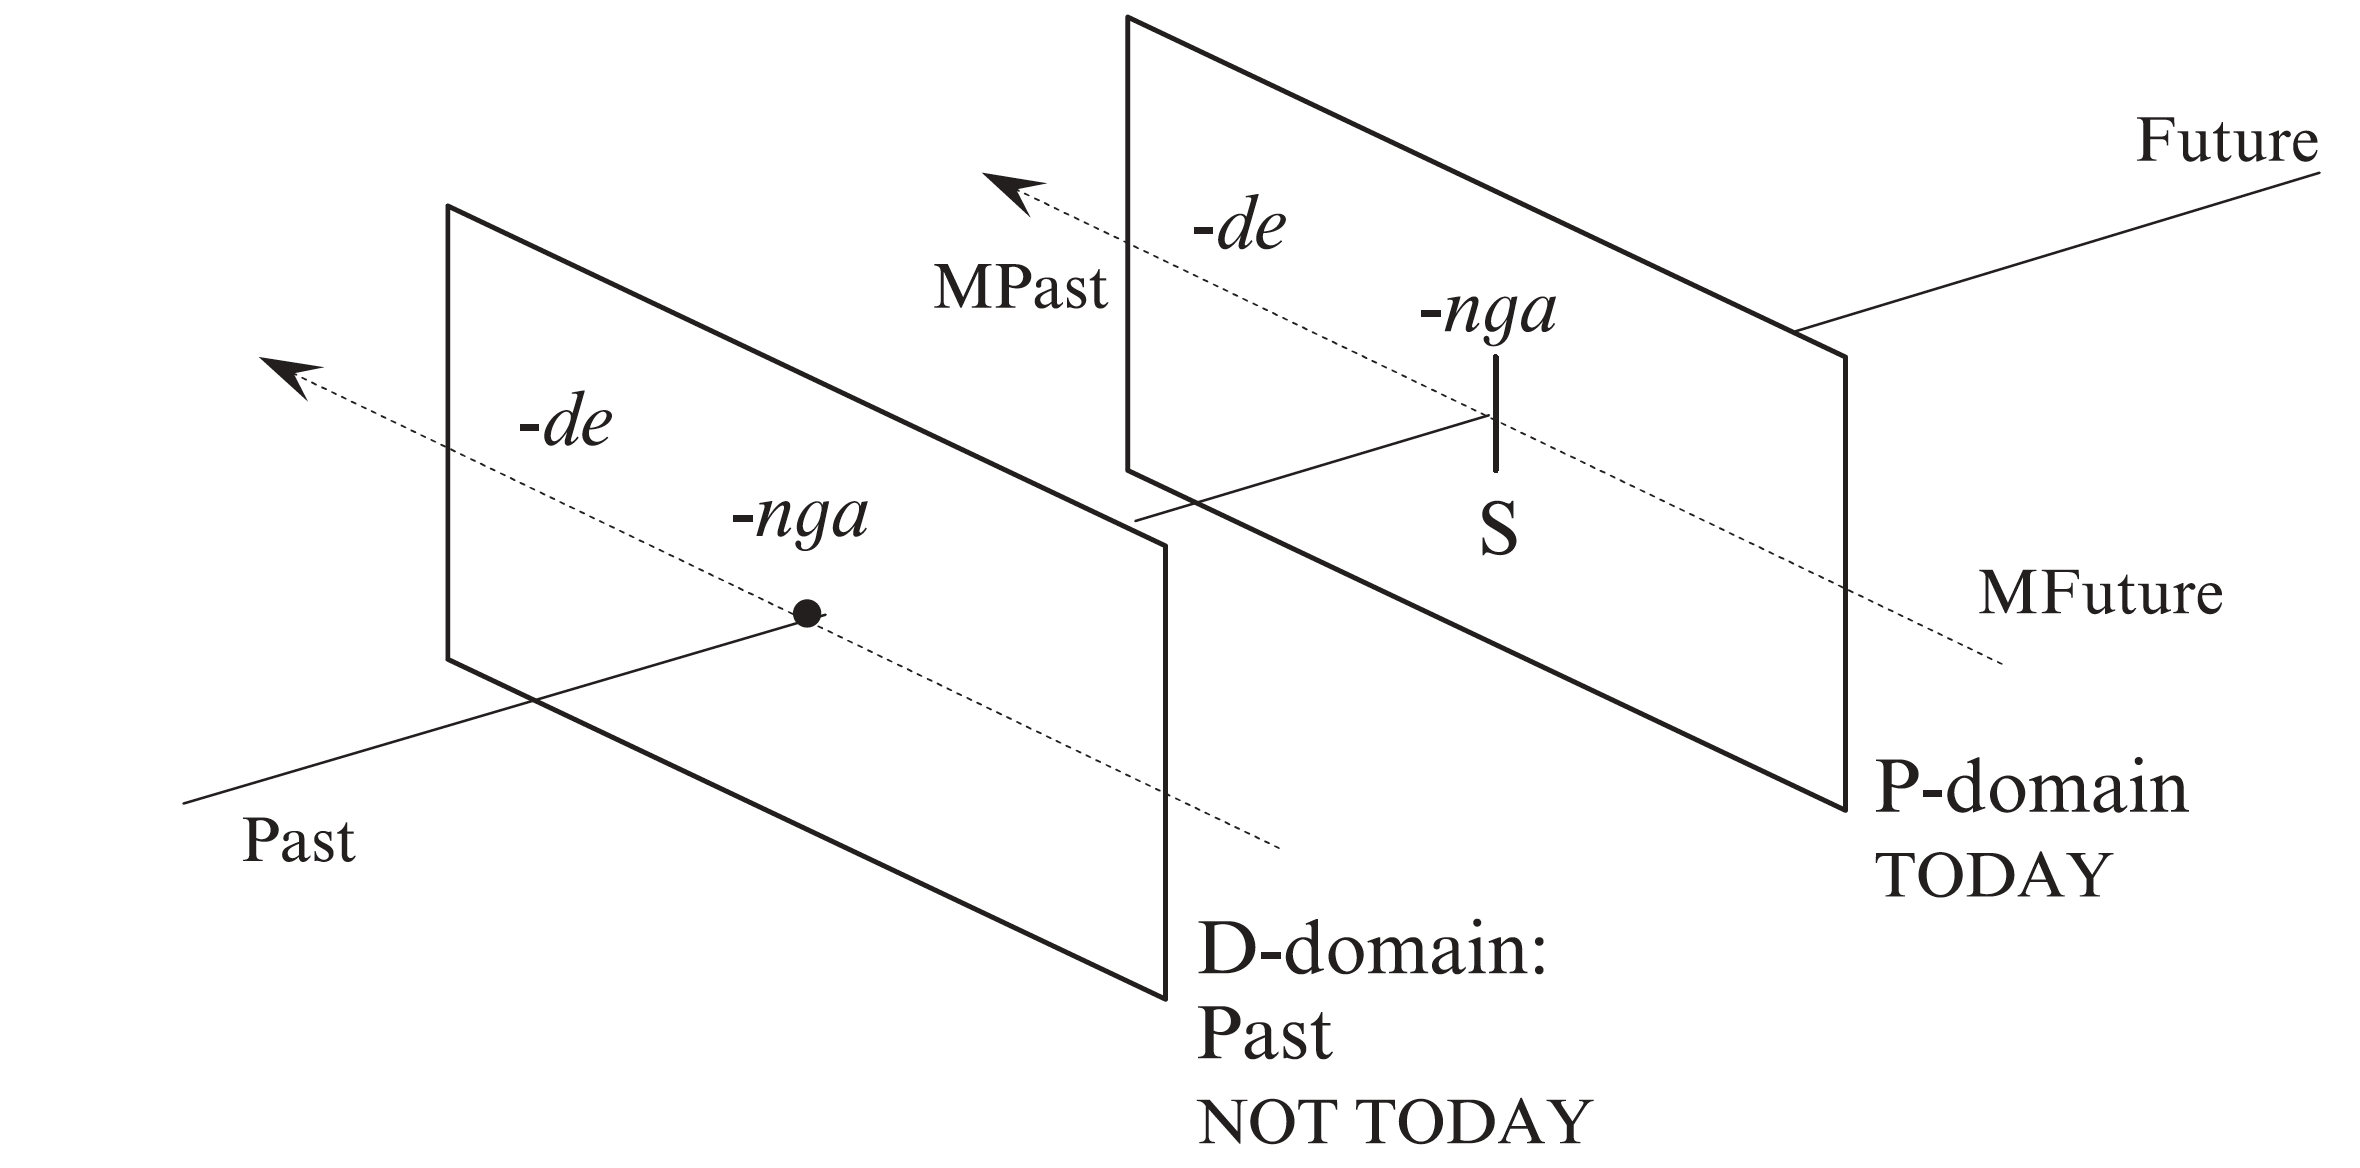
\includegraphics[width=0.9\linewidth]{botnecogdoms}
\end{figure}

\subsection{\textit{Énonciation}, diachrony \& functional unity}

For all the talk of reference frames and cognitive domains, how much closer are we to understanding the motivations for a the encoding of complex temporal remoteness systems of a grammaticalised cyclic tense system?

A number of linguists working on temporal/aspectual distinctions made in Indo\-European languages have drawn \citeauthor{Benveniste1966}'s distinction between ``narrative'' (\textit{récit\slash{}histoire}) and \textit{discours} modes (\textit{plans d'énonciation}).\footnote{Where ``\textit{\textbf{l'énonciation historique} [...] s'agit de la présentation des faits survenus à un certain moment de temps, sans aucune intervention du locuteur dans le récit}'' and \textit{\textbf{discours}} constitutes ``\textit{toute énonciation supposant un locuteur et un auditeur, et chez le premier l'intention d'influencer l'autre en quelque manière}''
	
	(``\textbf{Narrative} comprises the presentation of facts already having occurred at a given moment in time, without any intervention on the part of the speaker'' whereas \textbf{discourse} is understood as ``any utterance that presupposes a speaker and a hearer, where the former intends on influencing their interlocutor in some way.'')\trailingcitation{
	 \citetext{\citealp[238--42]{Benveniste1966}; translation and emphasis mine.}}} To take one example, \citeauthor{Duchet2016}'s \citeyearpar{Duchet2016} study of the usage domains of the Albanian [\gls{sqi}] \textit{\textsc{aorist}} and \textit{\textsc{perfect}},
 \footnote{That is, the synthetic `\textsc{aorist}' (\textit{e kryer e thjeshtë}) and the periphrastic `\textsc{perfect}' \textit{(e kryer)} form `\textsc{have}+past participle' respectively.} suggests the possible utility of this broad \textit{``énonciative''} dichotomy in understanding the distibution of these forms. While past-referring event descriptions in narrative contexts are the \textit{locus classicus} of the \textit{Aorist}, \citeauthor{Duchet2016} show that, in discourse contexts, using this form is also possible in a number of other apparent uses --- including the description of present-holding result states and ``immediate future'' accomplishments. The  \textit{Perfect}, traditionally encoding ``presently relevant result states'' (co-occurring frequently with TFAs that include speech time (`today/this week/this year') and in narratives to encode ``hot news'', also has a range of anterior-type uses: describing states (possibly) occurring prior to (\textsc{aorist-})marked past events.
 
Relatedly, in a survey of remoteness distinctions, \citet[116\textit{ff}]{Dahl1983} identifies a number of languages that appear to treat past differently in ``narrative contexts,'' going on to propose a number of cross-linguistic generalisations that seek to motivate a ``tendency to neutralize distance distinctions in narrative contexts.'' Drawing on a proposed distinction between narrative and discursive contexts, it is conceivable the two reference frames (\textsc{today\slash{}pre-today}) featuring into our analysis of \textsc{wd} temporal reference, in some sense, correspond respectively to \textbf{conversational} and \textbf{narrative} modes. 
 
 That is, in \textbf{conversational} contexts, described events are likely to bear a more immediate relation to the present. Here, a discourse is likely to be concerned with a distinction between {\color{blue}\textsc{past}} and {\color{forest}\textsc{nonpast}}. Conversely, in \textbf{narrative} contexts (accounts of exclusively past events), the distinction between events that held in a {\color{blue}\textsc{remote}}, inaccessible past versus those that held in a relatively \textsc{\color{forest}{recent}} one that more closely resembles the here-and now.\footnote{Compare \citeauthor{Waters1989}'s observation (in his description of Djinaŋ's \textsc{today/remote past}) that ``few stories are set in the time context of the same day as the speech event'' \citeyearpar[188]{Waters1989}.} This usage evokes the phenomenon of the ``narrative/historic present'' --- a commonly attested use cross-linguistically  \citetext{see \citealp{Carruthers2012} for an overview}.\footnote{Cited by \citet[312]{Carruthers2012}, \citeauthor{Facques2007} claims that the historic present ``permet de maintenir l’illusion d’une perspective simultanée du récit, déjà induite par l’emploi du present” (``
 	allows the	illusion to be maintained that the events and the narrative are simultaneous, an illusion already created by use of the present”) \citetext{\citeyear[250--1]{Facques2007}, Carruthers' translation.}} A similar usage of the \textsc{pres} (or \textsc{nonfuture}) is also pointed out by \citet{Stirling2012a}, who shows its extensive use in Kalaw Lagaw Ya [\gls{mwp}], where it functions as a past perfective in narrative contexts.\footnote{This type of usage is apparently widespread in Arnhem Land languages \citetext{\citealt[\textit{e.g.},][]{Bednall2019} for Anindilyakwa [\gls{aoi}]}}
 
On this account, the emergence of \textit{cyclic tense} of the type exhibited in the languages of Maningrida and the westernmost Yolŋu varieties (\textit{viz.} Djinaŋ, Djinba and \gls{wd}) can be explained in terms of a categoricalisation of these two ``reference frames'' that are closely associated with different modes of language use. This corresponds to a hypothetical analysis where: 
\begin{itemize}
	\item Language is used for conversation (pertaining to the eventualities that relate to the here-and-now) and for storytelling (pertaining to events completed prior to the here-and-now)
	\item The function of a \textsc{past}-tense is to signal the settledness and completeness of an event vis-à-vis utterance time. The function of \textsc{present} tenses indicates that the runtime of an event overlaps with utterance time.
	\item The \textsc{past}/\textsc{present} distinction gets reanalysed as \textsc{precontemporary}-{\sc contemporary}: that is \textsc{past/present} relative to a given reference frame (as determined by context (functions) of the utterance.)
\end{itemize}

\subsection{Aspect \& temporal interpreation}
As shown in \S~\ref{sec:djr-prs}, \textsc{wd} verb stems have a strictly dynamic (state change) semantics, a fact that seems to correspond with the recruitment of new strategies for encoding aspectual and modal information (primarily through preverbal auxiliaries and particles.)\footnote{Whereas an explicit aspectual (±\textsc{ipfv}) distinction is actually grammaticalised in the Djinaŋ verbal paradigm, a feature not shared by other Yolŋu languages} The development of this analytic TMA marking system in Dhuwal-Dhuwala is likely to be related to the emergence of a ``cyclic tense'' system where \gls{I} (the erstwhile `\gls{pres}') now obligatorily co-occurs with \textit{ga} `\gls{ipfv}' in order to encode present reference. Compare this fact to the incompatibility between present reference and achievement predicates, where a sentence of the type exemplified in (\nextx) is only available with either a historic present or immediate future reading \citep[an observation following][147]{Vendler1957}.


\pex\textit{Now they find the treasure/win the race/reach the summit}\xe
\pex\a\begingl\gla ŋarra *(ga) \textbf{ḻuka} mänha (dhiyaŋu~bala)\deftagex{wd-contemp}\deftaglabel{prog}//
\glb 1s \gls{ipfv}.\gls{I} drink.\gls{I} water now//
\glft`I'm drinking water (now).'\trailingcitation{[DB~20190405]}//\endgl
\a\begingl\gla ŋarra *(dhu) \textbf{ḻuka} mänha (dhiyaŋu~bala)\deftaglabel{fut}//
\glb 1s \gls{fut} drink.\gls{I} water now//
\glft`I'm going to drink water (now).'\trailingcitation{[DB~20190405]}//\endgl
\a\begingl\gla ŋarra \textbf{ḻuka} mänha (barpuru)//
\glb 1s \gls{ipfv}.\gls{I} drink.\gls{I} water//
\glft`I drank water yesterday.'\trailingcitation{[DB~20190405]}\deftaglabel{pst}//\endgl

\xe

This resembles the situation in \textsc{wd} (\getref{wd-contemp}), where \gls{I} necessarily co-occurs with \textit{ga} `\gls{ipfv}.\gls{I}' or \textit{dhu} `\gls{fut}' to encode present (progressive) or immediate future reference. In the absence of either of these markers, only the \textsc{recent (non-today) past} reading is felicitous.

The relationship between the emergence of cyclic tense in \gls{wd} and evidence for a wholesale restructuring of the language's aspectual system remain a subject for considerable further work and analysis.

\fancybreak

\noindent In view of the semantics for \gls{I} and \gls{III} above, this section has considered possible candidates for functional motivations for the notion of the ``reference frame'' and the ``recycling'' or ``temporal discontinuity'' of tense markers that characterise cyclic tense. On the basis of these considerations, (\nextx) formulates a hypothesis for the emergence of a cyclic tense system of the type described here.

\pex \textbf{\textsc{diachronic hypothesis.}\\Cyclicity as the grammaticalisation of text type}\\
The cyclic tense phenomena exhibited in \textsc{wd} and related languages are a result of the reanalysis of \textsc{present}- and \textsc{past}-tense markers' apparently divergent usage in conversational versus narrative contexts
\xe




 

\section{Conclusion}


This chapter has provided analyses for a number of phenomena related to the temporal interpretation of \textsc{wd} predicates. Of particular importance for developing an analysis of the \textsc{wd} paradigm and \gls{wd}'s tense system is the notion of \textsc{precontemporary instantiation}, a motivation for which was the primary focus of \S~\ref{sec:cyc}.

Drawing on descriptions from \citet{Glasgow1964} and subsequent treatments of the languages of western and central Arnhem Land \citep{Green1987,Green1995,Wilkinson1991,Eather2011,Waters1989}, we proposed a formal treatment of the notion of the ``reference frame'' --- effectively a \textsc{hodiernal/prehodiernal} dichotomy in the \textsc{nonfuture} (``\textsc{realis/actual}'') domain which corresponds to a superinterval of the reference time.

It was argued that the contribution of \gls{III} (the \textsc{precontemporary}) is to constrain reference time to a \textsc{non-final} subinterval of the contextually-supplied reference frame. Via blocking, instantiation of predicates inflected with \gls{I} are felicitous only within the complement of \gls{III}'s range within the realis domain. That is, \gls{I} --- an inflection compatible with present, past and future reference --- is an unmarked form, temporally neutral in its semantics \citetext{compare to treatments of the present, \textit{e.g.}, \citealp{Fleischman1990,Carruthers2012}.\footnote{Also \citeauthor{Dahl1983}'s generalisation that ``[i]t is almost always possible to use the least marked indicative verb form in a narrative past context'' (\citeyear[117]{Dahl1983}, \textit{apud} \citealt{Dahl1980} \textit{n.v}.)}}

 The following chapter extends the account to \gls{II} and \gls{IV} --- the irrealis categories.

%\begin{quote}\small Such meanings probably develop through the interaction of the meaning of the two grams. If a hodiernal past and an anterior (with current relevance) are both developing in the language they would both have a claim to describe situations having just occurred on the same day. If the anterior wins for situations that just occurred but the hodiernal continues to function for situations earlier in the same day, then the result is a discontinuous meaning for the non-hodiernal gram.\trailingcitation{\citep[104]{Bybee1994}}\end{quote}


%\pex
%
%\a \begingl\gla  ŋarra rur'yuna yurruna walu dha-barkthurruna//
%\glft`.'//\endgl
%
%

%
%\xe


\chapter{Modal interpretation \& \textsc{negative asymmetry}\\{\large\sc distinguishing $\boldmath{ \langle \gls{I},\gls{III}\rangle}$ from $\boldmath{ \langle \gls{II},\gls{IV}\rangle}$}}\label{sec:yol-mood}

The basic distributional facts for \gls{II} and \gls{IV} were described in \S~\ref{djr-infl}. As shown there, verb stems receive \gls{II}-marking in future-oriented predications (including imperatives), whereas \gls{IV}-marking is associated most clearly with counterfactual predications and other modal claims with past temporal reference. On the basis of these data, these two inflectional categories appear to be associated with \textit{non-realised} events; and it is this property that distinguishes them from the \gls{I}- and \gls{III}-marked verbs described in the previous chapter (ch.~\ref{sec:djr-temp}).

In this chapter, we interrogate the nature of this apparent ``reality status'' distinction drawn in \gls{wd} (as it is in other Yolŋu Matha varieties) and the expression of mood, modality and modal operators in \gls{wd} more broadly. The distinction between $\langle \gls{I},\gls{III}\rangle$ and $\langle \gls{II},\gls{IV}\rangle$ is ultimately to be understood as one of \textsc{verbal mood}. One phenomenon of particular interest is that of an apparent kinship between negative operators (sentential negators) and modal operators as they are realised in \gls{wd}. It is this kinship that looks to undergird \textit{asymmetric negation} in \textsc{wd} with respect to the marking of reality status; a description of this phenomenon is the goal of \S~\ref{sec:negs}.

\section{Sentential negation and paradigm neutralisation}\label{sec:negs}

As shown in our discussion of the Negative Existential Cycle in Yolŋu Matha (\S~\ref{NEC-yolŋu}, see \textit{p.}~\pageref{sec:nec-djr}), Djambarrpuyŋu has two particles---\textit{yaka} and \textit{bäyŋu}---which both realise standard negation (\textit{i.e.}, that operator whose effect is to reverse the truth value of a given proposition.) The primary distributional distinction between these is that only \textit{yaka} is used to generate negative imperatives (prohibitives) whereas only \textit{bäyŋu} is found in negative existential/quantificational contexts (\getref{bayŋu-negq}--\getref{yaka}). Of interest for current purposes however, is the fact that both of these sentential negators can be shown to directly interact with verbal inflection.


Descriptively, as shown in the data in (\getref{neg-pres}--\getref{neg-pst}), negation appears to trigger a ``switch'' from the `realis-aligned inflections' (\gls{I}~and~\gls{III}) to their `irrealis counterparts' (respectively \gls{II}~and~\gls{IV}). As shown, these latter categories otherwise turn up predominantly in \textit{hypothetical} or \textit{counterfactual} contexts. As we will see, this points to an analysis where the Western Dhuwal(a) inflectional system encodes a \textit{reality status}-based distinction that is neutralised in negated sentences \citep[see also discussion in][356]{Wilkinson1991}. This effect --- which we term a ``negative asymmetry'' \citep[specifically \textsc{\texttt{a/nonreal}}, following][]{Miestamo2005} --- was introduced above (\S~\ref{sec:asymneg}, compare the Gurr-goni \gls{gge} data in \getref{sn-gvg})  and is summarised below in Table \ref{tab:negneut}. Here, we develop a theory of the negative asymmetry as an epiphenomenon of a kinship between \textsc{negative} and (other) \textsc{irrealis} operators.

\begin{table}[h]\centering
	\begin{tabular}{ccc}
		&\multicolumn{2}{c}{\textsc{\textbf{polarity}}} \\
		& \textsc{--neg} & \textsc{+neg}\\\midrule
		&	\gls{I} & \multirow{2}{*}{\gls{II}}\\
		& \gls{II} \\\midrule
		&	\gls{III} & \multirow{2}{*}{\gls{IV}}\\
		& \gls{IV} \\\bottomrule
	\end{tabular}
	\caption{Neutralisation of \gls{I} and \gls{III} inflections under negation.}\label{tab:negneut}
\end{table}


The following examples in (\getref{neg-pres}) show how sentences that receive \gls{I}-marking in positive sentences --- encoding temporal reference to the present or recent past (Ch.~\ref{sec:djr-temp}) --- instead receive \gls{II}-marking under the scope of negation. Each example contains a predication about the present or about the recent past (normally the domain of \gls{I}, as described in the previous chapter.) In thje presence of a negative operator, however, the verb receives \gls{II}-marking. 

(\getref{neg-pres}a-b), for example, presents a near-minimal pair, where the inflection received by a predicate with present reference ``switches'' from \gls{I} to \gls{II} under negation.

\pex\textbf{Exponence of present and recent past reference as \gls{II} under negation}
\deftagex{neg-pres}


\a\begingl%\glpreamble Present-tensed sentence with \gls{I}//
\gla Nhaltja-\textbf{n} \textbf{ga} limurru-ŋgu-ny rom waŋ-\textbf{a}?//
\glb do.how-\gls{I} \gls{ipfv}.\gls{I} 1p.\gls{incl}-\gls{dat}-\gls{prom} law say-\gls{I}//
\glft`What does our law say?'\trailingcitation{\citepalias[~Luk~14.3]{DB}}//\endgl

\a\begingl%\glpreamble Negated present-tense sentence receives \gls{II} marking//
\gla \textbf{yaka} \textbf{gi} \textbf{biyak} rom waŋ-\textbf{i}//
\glb \textbf{\gls{neg}} \gls{ipfv}.\gls{II} do.thusly.\gls{II} law say-\gls{II}//
\glft`That's not how the law is/what the law says.'\trailingcitation{\citep[357]{Wilkinson1991}}//\endgl 




\a\begingl%\glpreamble  Negated present-tense sentence receives \gls{II} marking\\\textsc{context.} Speaker is trying to read from a computer screen.//
\gla \textbf{bäyŋu} ŋarra \textbf{gi} nhä-\textbf{ŋu}//
\glb \textbf{\gls{negq}} 1s \gls{ipfv}.\gls{II} see-\gls{II}//
\glft`I can't see (it).'\\
%\textsc{comment.} \textit{nhäŋu} (`see.\gls{II}') could also mean yesterday in past.
\textsc{\textbf{comment.}} `I didn't see (it) (yesterday)' is also an available reading.\trailingcitation{[AW 2018030]}//\endgl



\a\begingl\gla Ŋarra \textbf{gi} bäyŋu maḻŋ'mara-\textbf{ŋu} waṯu (ŋarraku). + Bili ŋayi \textbf{ga} nhin-\textbf{a} wäŋaŋura//
\glb 1s \textsc{ipfv}.II \gls{neg} appear.\gls{caus}-\gls{II} dog 1s.\gls{dat} \gls{cplv} 3s \gls{ipfv}.\gls{I} sit.\gls{I} house.\gls{loc}//
\glft`I can't find my dog. It lives in the house.'\trailingcitation{[DhG~20190417]}//\endgl



\a\begingl\gla Ŋarra ga djäl-thi-\textbf{rri} giritjirrinyara-wu, + yurru ŋarra bäyŋu-nha \textbf{girritji}//
\glb 1s \gls{ipfv}.\gls{I} want-\gls{vblzr}-\gls{I} dance.\gls{nmlzr}-\gls{dat} but 1s \gls{neg}-\gls{seq} dance-\gls{II}//
\glft`I was wanting to dance (at the \textit{buŋguḻ} yesterday) but I didn't dance (because I'd hurt my leg yesterday.)'\trailingcitation{[DhG~20190417]}//\endgl
%\a\begingl\glpreamble\textsc{context.} A recent hunting trip, narrated in \gls{I} for corresponding positive descriptions.//
%\gla ga \textbf{yaka} ŋayi ŋunhi dharyu-\textbf{rr} \textbf{biyak} djin'tjiŋdhu-\textbf{rr}//
%\glb and \textbf{\gls{neg}} 3s \gls{texd} rain-\gls{II} do.thusly.\gls{II} rain~lightly.\gls{II}//
%\glft`...and it did not rain lightly'\trailingcitation{\citep[357]{Wilkinson1991}}/endgl
\xe


Similarly, in contexts where the temporal reference of the event description predicts that the verb will receive \gls{III}-inflection --- following our description from Ch. \ref{sec:djr-temp}, when referring to the same-day (\textsc{hodiernal}) or the remote past --- when co-occurring with a negative particle (\textit{yaka/bäyŋu}), the verb instead receives \gls{IV}-inflection. This is shown by the data in (\getref{neg-pst}).

 Again, (\getref{neg-pst}a-b) represents a minimal pair where negative marking triggers a ``switch'' from \gls{III} to \gls{IV} inflection. (c) shows the negation of an immediate past event licensing \gls{IV} inflection, (d) shows how a negated, \gls{IV}-inflected predicate can be embedded under a propositional attitude predicate to encode a false belief, and (e) an example of a negated description of the remote past receives \gls{IV} inflection.

\pex \textbf{Exponence of \textsc{today past} and \textsc{remote past} reference as \gls{IV} under negation}\deftagex{neg-pst}
%\a\deftaglabel{munha}\begingl\gla bäyŋu ŋarra gäthur ŋorra-\textbf{nha} manymak-ku-\textbf{nha} munhawu//
%\glb \gls{negq} 1s today lie-\gls{IV} good-\gls{tr}-\gls{IV} nighttime//
%\glft`I didn't sleep well last night'\trailingcitation{\citep[357]{Wilkinson1991}}//\endgl

%\mcom{Though the second clause in (b) also has ŋuli so maybe this is not quite so nice an ex. as originally thought}\a\begingl\gla ŋäthil-nydja ŋarra ga-n dhuwal, ga miltjiri marrtji-n \ bäyŋu ŋarra ŋuli ga-\textbf{nha} nhä-\textbf{nha}//
%\glb earlier-\gls{prom} 1s \gls{ipfv}-\gls{III} \gls{prox} and blind go-\gls{III} \textbackslash \gls{negq} 1s \gls{hab} \gls{ipfv} see-\gls{IV}//
%\glft`I was blind before; I was unable to see'\trailingcitation{\citep[358]{Wilkinson1991}}//\endgl


\a\begingl\gla gathur munhagumirr ŋarra nhä-\textbf{ŋal} warrakan//
\glb today morning 1s see-\gls{III} bird//
\glft`I saw a bird this morning'\trailingcitation{[FW 20180802]}//\endgl


\a\begingl\gla gathur munhagumirr \textbf{bäyŋu} ŋarra nhä-\textbf{nha} warrakan//
\glb today morning \textbf{\gls{negq}} 1s see-\gls{IV} bird//
\glft`I didn't see a bird this morning'\trailingcitation{[FW 20180802]}//\endgl

\a\begingl\glpreamble \textsc{\textbf{context}.} Speaker has dropped a coin.//
\gla Way! \textbf{Bäyŋu} ŋarra nhä-\textbf{nha}?//
\glb Hey! \textbf{\gls{negq}} 1s see-\gls{IV}//
\glft`Ah! Did you see (it)?'\trailingcitation{[AW 20180830]}//\endgl


\a\begingl\glpreamble\textbf{\textsc{context.}} I'm at work explaining to my coworker why my \textit{galay} is angry at me.//
\gla Ŋarraku miyalk maḏakarritj-thi-\textbf{na} bili ŋayi ga \textbf{guyaŋa} ŋarra ga-\textbf{nha} bäyŋu djäma//
\glb 1s.\gls{dat} wife anger-\gls{inch}-\gls{III} \gls{cplv} 3s \gls{ipfv}.\gls{I} think.\gls{I}\footnotemark{} 1s \gls{ipfv}-\gls{IV} \gls{neg} work//
\glft`My wife got angry because she thought I wasn't working today.'\trailingcitation{[DhG~20190417]}//\endgl

\a\begingl\glpreamble \textbf{\textsc{context.}} The speaker grew up in the desert.//
\gla \textbf{bäyŋu} ŋarra ŋuli ga-\textbf{nha} nhä-\textbf{nha} (waltjaṉ) ŋunhi ŋarra yothu yän//
\glb \textbf{\gls{neg}} 1s 	\gls{hab} \gls{ipfv}.\gls{IV} see.\gls{IV} rain \gls{texd} 1s child just//
\glft`When I was young, I hadn't seen [rain]/never saw [rain].'\trailingcitation{[AW~20190501]}//\endgl\xe


%\mcom{It's not clear how I can easily get a the status of this alternation via elicitation (esp. if its intraspeaker..?) or whether I should just abstract away from it. My informants so far seem to have consistently respected this alternation.}
%todo comments about variation across Dhuwal/a
%	Generally, there seems to be a perception (Melanie Wilkinson \textit{pers. comm.}, independently supported by consultant AW [20180830]) that the maintenance of \gls{I} and \gls{III} (the `\textsc{realis}-aligned' inflections) under negation is a characteristic of \textit{Miwatj} varieties of Dhuwal-Dhuwala (\textit{i.e.}, those spoken in towards the East.)
%	
%	\mcom{There's a great comment from my consultant in her translation of a negative sentence. When asked why \textbf{\textit{gi+}II} was used instead of \textbf{\textit{ga+}I} she claims `not happening yet' (20180802-8min)}\citet[356]{Wilkinson1991} notes that ``[she has] not been able to determine a functional basis for this alternation.'' Nevertheless, in his typological survey of standard negation, \citet[558]{Miestamo2005} identifies a cross-linguistically attested mood-based asymmetry where negative marking triggers the appearance of the irrealis or other ``nonrealised''-type modal markings. This phenomenon seems to be particularly well-represented in the languages of the Top End, functional explanations generally emphasising the fact that negated predicates `[belong] to the realm of the non-realized', a domain associated with irrealis marking (\citealt[225]{Miestamo2005}, cf. \citealt[195]{McLellan1992}, \citealp[see also][]{Phillips2019}). These ideas are explored in further detail in Chapter \ref{anY} below.
%	
%	\citet{Wilkinson1991} also suggests that there is insufficient cross-linguistic data to assess a the diachrony (and potential areal diffusion) of this asymmetry (356), although provides a concise review of other authors' observations of Yolŋu varieties (359-60). Data about the interactions between polarity and verbal inflection are provided in the following sections and the question of the development of these asymmetries is treated in Chapter \ref{diaY} below.

The data in (\getref{neg-pres}--\getref{neg-pst}) evince a species of \textsc{negative asymmetry} that is manifested in \gls{wd}. That is, from the four inflections which are availble for encoding temporal and modal information in \gls{wd}, only two (\textit{viz.} \gls{II} and \gls{IV}) are felicitous in sentences that are negated by \textit{yaka} or \textit{bäyŋu}. Figure \ref{NegSchem} schematises the relationship between temporal reference and inflection selection in \textbf{negative clauses} (\textit{cf.} Fig.~\ref{TempSchem}, \textit{p.}~\pageref{TempSchem}.)


\begin{figure}[h]\centering\caption{Apparent interactions between temporal relations and reality status in Djambarrpuyŋu: cyclicty and metricality under negation.}\label{NegSchem}
	\begin{tikzpicture}[scale=1.2]
		% draw horizontal line   
		\draw[<->, line width=.5mm] (0,0) -- (12,0);
		
		%draw rex
		\shade[left color=violet!15!white, right color=orange!15!white] (0,0.02) rectangle (4.8,1.5);
		%	\fill[green!10!white] (2.5,0.02) rectangle (4.8,1.5);
		\fill[violet!10!white] (4.8,0.02) rectangle (6.8,1.5);
		\shade[left color=orange!10!white, right color=green!10!white] (6.8,0.02) rectangle (9.5,1.5);
		\fill[orange!10!white] (9.5,0.02) rectangle (12,1.5);
		
		% draw nodes
		\draw (1.25,0) node[below=3pt] {\textbf{}} node[above=15pt] {\textsc{\gls{IV}}};
		\draw (3.675,0) node[below=3pt] {\textbf{}} node[above=15pt] {\gls{II}};
		\draw (5,0)   node[circle,fill,label=below:$\lfloor{\sl today}$] {} node[below=3pt] {\textbf{}} node[above=3pt] {};
		\draw (7,0) node[diamond,shade,inner color=ochre,outer color=black,label=below:$\boldsymbol{t*}$] {} node[below=3pt] {\textbf{}} node[above=3pt] {\textsc{}};
		\draw (5.8,0) node[below=3pt] {\textbf{}} node[above=15pt] {\textsc{\gls{IV}}};	
		\draw (7.5,0) node[below=3pt] {\textbf{}} node[above=15pt] {\textsc{\gls{II}}};
		\draw (9,0) node[below=3pt] {\textbf{}} node[above=15pt] {\textsc{\gls{I}}};	
		\draw (10.75,0) node[below=3pt] {\textbf{}} node[above=15pt] {\textsc{\gls{II}}};	
		\draw (9.5,0)   node[circle,fill,label=below:${\sl today}\big)$] {} node[below=3pt] {\textbf{}} node[above=3pt] {};
		
		%		%braces
		%		\phantom{	\draw [decorate,decoration={brace,amplitude=4pt},xshift=-0pt,yshift=35pt]
		%			(0.5,0.5) -- (4.5,0.5) node [black,midway,yshift=0.35cm] 
		%			{\footnotesize metricality};
		%
		%			\draw [decorate,decoration={brace,amplitude=4pt},xshift=-0pt,yshift=40pt]
		%			(3.5,0.5) -- (9,0.5) node [black,midway,yshift=0.35cm] 
		%			{\footnotesize cyclicity};}
		
	\end{tikzpicture}
\end{figure}

Further complicating things, while \gls{III} is categorically ruled out in negative sentences, \gls{I} ``survives'' when (and \underline{only when}) the predicate refers to the \textsc{same-day future.} That is, the \gls{I}/\gls{II} distinction is \textit{not} neutralised in negative sentences with reference to events happening later on the day of utterance (whereas the distinction \textit{is} neutralised in all \textsc{nonfuture} contexts.) Examples are provided in (\getref{futneg}-\getref{prsneg}).


\pex \textbf{Future marking is unaffected by polarity/the presence or absence of sentential negation}	\deftagex{futneg}
\a\begingl\glpreamble \gls{I} with \textsc{same-day future} reference ``survives'' negation//
\gla ŋarra (yaka) ŋunha \textbf{dhu} ḻuk-\textbf{a} dhiyaŋ~bala//
\glb 1s (\gls{neg}) \gls{fut} \gls{dist} eat-\gls{I} now//
\glft`I will (not) eat them [\textit{ḻatjin}] right now.'\trailingcitation{[AW~20190422]}//\endgl

\a\begingl\glpreamble \textsc{post-hodiernal} referring predicates receive \gls{II}-inflection//
\gla (bäyŋu) ŋarra \textbf{dhu} buḻ'yu-\textbf{rr} barpuru//
\glb \gls{neg} 1s \gls{fut} play-\gls{II} tomorrow//
\glft`I will (not) play [football] tomorrow.'\trailingcitation{[AW~20190429]}//\endgl
\xe

\pex \textbf{A minimal pair: \gls{I} changes to \gls{II} in present-referring negative sentences}\deftagex{prsneg}
\a\begingl\glpreamble Negative present predication with \gls{II}//
\gla (dhiyaŋ~bala) \textbf{bäyŋu} ŋarra \textbf{gi} nhä-\textbf{ŋu} mukulnha//
\glb now \textbf{\gls{neg}} 1s \gls{ipfv}.\gls{II} see-\gls{II} aunt.\gls{acc}//
\glft`I don't/can't see my aunt (right now).'\trailingcitation{[AW~20190501]}//\endgl
\a\begingl\glpreamble Positive present predication with \gls{I}//
\gla (dhiyaŋ~bala)  ŋarra \textbf{ga} nhä-\textbf{ma} mukulnha//
\glb now 1s \gls{ipfv}.\gls{I} see-\gls{I} aunt.\gls{acc}//
\glft`I'm watching my aunt (right now).'//
\endgl\xe


\section{The meaning of the modal particles}
\label{sec:modals}
%todo label `anY' has been de-defined
%\section{The realm of the nonrealized}\label{anY}
In \S~\ref{djr-infl}, we saw that predicates which receive \gls{II}- and \gls{IV}-inflection co-occur with some operator that encodes some flavour of irrealis-associated meaning --- suggesting what \citet[145]{Palmer2001} labels a ``joint marking system'' (\textit{i.e.}, that reality is multiply indicated, in this case by suffixation in addition to a preverbal particle.) 

For \gls{II}, these are predominantly represented by \textit{dhu} `\gls{fut}' and \textit{balaŋ(u)} `\gls{irr}' in addition to clauses with imperative syntax. \gls{IV} tends to co-occur with \textit{balaŋ} `\gls{irr}' in addition to \textit{ŋuli} `\gls{hab}'.\footnote{I adopt the (metalinguistic) labels \gls{fut} for \textit{dhu} \citep[following][]{Wilkinson1991} and \gls{mod} for \textit{balaŋ(u)}. As we will see, these descriptions aren't necessarily completely semantically adequate, but will be sufficient for current purposes. \citet{Wilkinson1991} glosses \textit{ŋuli} as `\gls{hab}' or `\gls{hyp}' depending on its apparent function in the clause (as a marker of \textsc{habituality} or of a conditional antecedent (``\textsc{hypotheticality}'').)\label{irr-glossing}} Importantly, and as we will see, these expressions all appear to lexicalise strictly \textbf{root} (circumstantial\slash{}non-epistemic) modalities \citep[\textit{contra claims in}][123]{VanderWal1992}.

This section seeks to model the irrealis domain using the ``branching time framework'' introduced in \S~\ref{LitRev} in order to propose a semantics for \gls{wd} modal particles. This will permit for forming a set of generalisations over the distribution of \gls{II} and \gls{IV}.



	%\subsection{The branching time framework}\label{sec:wd-BT-fwk}
	%
	%Authors working in intensional semantics have, in recent work, deployed a ``branching time'' framework in order to model relationships between temporal and modal reference (an overview provided in Chapter \ref{IntroCh} and implemented in the semantic treatment of \textit{bambai} in Chapter \ref{bambai.semx}). Here, I spell out a number of basic assumptions that will ultimately assist in formalising temporal and modal expressions in WD. One of the primary payoffs of the branching time is the formalisation of Prior's observations about the asymmetries of the past and the future \citep[see also][]{Copeland2020,Dowty1977,Thomason1970,Thomason1984}. The version I adopt here follows closely from recent work on the realis-irrealis distinction \citep{VonPrince2019,Krifka2016} and other insights about temporal and modal interaction (\citealp[e.g.][]{Condoravdi2002,Ippolito2013}, a.o.)
	%
	%
	%A branching-time frame $ \mathfrak U=\langle \mathcal I,\prec\rangle $ assumes a partially ordered set of indices $ \mathcal I $ --- in effect world-time pairs $ \langle w,t\rangle  $. A branch (similar to ``history'' for other authors \citep{Thomason1970,Dowty1977}) $ b\ni i $ through any $ i\in\mathcal I $ is a linearly ordered subset of $ \mathcal I $ --- that is, where $ i=\langle w,t\rangle $,\\ $ b\ni i=\{\big\langle\langle w,t\rangle,\langle w,t'\rangle,\langle w,t''\rangle,\hdots,\langle w,t_n\rangle\big\rangle\}$. A branch, then, effectively models the possible development of a given world through time.\footnote{Note that these frameworks normally take indices to represent world-time pairs. I assume that this model can be extended relatively straightforwardly to capture interval semantic notions (\citealp[e.g.][]{Landman1991,Dowty1982,Bennett} a.o.).}
	%\begin{figure}[h]
	%	\caption{A branching times frame following von Prince \citeyearpar[e.g.,][591]{VonPrince2019}. Vertically aligned indices are taken to index the same time.}\centering
	%	\begin{tikzpicture}
	%		[scale=1.5,level distance=9mm,
	%		every node/.style={fill=black,circle,inner sep=1.5pt},
	%		level 1/.style={sibling distance=10mm},
	%		level 2/.style={sibling distance=8mm},
	%		level 3/.style={sibling distance=4mm},
	%		level 4/.style={sibling distance=2mm},
	%		edge from parent/.style={draw}]
	%		\node {} [grow=right]
	%		child {node {} edge from parent[densely dotted]
	%			child {node {}
	%				child {node {}
	%					child {node {}}
	%					child {node {}}}
	%				child {node {}
	%					child {node {}}
	%					child {node {}}}}
	%			child {node {}
	%				child {node {}
	%					child {node {}}
	%					child {node {}}}
	%				child {node {}
	%					child {node {}}
	%					child {node {}}}}}
	%		child[missing]
	%		child {node {}
	%			child {node {} edge from parent[densely dotted]
	%				child {node {}
	%					child {node {}}
	%					child {node {}}}
	%				child {node {}
	%					child {node {}}
	%					child {node {}}}}
	%			child {node {} edge from parent[densely dotted]
	%				child {node {}
	%					child {node {}}
	%					child {node {}}}
	%				child {node {}
	%					child {node {}}
	%					child {node {}}}}
	%			child {node [style={fill=red},label=above:$ \boldsymbol{i*} $] {}
	%				child {node {} edge from parent[densely dashed]
	%					child {node {}}
	%					child {node {}}}
	%				child {node {} edge from parent[densely dashed]
	%					child {node {}}
	%					child {node {}}}}};
	%\end{tikzpicture}\end{figure}
	%
	%
	%
	%
	%
	%
	%
	%\Citet{VonPrince2017a,VonPrince2019} establishes a formal trichotomy between the \textsc{actual, potential} and \textsc{counterfactual} domains by appealing to this framework. This is reproduced in (\nextx).
	%
	%\pex Given a contextually defined \textsc{actual present} $( i*=\langle w*,t*\rangle )$, $ \mathcal I $ can be partitioned into three subdomains:
	%\a The \textsc{actual} (past/present) = $ \{i\mid i\preceq i*\} $\\
	%Compare this notion to the equivalent one of \textit{metaphysical alternatives to $ w $ at $ t $} introduced in Ch. \ref{bambai}: $ \{w'\mid w\approx_t w\} $.
	%\a The \textsc{potential} (future) = $ \{i\mid i\succ i*\} $
	%\a The \textsc{counterfactual} = $ \{i\mid i \text{ is unordered w/r/t } i* \} $\deftagex{trichot}\deftagpage{vP-bt}
	%\xe





\subsection{\textit{dhu}: irreality and the \textsc{future}}

Shown above (predominantly in \S~\ref{desc-ii}),  \textit{dhu} `\gls{fut}' occurs in sentences with future temporal reference -- with either \gls{I} or \gls{II} marking, depending on whether the reference time of the proposition is the same as the day of speech or beyond. This is shown again by the data in \getref{dhu-fut}.

Relatedly, the data in (\getref{dhu-nec}) show that \textit{dhu} appears to also be compatible with other circumstantial modalities; for example, with (\getref{dhu-nec.d}) deontic, (\getref{dhu-nec.b}) bouletic and (\getref{dhu-nec.t}) teleological readings. In all these contexts, we can model \textit{dhu} as universally quantifying over a (subset of) a circumstantial modal base.

\pex \textbf{\textit{dhu} `\gls{fut}' encoding future tense with \gls{I}- and \gls{II}-inflections}
\a\begingl\gla barpuru goḏarr ŋarra \textbf{dhu} nhä-\textbf{ŋu}//
\glb funeral tomorrow 1s \gls{fut} see-\gls{II}//
\glft`I'll watch the funeral tomorrow.'\trailingcitation{}\deftagex{dhu-fut}//
\endgl
\a\begingl\gla mukul \textbf{dhu} \textbf{gi} nhin-\textbf{i} raŋi-ŋur goḏarr//
\glb aunt \textbf{\gls{fut}} \gls{ipfv}.\gls{II} sit-\gls{II} beach-\gls{loc} tomorrow//
\glft`Aunty will be sitting on the beach tomorrow.'\trailingcitation{[AW~20190409]}//\endgl
\a\begingl\gla limurru \textbf{dhu} ḻuk-\textbf{a} maypal yalala milmitjpa//
\glb 1d.\textsc{excl} \textsc{fut} consume-\gls{I} shellfish later evening//
\glft `We're having shellfish this evening.'\trailingcitation{[DhG~20190417]}//
\endgl
\xe
\pex \textbf{\textit{dhu} `\gls{fut}' and other flavours of modal necessity}\deftagex{dhu-nec}
\a\begingl\gla Way! Nhe \textbf{dhu} gurruk-\textbf{ama} djoŋgu'!//
\glb Hey! 2s \gls{fut} carry-\gls{I} hat//
\glft`Hey! You must wear a helmet!'\trailingcitation{[DhG~20190405]}\deftaglabel{d}//\endgl
\a\begingl\gla djamarrkuḻi \textbf{dhu} yaka wurraŋatjarra'\textbf{y-irr}\deftaglabel{b}//
\glb children \gls{fut} \gls{neg} cruel.\gls{inch}-\gls{I}//
\glft`The children mustn't be disobedient.'\trailingcitation{[AW~20190429]}//\endgl
\a\begingl\gla ŋarra \textbf{dhu} plane-dhu marrtji, bili mutika-miriw\deftaglabel{t}//
\glb 1s \gls{fut} plane-\gls{erg} go-\gls{I}|\gls{II} \gls{cplv} car-\gls{priv}//
\glft`I'll have to go by plane because I don't have a car.'\trailingcitation{[AW~20190429]}//\endgl
\xe

\noindent Suggested in \S~\ref{desc-ii}, \textit{dhu} appears exclusively in \textit{future-oriented} predications, apparently \textit{with present perspective} (that is, in predications about the future as calculated at speechtime, \citealp[see][]{Condoravdi2002}.) The relation between temporal reference and inflection in \textit{dhu-}marked sentences is schematised in figure \ref{FutSchem}.

\begin{figure}[h]\centering\caption{(In)compatibility of modal particle \textit{dhu} `\gls{fut}' with temporal reference \& inflectional category.}\label{FutSchem}
	\begin{tikzpicture}[scale=.9]
		% draw horizontal line   
		\draw[<->, line width=.5mm] (0,0) -- (12,0);
		
		%draw rex
		\fill[gray!10!white] (0,0.02) rectangle (4.8,1.5);
		%	\fill[green!10!white] (2.5,0.02) rectangle (4.8,1.5);
		\fill[gray!10!white] (4.8,0.02) rectangle (6.8,1.5);
		\fill[green!10!white] (6.8,0.02) rectangle (9.5,1.5);
		\fill[orange!10!white] (9.5,0.02) rectangle (12,1.5);
		
		% draw nodes
		\draw (1.25,0) node[below=3pt] {\textbf{}} node[above=10pt] {\textsc{\textbf{*}}};
		\draw (3.675,0) node[below=3pt] {\textbf{}} node[above=10pt] {\textbf{*}};
		\draw (5,0)   node[circle,fill,label=below:$\lfloor{\sl today}$] {} node[below=3pt] {\textbf{}} node[above=3pt] {};
		\draw (7,0) node[diamond,shade,inner color=ochre,outer color=black,label=below:$\boldsymbol{t*}$] {} node[below=3pt] {\textbf{}} node[above=3pt] {\textsc{}};
		\draw (5.8,0) node[below=3pt] {\textbf{}} node[above=10pt] {\textsc{\textbf{*}}};	
%		\draw (7.5,0) node[below=3pt] {\textbf{}} node[above=10pt] {\textsc{\gls{II}}};
		\draw (8.25,0) node[below=3pt] {\textbf{}} node[above=10pt] {\textsc{\gls{I}}};	
		\draw (10.75,0) node[below=3pt] {\textbf{}} node[above=10pt] {\textsc{\gls{II}}};	
		\draw (9.5,0)   node[circle,fill,label=below:${\sl today}\big)$] {} node[below=3pt] {\textbf{}} node[above=3pt] {};
		
		%		%braces
		%		\phantom{	\draw [decorate,decoration={brace,amplitude=4pt},xshift=-0pt,yshift=35pt]
		%			(0.5,0.5) -- (4.5,0.5) node [black,midway,yshift=0.35cm] 
		%			{\footnotesize metricality};
		%
		%			\draw [decorate,decoration={brace,amplitude=4pt},xshift=-0pt,yshift=40pt]
		%			(3.5,0.5) -- (9,0.5) node [black,midway,yshift=0.35cm] 
		%			{\footnotesize cyclicity};}
		
	\end{tikzpicture}
\end{figure}


\noindent On the basis of this range of usage, we have reason to treat \textit{dhu} as a modal expression. Here we adopt the quantificational (pragmatic domain restriction) approach to modal semantics introduced in \S~\ref{sec:kratzer} and adapt an analysis in the style of \citeauthor{Condoravdi2003}'s (\citeyear{Condoravdi2002,Condoravdi2003} a.o.) unified treatment of \textit{will} on its `future auxiliary' and modal uses .


The different ``flavours'' of \textit{dhu} can be modelled using a standard ordering semantics (introduced above, \textit{p.}~\pageref{ex:randi}.) The contextual parameter \textit{c} makes available a number of conversational backgrounds against which \textit{dhu} is interpreted --- namely a circumstantial modal base $ \underset{\textsc{circ}}{m} $ and some type of ordering source $ o $. 

The function \textsc{best} selects the ``best'' worlds in a circumstantial modal base, according to how well they conform with whatever set of propositions is returned by $ o $. Depending on which ordering source is provided by context, these conversational backgrounds can be thought of as sets of:
\begin{itemize}
	\item speaker expectations (\textsc{stereotypical} ordering sources, in the case of \textsc{future}/prediction uses), 
	\item relevant rules \& regulations (in the case of \textit{deontic} uses),
	\item  relevant desires (in the case of \textit{bouletic} uses),
	\item  relevant goals/ends (in the case of \textit{teleological} uses) \trailingcitation{\textit{etc.}}
\end{itemize}	
	
\noindent Ultimately, then, \textit{dhu} is ``pragmatically ambiguous'' between (at least) the types of readings described here and depends for its interpretation on the successful retrieval of an ordering source. This is a desirable consequence given, for example, the availability of a future/prediction reading of (\getfullref{dhu-nec.t}) as well as the teleological reading provided in the translation above.
	
	
Despite the range of modal flavours available to \textit{dhu}, it does exhibit an apparent incompatibility between \textsc{wd} modal particles and \textbf{epistemic} conversational backgrounds. Consequently we claim that \textit{dhu} is lexically specified for non-epistemic modal bases (compare \citet{Kratzer1981}; this is modelled by assuming that \textit{dhu} presupposes that context $ c $ makes available an appropriate ordering source in addition to some relevant set of circumstances \citealp[see also][]{Peterson2010,Rullmann2008,Matthewson2016} a.o.)



\pex \textbf{Lexical entry for \textit{dhu} `\gls{fut}'}

\deftagex{dhu-sems}\textit{dhu} is only defined if context makes available a circumstantial modal base~$ m $

$ \denote[c]{\textit{dhu}}=\lambda P\lambda i:\forall b\big[b\in\underset{o}{\textsc{best}}\big(\underset{\textsc{circ}}{\cap m(i)}\big)\to\exists^b i'[i'\succeq i\wedge P(i')]\big] $

%.\forall w'\big[w'\in\underset{o}{\textsc{best}}\big(\cap\textsc{circ}(w),t\big)\to \textsc{Inst}\big(P,w',[t,\infty)\big)\big]$\\
\textit{dhu $ P $} %, uttered in some reference index $ i $,
 asserts that -- in the best branches of the modal base (according to some ordering source $ o $) -- there will be some  index $ i' $ --- a successor to $ i $ --- at which the property $ P $ holds.%\footnote{The relation ``\textsc{Inst}antiation'' (also given as \textsc{at}) is taken to hold between a property of events, a time, and a world when there is some event of a given type that is contained within that time: $$ \textsc{Inst}(P,w,t)=\exists e[P(e)\wedge\tau(e,w)\sqsubseteq t] $$ See also \citet{Condoravdi2003,Condoravdi2014} a.o.}
 %\marginnote{it seems that M16,R+M18 treat the circ. mb as a presupposition: i.e. relevant modals are defined iff $ f $ is circ.}
\xe%todo\marginnote{potentially want to say that \textsc{inst} holds at $ t* $}[-1in]

\subsection{\textit{balaŋ(u)} \& modal claims}

In addition to \textit{dhu}, \gls{wd} deploys a number of other modal particles: \textit{balaŋ/balaŋu} `\gls{mod}' the most frequently occurring among them. \textit{balaŋ(u)} occurs with verbal predicates categorically inflected for either \gls{II} (shown in \getref{balaŋ-ii}) or \gls{IV} (shown in \getref{balaŋ-iv}).

The distinction in interpretation between these two sets of data is the \textit{temporal interpretation} of the modal. In all cases, \textit{balaŋ(u)}, appears to receive a root possibility reading. Similarly to \textit{dhu}, then, we model \textit{balaŋ(u)} as a quantifier over a (subset of a) circumstantial modal base. Whereas \gls{II}-marking induces a future possibility reading, co-occurrence with \gls{IV}-marking tends to encode varieties of past possibility (including counterfactual) readings.

A number of examples of predications about possible (future) events are shown in (\nextx). These examples show that a range of predictive/modal ``strengths'' are available to \textit{balaŋ}-sentences (the speaker's apparent confidence in the instantiation of the predicate.) Modal particles can also co-occur (``stack''): in (\getfullref{balaŋ-ii.smoke}--\getref{balaŋ-ii.cat}), in both cases, the presence of multiple modals appears to decrease the force of the claim.\footnote{The meaning of \textit{bäynha} (glossed here also as \gls{mod}) is unclear. \citet[670]{Wilkinson1991} analyses this item as \textit{bäy-nha} `until-\gls{seq}', although my consultant treats it as virtually synonymous with \textit{balaŋu}.
%\exdisplay\begingl\gla yolŋu dhu nhina wäŋaŋur nhanukiyingal ga yaka marrtji ganarrtham ŋayi \textbf{dhu} \textbf{balaŋ} \textbf{bäynha} mirith-\textbf{irr} ga rirrikthun ga marrtji watjpillil//
%\glb person \gls{fut} sit.\gls{I} home.\gls{loc} 3s.\gls{obl} and \gls{neg} go.\gls{I} leave.\gls{I} 3s \gls{fut} \gls{mod} \gls{mod} \gls{intens}
%\glft`[Another parole condition might be that] the offender must stay in his home community and not leave unless for a medical emergency.'//\endgl\xe
}

%\marginnote{\textit{balaŋ} may be better glossed as just \gls{mod}, where \gls{irr} is reserved to describe verbal mood.}
\pex \textbf{\textit{balaŋ(u)} `\gls{mod}' and \gls{II}-inflection}\deftagex{balaŋ-ii}

\a\begingl\gla ŋarra \textbf{balaŋu} ḻuk-\textbf{i}/(*-a) gapu, ŋanydja monuk ŋayi gapu\deftaglabel{drink}//
\glb 1s \textbf{\gls{mod}} consume-\gls{II}/*\gls{I} water but saline 3s water//
\glft`I would drink some water but this water's salty.'\trailingcitation{[DhG~20190405]}//\endgl
\a\begingl\gla ŋarra ŋuli ga bitjan bili warguyun ŋunhi \textup{recorder} \textbf{balaŋu} bakthu-\textbf{rru}\deftaglabel{break}//
\glb 1s \gls{hab} \gls{ipfv}.\gls{I} thus.\gls{I} \gls{cplv} worry.\gls{I} \gls{texd} recorder \textbf{\gls{mod}} break-\gls{II}// 
\glft`I'm always worried that the recorder will/could break.'\trailingcitation{[DhG~20190417]}//\endgl

\a\begingl\gla ŋarra \textbf{balaŋu} (bäynha) dhiŋg-\textbf{uŋu} ŋawalul'yu\deftaglabel{smoke}//
\glb 1s \textbf{\gls{mod}} (\gls{mod}) die-\gls{II} smoke.\gls{erg}//
\glft`I could die from the smoke.'\trailingcitation{[DhG~20190405]}//\endgl

\a\begingl\gla ŋayi \textbf{balaŋ} \textbf{dhu} djaṉŋar-\textbf{thi}\deftaglabel{cat}//
\glb 3s \gls{mod} \gls{fut} hunger-\gls{inch}.\gls{II}//
\glft`It (the cat) might get hungry.'\trailingcitation{[AW~20190429]}//\endgl



\xe

Predications about ``past possibilities'' are indicated by the co-occurrence of \textit{balaŋ(u)} and \gls{IV} as seen in (\nextx). A counterfactual reading is available to each of the three sentences. In conditionals (i.e., those counterfactual predications with an explicit antecedent) both clauses are inflected with \gls{IV} -- an example is given in (\getfullref{cond.iv}).


\pex \textbf{\textit{balaŋ(u)} `\gls{irr}' and \gls{IV}-inflection}\deftagex{balaŋ-iv}

\a\begingl\gla nhe \textbf{balaŋu} malkthu-\textbf{nha}//
\glb 2s \textbf{\gls{mod}} accompany-\gls{IV}//
\glft `You should/would have gone with (him).'\trailingcitation{[DhG~20190413]}//\endgl


\a\begingl\gla ŋarra gana guyaŋa-na waṯuy \textbf{balaŋu} ḻuka-\textbf{nha} chocolate//
\glb 1s \gls{ipfv}.\gls{III} think-\gls{III} dog.\gls{erg} \textbf{\gls{mod}} eat-\gls{IV} chocolate//
\glft`I'd thought the dog might/would eat the chocolate.'\trailingcitation{[DhG~20190413]}//\endgl

\a\begingl\gla ŋarra-nha \textbf{balaŋu} ḻuku walala mitthu-\textbf{na}... yurru ŋarra manymak-thirri//
\glb 1s-\gls{acc} \textbf{\gls{irr}} foot 3p cut-\gls{IV} but 1s good-\gls{inch}.\gls{I}//
\glft`They would have amputated my foot, but I got better.'\trailingcitation{[DhG~20190417]}\deftaglabel{ḻuku}//\endgl
\xe
%\marginnote{I actually don't currently have any way of specifying that \textit{dhu} is necessarily assumes pres-persp \& future-orientn unlike \textit{balaŋ}.}

In explicit conditional statements, both antecedent and consequent are marked with a modal particle. \textit{Ŋuli} (glossed here as \gls{hyp}, see {\sf fn} \ref{irr-glossing}) normally seems to mark antecedent clauses, although as shown in \getref{cond.sick}, the co-ordination of two \textit{balaŋ(u)}-clauses also seems to give rise conditional interpretation (compare the discussion of \textit{modal subordination} phenomena in Part \ref{bambai} (\S~\ref{bambai.subord}.))


\pex\deftagex{cond} \textbf{Conditional constructions licensing \gls{II} and \gls{IV} inflection (in indicative and counterfactual contexts respectively)} 


\a\begingl\gla ŋarra \textbf{dhu} wargu-\textbf{yurr}, \textbf{ŋuli} ŋarra \textbf{dhu} bäyŋu gurrup-\textbf{ulu} ŋatha butjigitnha. ŋayi \textbf{dhu}/\textbf{balaŋ} djaṉŋar-\textbf{thi}.//
\glb 1s \textbf{\gls{fut}} worry-\gls{vblzr}.\gls{II} \gls{hyp} 1s \textbf{\gls{fut}} \gls{neg} give-\gls{II} food cat.\gls{acc} 3s \textbf{\gls{fut}/\gls{mod}} hunger-\gls{inch}.\gls{II}//
\glft`I'd be worried if I didn't feed the cat. It would/could get hungry (if I didn't.)'\trailingcitation{[AW~20190429]}\deftaglabel{ii}//\endgl

\a\begingl\gla ŋarra \textbf{balaŋu} ḻuk-\textbf{i}, ŋarra \textbf{balaŋu} rirrikth-\textbf{urru}//
\glb 1s \textbf{\gls{mod}} eat-\gls{II} 1s \textbf{\gls{mod}} get.sick-\gls{II}//
\glft`If I eat (it), I might be sick.'\trailingcitation{\citep[\textsc{l}96]{Lowe1996}}\deftaglabel{sick}//\endgl

\a\begingl\glpreamble \textsc{context.} Despite Mum's imprecations to feed the cat, I maintained a poor feeding ethic. The cat is now emaciated and Mum suggests:\deftaglabel{iv}//
\gla \textbf{Ŋuli} \textbf{balaŋu} nhe ŋatha gurrupa-\textbf{nha} butjigit-nha, ŋayi \textbf{balaŋu} ŋutha-\textbf{nha}//
\glb \gls{hyp} \gls{mod} 2s food give-\gls{IV} cat-\gls{acc} 3s \gls{mod} grow-\gls{IV}//
\glft`Had you fed the cat, it would have grown.'\trailingcitation{[DhG~20190405]}//\endgl

\xe


Unlike \textit{dhu} `\gls{fut}', then, \textit{balaŋ} sentences appear to compatible with past temporal reference, which is always indicated by \gls{IV} marking. That is, temporal remoteness distinctions of the type described in chapter \ref{sec:djr-temp} --- which, as shown in \S~\ref{sec:negs} were preserved in negative clauses --- are neutralised in these modal contexts. A clear example is given in (\nextx), where a predicate describing same non-realised event (going out \textsf{yesterday} to collect \textit{maypal}) receives \gls{II} inflection when occurring with a negative marker (\textit{bäyŋu}) but \gls{IV} when occurring with a modal particle (\textit{balaŋ}). Figure \ref{BalSchem} gives another schematic representation of the relations between temporal reference and inflectional suffix, this time in contexts with the root possibility modal \textit{balaŋ(u)}.



\pex
\begingl\gla barpuru ŋarra guyaŋ-\textbf{a} balaŋ limurr bu-\textbf{nha} maypal… + yurru bäyŋu napurru bu-\textbf{ŋu} maypal//
\glb yesterday 1s think-\gls{I} \gls{mod} 1p.\gls{incl} hit-\gls{IV} shellfish but \gls{neg} 1p.\gls{excl} hit-\gls{II} shellfish//
\glft`Yesterday, I \textcolor{forest}{thought} we would \textcolor{violet}{collect} shellfish, but we didn't \textcolor{ochre}{collect} shellfish.'\trailingcitation{[AW~20190429]}//\endgl\xe


\begin{figure}[h]\centering\caption{Compatibility of modal particle \textit{balaŋ} `\gls{mod}' with temporal reference \& inflectional category.}\label{BalSchem}
	\begin{tikzpicture}[scale=1]
		% draw horizontal line   
		\draw[<->, line width=.5mm] (0,0) -- (12,0);
		
		%draw rex
		\fill[violet!10!white] (0,0.02) rectangle (6.8,1.5);
		%	\fill[green!10!white] (2.5,0.02) rectangle (4.8,1.5);
%		\fill[gray!10!white] (4.8,0.02) rectangle (6.8,1.5);
%		\fill[green!10!white] (6.8,0.02) rectangle (9.5,1.5);
		\fill[orange!10!white] (6.8,0.02) rectangle (12,1.5);
		
		% draw nodes
%		\draw (1.25,0) node[below=3pt] {\textbf{}} node[above=10pt] {\textsc{\textbf{*}}};
		\draw (3.675,0) node[below=3pt] {\textbf{}} node[above=15pt] {\gls{IV}};
		\draw (5,0)   node[circle,fill,label=below:$\lfloor{\sl today}$] {} node[below=3pt] {\textbf{}} node[above=3pt] {};
		\draw (7,0) node[diamond,shade,inner color=ochre,outer color=black,label=below:$\boldsymbol{t*}$] {} node[below=3pt] {\textbf{}} node[above=3pt] {\textsc{}};
%		\draw (5.8,0) node[below=3pt] {\textbf{}} node[above=10pt] {\textsc{\textbf{*}}};	
		%		\draw (7.5,0) node[below=3pt] {\textbf{}} node[above=10pt] {\textsc{\gls{II}}};
%		\draw (8.25,0) node[below=3pt] {\textbf{}} node[above=10pt] {\textsc{\gls{I}}};	
		\draw (9.5,0) node[below=3pt] {\textbf{}} node[above=15pt] {\textsc{\gls{II}}};	
		\draw (9.5,0)   node[circle,fill,label=below:${\sl today}\big)$] {} node[below=3pt] {\textbf{}} node[above=3pt] {};
		
		
	\end{tikzpicture}
\end{figure}



The distinction between the temporal interpretations in \gls{II}- and \gls{IV}-inflected clauses then in effect reflects the distinction drawn by \citet{Condoravdi2002} between \textit{present} and \textit{past} \textsc{temporal perspective} respectively. For \citet[62\textit{ff}]{Condoravdi2002}, temporal persepctive is the time at which some modal claim is calculated. A counterfactual predication like (\getfullref{balaŋ-iv.ḻuku}), for example, is taken to communicate that `we are now located in a world whose past included the (unactualized) possibility of a foot amputation. In Condoravdi's terms then, \textit{balaŋ} in the scope of \gls{IV} realises a ``modal for the past'' or a ``modal for the present present'' under the scope of \gls{II}.

On the basis of these data then, (\getref{balaŋ-sems}) represents a proposal for a lexical entry that captures the contribution of \textit{balaŋ(u)} `\gls{mod}'. \textit{balaŋ(u)} is taken to differ from \textit{dhu} `\gls{fut}' in terms of the ``force'' of the modal quantification it realises.\footnote{It is likely that the modal force associated with \textit{balaŋ} is actually somewhat variable (it is with \textit{balaŋ}, for example, that counterfactual necessity is expected to be marked.) There are multiple proposals for how to deal with variable-force modal expressions, treating them as universal quantifiers over modal bases that have been further restricted by either a contextually-retrieved choice function or some additional ordering source(s). While some further discussion of these analyses is given in \S~\ref{sec:epist}, a proper description and treatment of these intricacies of \textit{balaŋ}'s semantics will turn out to be inconsequential for our proposal of \gls{wd}'s inflectional semantics.} 



\pex \textbf{Lexical entry for \textit{balaŋ} `\gls{mod}'}

\deftagex{balaŋ-sems}\textit{balaŋ} is only defined if context makes available a circumstantial modal base~$ m $

$ \denote[c]{\textit{balaŋ}}=\lambda P\lambda i:\exists b\big[b\in\underset{o}{\textsc{best}}\big(\underset{\textsc{circ}}{\cap m(i)}\big)\to\exists^b i'[i'\succcurlyeq i\wedge P(i')]\big] $

%.\forall w'\big[w'\in\underset{o}{\textsc{best}}\big(\cap\textsc{circ}(w),t\big)\to \textsc{Inst}\big(P,w',[t,\infty)\big)\big]$\\
\textit{balaŋ $ P $} %, uttered in some reference index $ i $,
asserts that -- in the best branches of a modal base calculated at $ i $ (according to some ordering source $ o $) -- there will be some  index $ i' $ --- a successor to $ i $ --- at which the property $ P $ holds.
%\lambda o\lambda P\lambda w\lambda t.\exists w'\big[w'\in\underset{o}{\textsc{best}}\big(\cap\textsc{circ}(w),t\big)\wedge \textsc{Inst}\big(P,w',(t,\infty)\big)\big] $

\xe
%todo \marginnote{There's this right edge thing in the instantiation interval acc. C02 which apparently is constrained by past tense, i'm not sure how or whether this needs representing. there's also the nonactuality implicature that comes out at the end of the paper which maybe could do the nec. work?}

 Unlike \textit{dhu}, \textit{balaŋu} is functions as a modal with respect to both present \textit{and} past temporal perspectives (corresponding to ``indicative'' and ``subjunctive'' readings respectively.) Modelling \textit{balaŋ}'s semantic contribution as that of an existential quantifier over a modal base evaluated at a reference time $ i $ captures this lability  (\citealp{Condoravdi2002,Condoravdi2003} a.o.) As we will see in the forthcoming section, \gls{IV} and \gls{II} then guarantee that $ i $ is either past or nonpast relative to utterance time. On this account, the truth conditions for (\getfullref{balaŋ-iv.ḻuku}) are given in (\nextx).


\ex  
\begingl\glpreamble\textbf{\textit{balaŋu} on a counterfactual reading (past temporal perspective contributed by \gls{IV})\trailingcitation{(\getfullref{balaŋ-iv.ḻuku}, repeated)}}//
\gla ŋarra-nha \textbf{balaŋu} ḻuku walala mitthu-\textbf{na}//
\glb 1s-\gls{acc} \textbf{\gls{irr}} foot 3p cut-\gls{IV}//
\glft`They would have amputated my foot.'\trailingcitation{[DhG~20190417]}//\endgl\\

\denote[c]{(\text{\getfullref{balaŋ-iv.ḻuku})}} is defined iff the presuppositions of \gls{IV} are met (these entail that $ c $ assign $ i $ a to a predecessor of evaluation time (that is, utterance time: $ i\prec i* $). $ c $ must also provide a circumstantial modal base $ \underset{\textsc{circ}}{m} $. If defined, (\getfullref{balaŋ-iv.ḻuku}) is true iff:

$$\exists b\big[b\in\underset{o}{\textsc{best}}\big(\cap\underset{\textsc{circ}}{m(i)}\big)\wedge \exists{}^b i'[i'\succcurlyeq i\wedge\textsf{They amputate Speaker's foot at }i']\big] $$

%$ \exists i',i''\big[i'\prec i_c\wedge\exists b\ni i'[b\in\textsc{mb}(i')\wedge i''\succ i'\wedge\denote[i'']{(\getfullref{balaŋ-iv.ḻuku})})]\big] $\\
%$ \exists w',t',t''\big[t'\prec t\wedge\in\textsc{mb}(w,t')\wedge t'\prec t''\wedge\denote[w',t'']{(\getfullref{balaŋ-iv.ḻuku})})\big] $\\
\ul{That is}: iff, given some past index $ i $ (in this case, guaranteed by \gls{IV}, context has provided one before {\sf now}) along one of the most salient branching futures from that time (as determined by conversational backgrounds \textit{m, o}), there is a successor index ($ i' $) at which the speaker had his foot amputated.
%\trailingcitation{[adapted from \citealp[62-3]{Condoravdi2002}]}
\xe
\fancybreak
In this section we have proposed a semantics for \textsc{wd} modal particles in terms of branching times semantics (including a modal semantics for the future marker \textit{dhu}.) Crucial are the following observations about their interpretation:
\begin{itemize}
	\item Modal particles select for a \textsc{circumstantial} (therefore \textbf{realistic}) conversational background (a variety of metaphysical modal base.)\footnote{A modal base $ m:\mathcal{I\to\wp(I)} $ is realistic iff $ \forall i:i\in\cap m(i) $ \citep[following][295]{Kratzer1981}.} 
	\item Following treatments of English modals (\textit{e.g.}, \textit{\textsc{woll}} and \textit{may}, compare \citealp{Condoravdi2002,Condoravdi2003}), \gls{wd} modals are treated as quantifiers over contextually supplied conversational backgrounds that ``uniformly expand the time of evaluation [$ i' $] forward'' \citeyearpar[12]{Condoravdi2003}. \end{itemize}


\section{Semantics of ``\textsc{nonrealised}'' inflections}\label{mood-lit}

\citeauthor{Wilkinson1991} suggests that ``[v]ery generally, one can describe [\gls{II} and \gls{IV}] as essentially \textsc{irrealis}, while [\gls{I} and \gls{III}] are essentially \textsc{realis}'' \citetext{\citeyear[345]{Wilkinson1991}, emphasis added.} In this section, we consider this claim, interrogate the opposition between \textsc{realis} and \textsc{irrealis} and survey the literature on \textit{verbal mood} before proposing a treatment that distinguishes these categories in \gls{wd}.

\subsection{On the status of ``reality status''}
Various authors in the functional-typological tradition have identified a semantic category in \textsc{reality status}, (perhaps) to be distinguished from \textsc{mood} and (perhaps also from) \textsc{modality} (\citealp[see][]{Bowern1998,Elliott2000,Roberts1990a,Michael2014,McGregor2006,Mithun1995,Chafe1995}.) For these authors, significant utility is to be found in drawing a broad dichotomy between \textsc{realis} and \textsc{irrealis}: that is, propositions can be taken as either a description of eventualities that correspond with observed/observable reality versus a description of a hypothetical, imagined, non-actualised eventuality. Consequently, for its defenders, \textsc{irrealis} can be conceived of as whatever semantical concept might be taken to collect: future, modalised and conditional predications and imperatives, in addition (for some languages) to negative and habitual predications and interrogatives \citetext{\citealp[see also][]{Palmer2001,Givon1994,Plungian2005,VonPrincea}~under~revision}.

Conversely, the concept of \textsc{reality status} and the \textit{realis/irrealis} distinction has also been roundly criticised by a number of authors, predominantly due the fact that few languages appear to grammaticalise the realis/irrealis contrast as a ``binary morphological distinction'' as well as the apparent heterogeneity of these categories cross-linguistically. That is, the semantic domain of an \textsc{irrealis} marker on the basis of the analysis of one language tends tends to include and exclude parts of the semantic domain of others (\citealp[see][238]{Bybee1994}, \citealp[\textit{apud}][158\textit{ff}]{Foley1986}. \citealp[See also, \textit{e.g.},][]{Bybee1998,Portner2018a,Haan2012}.) Of course, the actual semantic contribution of any given class of marker can vary radically across languages, whence the difficulty in providing a unified semantics for, \textit{e.g.}, the Romance subjunctive.

On the basis of cross-linguistic data, \citet[138\textit{ff}]{Cristofaro2012} argues that there languages crucially tend to draw a distinction between `as-yet unrealized' and `non-realized (in the past)' -- \textit{i.e.}, these domains are grammaticalized separately. She deploys this observation to argue against an empirical basis for a unified \textsc{irrealis} category --- suggesting that the ``multifunctionality'' for a given form ought to be attributable to ``contextual inference'' or ``generalization'' rather than furnishing evidence of the semantic import a dichotomous reality status category.\footnote{Further, \citeauthor{Cristofaro2012} explicitly takes issue with what she has identified as an inference that linguists have made where the notion of irreality ``plays some role in [the use of irrealis-denoting forms]'' \citeyearpar[132]{Cristofaro2012}, which she attributes to a broader methodological issue in the discipline --- \textit{viz.} that description of observed grammatical patterns should be kept distinct from the formulation of explanatory generalizations about these patterns, including generalizations about particular grammatical categories'' \citeyearpar[145]{Cristofaro2012}.}  In an analytic decision perhaps emblematic of this difficulty, \citet[467]{Portner2012} appeal to a necessity to ``invoke  grammaticalization'' in their analysis of subjunctive-selecting predicates in Romance --- suggesting that in at least some cases (\textit{sc.} for some predicates) the \textsc{indicative/subjunctive} distinction is semantically inert.
	
	
\subsection{Verbal mood}

Despite the apparent definitional difficulties with \textsc{reality status}, the co-occurrence constraints between the ``irrealis-aligned inflections'' \gls{II} and \gls{IV} and modal expressions described above (\textit{e.g.}, \textit{dhu }and\textit{ balaŋ(u)}) suggest a semantic treatment of these inflections that aligns with current analyses of verbal mood. In investigating verbal mood, semanticist have primarily investigated  the ``subjunctive'' paradigms of various European languages; where subjunctivity is taken to be ``obligatory and redundant'' : that is, dependent on a range of irrealis-aligned (modal) operators, predominantly propositional attitudes \citep{Palmer2001}.\footnote{\citet[238]{Chung} explicitly suggest an equivalence between \textsc{realis} and the \textsc{indicative}. See also \citealt{Matthewson2010} on the St̓át̓imcets (\gls{lil} Salish: British Columbia) ``subjunctive'' and for a discussion (following \citealt{Palmer2001}) of a proposed distinction between \textsc{subjunctive} and \textsc{irrealis} as grammatical categories.
	
	In large part, authors seem to treat the distinction as stemming from the fact that \textsc{subjunctive} morphology is often restricted to syntactically subordinate clauses (i.e. the complement of particular verbal predicates) --- likely in addition to established descriptive traditions for European languages (\citealp[see also][169\textit{ff}]{Mauri2016}, \textit{cf. }\citet[13, fn 9]{Matthewson2010} who takes issue with this criterion.)\label{SJVvIRR}}

\citet[§ 2.2]{Portner2018a} identifies two broad sets of intuitions about the semantics of verbal mood (predominantly on the basis of the \textsc{indicative-subjunctive} contrast in a number of European languages) which have driven analytic work. These analyses hinge on either semantics of \textbf{comparison} versus \textbf{truth in a designated set of worlds}. Comparison-based approaches claim that, iff a given predicate involves a non-empty ordering source (\textit{i.e.}, involves comparison \& relative rankings of possible worlds), it will select for a subjunctive complement. Truth-based approaches generally claim that the function  of the \textsc{indicative} is to assert the truth of a given clause in some set of worlds --- in effect, the \textit{realis} domain.\footnote{\citet{Portner2018a} takes comparison-based analyses to be exemplified in \citealt{Portner2012,Anand2013,Giorgi1997,Villalta2008} and truth-based analyses to include \citealt{Giannakidou2011,Farkas1992,Farkas2003,Huntley1984,Quer2001,Portner1997}. Although as noted here, for him the ``current state of the art in mood semantics'' appears to unite/``treat as correct'' both of these observations.} On the basis of this generalisation, \citeauthor{Gian2016} (\textit{e.g.}, \citeyear{Gian2016}; \citealp{Giannakidou2020} \textit{i.a.}) takes the subjunctive to indicate ``nonveridicality'' with respect to a proposition --- that is, it indicates that there exists at least one world in a given set of worlds (a modal base, \textit{M}) in which that proposition is not true (\getref{G-nonverid}).

\pex \deftagex{G-nonverid}$ \mathit{M} $ is \textbf{nonveridical} w/r/t $ p $ iff\\
$ \exists w' [w'\in\mathit{M}\wedge w'\in\neg p]$\trailingcitation{\citep[see][190]{Gian2016}}
\xe

 \citet[71]{Portner2018a} argues, these two intuitions ought to be unifiable (the \textit{``proto-standard theory of mood''}, \citealp[see also][]{Portner2018,Portner2012}) given that ordering semantic approaches effectively designate a ``most relevant'' set of worlds in the modal base which can be taken to be the set of worlds for which truth is being asserted in indicative-marked clauses. Drawing inspiration from a number of these approaches, we can posit a semantics that captures intuitions about the ``irrealis''-alignment of the \gls{II} and \gls{IV} inflections.


In effect, I will take \gls{II} and \gls{IV} to realise the temporal contribution of \gls{I} and \gls{III} respectively (as proposed in Ch. \ref{sec:djr-temp}), while also enforcing a presupposition of \textbf{nonveridicality} with respect to the instantiation of an event introduced by a given predicate. This hypothesis is summarised in (\getref{irr-hyp}) and spelled out in the section below.

\pex\textbf{Licensing conditions for the \gls{irr} inflections}\deftagex{irr-hyp}\trailingcitation{[to be further refined]}
\a \gls{II} and \gls{IV} are the irrealis counterparts of the temporal inflections \gls{I} and \gls{III} (that is, they impose the same set of temporal constraints on the instantiation of their prejacent.)
\a They additionally presuppose (a species of) \textbf{nonveridicality} with respect to the modal frame of the local clause.\footnote{See also the ``locality of binding'' principle (\citealp[201]{Percus2000}, 	\citealp[99]{Hacquard2010}.)}
\xe



\subsection{An \textsc{irrealis} mood}


The discussion above draws on the literature on \textsc{verbal mood}, an enterprise which attempts to capture intuitions about the meaning contrasts between the \textsc{indicative} and \textsc{subjunctive} categories of (almost exclusively) European languages.\footnote{Although, as mentioned \citet{Matthewson2010} argues that mood morphology in St̓át̓imcets [\gls{lil}] is a realisation of a \gls{sbjv} category (mentioned also fn \ref{SJVvIRR}).}

 In his comparison of \textsc{irrealis} and \textsc{subjunctive} as putative grammatical categories, \citet[185]{Palmer2001} in part attributes these distinct metalinguistic conventions to different ``different traditions'': claiming that at their core, they encode ``non-assertion'' (\textit{passim}). \citet{Palmer2001} does note an apparent difference between these terms are uses; namely that, ``[\gls{sbjv}] is generally redundant only in subordinate clauses, where the subordinating [predicate] clearly indicates the notional feature'' (\textit{sc.} \textit{faut} `be.necessary' in \getfullref{sjv.fra}). Conversely, \gls{irr} is frequently found in matrix clauses, co-occurring with other modal (``notionally irrealis'') expressions (\textit{ka-} `\gls{oblig}' in \getfullref{sjv.cad}).

\pex\deftagex{sjv} \textbf{On one treatment of the distinction, \textsc{subjunctive} mood is generally licensed by an \ul{embedding predicate} where \textsc{irrealis} mood can be licensed by a \ul{modal operator} in a matrix clause}
\a\begingl\glpreamble\rightcomment{[French \gls{fra}]}\deftaglabel{fra}\textsc{subjunctive} marking in dependent clause//
\gla Il \ul{faut} qu'\textup{[}~\textdblhyphen{il} se \textbf{taise}~\textup{]}//
\glb 3s be.necessary.\gls{indic} \gls{comp}\textdblhyphen{3s} \gls{refl} be.quiet.\textbf{\gls{sbjv}}//
\glft`It's necessary that he be quiet.'//\endgl
\a\begingl\glpreamble \rightcomment{[Caddo \gls{cad}]}\deftaglabel{cad}  \textsc{irrealis} marking in matrix clause//
\gla \ul{kas}-\textbf{sa}-náyʔaw//
\glb \gls{oblig}-3\textsc{ag}.\textbf{\gls{irr}}-sing//
\glft`He should/is supposed to sing.'\trailingcitation{\citetext{\citealp[356]{Chafe1995}, also cited in \citealt[186]{Palmer2001}}}//\endgl
\xe


Crucially, the (irrealis) semantics of an embedding predicate \textit{does not} license the \textsc{irrealis} categories in \gls{wd}. Attitude predicates with canonically subjunctive-licensing semantics like `want' (\textit{djalthirr(i)}) do not in themselves license an \gls{irr}-aligned inflection (whereas the presence of a modal particle \textit{dhu/balaŋ} in the same clause does.)

\pex \textbf{Desiderative embedding predicate doesn't license mood shift in \gls{wd}}
\a\begingl\gla walal ga \ul{djälthi-rr}~\textup{[} walala-ny dhu \textbf{gäma} hunting-lil wämut-thu\textup{~]}//
\glb 3p \gls{ipfv}.\I{} want-\I{} 3p-\gls{prom} \gls{fut} take.\I{} \textit{hunting}-\gls{all} \gls{malk}-\gls{erg}//
\glft`They want that Wämut take them hunting.'\trailingcitation{(\citeauthor{Wilkinson}~\textit{ms.}:23)}//\endgl
\a\begingl\gla ŋuriki waṯu-w ŋarra ga \ul{djälthi-rr}~\textup{[} ŋayi dhu ḏarrkthu-\textbf{n} nhuna-ny\textup{~]}//
\glb \gls{texd}.\gls{dat} dog-\gls{dat} 1s \gls{ipfv}.\I{} want.\I{} 3s \gls{fut} bite-\I{} 2s.\gls{acc}.\gls{prom}//
\glft`I want of that dog that it bite you.'\trailingcitation{(\citeauthor{Wilkinson}~\textit{ms.}:23)}//\endgl%todo \marginnote{a-b actually don't demonstrate this because they're embedding dhu-sentences anyway (which is in itself notable given the future orient of want predicates x-linguistically)}
%\a\begingl\glpreamble From Djr bible Mäk 6:19.//
%\gla Bala ŋayiny ŋunhi miyalktja ŋoy-dhärra-na-n nhanŋu Djon-gu-ny, ga \ul{djäl-thi-na}-ny ŋayi \textbf{gan} bunharawnha nhanŋu murrkay'kunharawnha yan, yurr bäyŋu.//
%\glb \gls{mvtawy} 3s.\gls{prom} \gls{texd} woman.\gls{prom} soul-stand-\gls{III}-\gls{seq} 3s.\gls{dat} John-\gls{dat}-\gls{prom} and want-\gls{inch}-\gls{III}-\gls{prom} 3s \gls{ipfv}.\gls{III} kill-\IV-\gls{dat}-\gls{seq} 3s.\gls{dat} hard-\gls{caus}.\IV.\gls{dat}.\gls{seq} \gls{emph} but \gls{negq}//
%\glft`So that woman was upset with John and she was desirous of his violent death.'//\endgl
\xe

Similarly, the \textsc{irrealis} categories don't appear to be licensed by other propositional attitudes (\textit{bäyŋu märr-yuwalkthin} `not believe') or in speech reports (FID) where the embedding predicate entails the falsity of its complement (\getfullref{embed2.lieI}-\getref{embed2.lieIII})

\pex \textbf{Other embedding predicates don't license mood shift}\deftagex{embed2}
\a\begingl\gla Ŋayi \ul{bäyŋu} ŋarranha \ul{märr-yuwalkthi-na} \textup[~ŋunhi~\textup[  ŋarra ga-\textbf{na} warkth-\textbf{urruna}\textup{~]]}\deftaglabel{wife}//
\glb 3s \gls{neg} 1s.\gls{acc} faith-true.\textsc{inch}-\gls{III} \gls{texd} 1s \gls{ipfv}-\gls{III} work.\gls{vblzr}-\gls{III}//
\glft`She (my \textit{galay} `wife') doesn't believe me that I was working.'\trailingcitation{[DhG~20190417]}//\endgl

\a\begingl\gla ministay nyäḻ'yu-rruna \textup[~ŋunhi~\textup[ gapmandhu dhu limurrunha \textbf{gunga'yun}\textup{~]]}\deftaglabel{lieI}//
\glb minister.\gls{erg} lie-\gls{III} \gls{texd} government.\gls{erg} \gls{fut} 1p\gls{incl}.\gls{acc} help-\gls{I}//
\glft`The minister lied that the government would help us.'\trailingcitation{[DhG~20190417]}//\endgl

\a\begingl\gla ministay nyäḻ'yu-rruna \textup[~ŋunhi~\textup[ gapmandhu limurrunha gunga'yu-\textbf{rruna}\textup{~]]}\deftaglabel{lieIII}//
\glb minister.\gls{erg} lie-\gls{III} \gls{texd} government.\gls{erg} 1p\gls{incl}.\gls{acc} help-\gls{III}//
\glft`The minister lied that the government had helped us.'\trailingcitation{[DhG~20190417]}//\endgl
\xe

% Ga ŋayiny Betaynydja guyaŋan yanbi ŋunhiyi mäwan', nhä mak wuŋuḻi' ŋayi gan nhäŋal. 


Given that the mood-shift in \gls{wd} inflections appears to be triggered within the clause by root modals (to the exclusion of subordinating attitude predicates), diverging from the canonical distribution of subjunctive morphology in European languages, we have reason \citep[following][]{Palmer2001} to treat the mood category inflected on WD verbs as \textsc{irrealis}.

\section{Objective nonveridicality}



The \gls{wd} (root) modal expressions described in \S~\ref{sec:modals} above (\textit{e.g.}, \textit{dhu} and \textit{balaŋu}) both:
\begin{enumerate}[\bf\sf i]
	\item  Take a predicate $ \mathit P $ in their scope 
	\item  Retrieve a ``restriction'' from context (the modal base --- a subset of the metaphysically possible branching futures relative to the evaluation index $ i $) 
	\item Assert that $ \mathit P $ holds at a successor index to the $ i $.

\end{enumerate} That is, clauses that contain (at least) one of these modal particles represent quantificational propositions over a \textbf{subset} of metaphysical alternatives to an evaluation index.

 The \textit{Branching Times} model introduced in \S~\ref{LitRev} models the ``right-branching'' property of metaphysical possibility. That is, for any given index, there is a settled past and an unsettled future. Shown above, the 

\pex\a\begingl\glpreamble\textbf{\textsc{context}.} It's the middle of the schoolday, I ask Albert where \textit{yapa} is.//
\gla bäyŋu ŋarra nhänha nanya; \textbf{mak} ŋayi ŋunha golŋurnha//
\glb \gls{neg} 1s see.\gls{IV} 3s.\gls{acc} \gls{epist} 3s \gls{dist} school.\gls{loc}.\gls{seq}//
\glft`I haven't seen her; but [it's 2, so] she must be at school.'\trailingcitation{[AW~20190429]}//\endgl
\a\begingl\glpreamble\textbf{\textsc{context.}} I'm trying to find mum.//
\gla Wanha balaŋ ŋäma'? + (balaŋ/)mak golŋur, mak wäŋaŋur...//
\glb where \gls{mod} \gls{mo} \gls{epist} school.\gls{loc} \gls{epist} home.\gls{loc}//
\glft`Whereabouts could mum be? Maybe at school, maybe at home...'//\endgl
\xe




In addition, \textit{mak(u)} `\textsc{epist, }maybe, perhaps', a commonly occurring particle that is responsible for encoding shades of epistemic modality is also completely invisible to the inflectional paradigm, similarly to the embedding predicates described above, but diverging from the class of modal particles. \citet[685]{Wilkinson1991} describes a class of ``propositional particles'' which includes \textit{mak} (as well as \textit{yanbi\slash{}yanapi} `erroneously' and \textit{warray} `indeed.') These particles each apparently serve a variety of modal function, although none \textit{per se} trigger irrealis mood marking.\footnote{According to \citet[686]{Wilkinson1991}, \textit{yanbi} ``occurs only with [\gls{II}] and [\gls{IV}]...'' whereas repeated elicitations with consultants in Ramingining failed to reproduce this. This is likely to represent a dialectal difference within \gls{wd} varieties (or otherwise a reanalysis of \textit{yanbi\slash{}yanapi}.)} Examples are given in (\getfullref{mak}).

\pex\textbf{Epistemic \textit{mak(u)} doesn't license mood shift in \gls{wd}}\deftagex{mak}
\a\begingl
\gla \ul{maku} \textbf{ga} \textbf{nhina} raŋiŋura maku bäyŋu. Yaka marŋgi.//
\glb \gls{epist} \gls{ipfv}.\I{} sit.\I{} beach-\gls{loc} \gls{epist} \gls{neg} \gls{neg} know//
\glft`Maybe she's at the beach, maybe not. Dunno.'\trailingcitation{[DB~20191416]}//\endgl
\a\begingl\gla Dhuwali-yiny ŋayi \ul{mak} bitja-\textbf{rr}-yiny waŋ-\textbf{an}, bili limurr bäyŋu ŋula ŋatha märra-nha.//
\glb \gls{med}-\gls{ana}.\gls{prom} 3s \gls{epist} do.thusly-\gls{III}-\gls{ana}.\gls{prom} speak-\gls{III} \gls{cplv} 1p.\gls{incl} \gls{neg} food take-\gls{IV}//
\glft`Maybe he said that because we didn't bring any food.'\trailingcitation{[\citetalias[Mathyu~16:7]{DB}]}//\endgl
\xe


Additionally, The LF of a simple (unembedded) clause is taken to be headed by a silent \textsc{assert} operator (compare to the assumptions made in \citealt{Hacquard2010,AlonsoBenito2015,Kaufmann2005}) which takes an inflected proposition as its sister.\footnote{A similar strategy (in the spirit of update semantics) is adopted by \citet[570]{Krifka2016}, where \textsc{assert} is taken to perform an operation on a common ground. See also references in \citet[102]{Hacquard2010}.} This approach effectively formalises (some) ideas about the illocutionary force and sets of norms that apply to assertoric speech acts (\citealp[e.g.][]{Williamson1996,Brandom1983} a.o.) by postulating a covert doxastic modal which is anchored by the actual world $ i* $. $ \sim_\alpha $ is a doxastic accessibility relation anchored to some individual $\cap\alpha $.

\pex \textbf{An assertability relation}\\
$ \denote{\textsc{assert}}_{\langle s,\langle s,t\rangle\rangle}
=\lambda i.\cap\sim_\alpha i $

%$\denote{\textsc{assert}} = \lambda p\lambda w.\forall w'[w'\in\mathcal B_{\text{Spkr}_c} (w)\to p(w')]$\\
\textsc{\textsc{Assert}} is an accessibility relation that, given a speech index $ i $ returns all the propositions that are believed/``assertable'' by a given judge $ \alpha $ at that index.
%$ c $ iff $ p $ holds in all of the speaker's belief worlds.
\xe%\marginnote{\cite[238,250ff]{Kaufmann2005} is more %insightful: will probably try to model this on his $ \sim $ instead}

The force of this model can additionally be weakened by epistemic possibility adverb \textit{mak(u)}. Given its apparent variable modal force, \textit{maku} takes an accessibility relation (\textit{e.g.}, \textsc{assert}) as its sister and returns a subset of the modal base it picks out.  Following \citealt{Matthewson2010,Rullmann2008} a.o., force-variable modality is modelled as universal quantification over a a (contextually-determined) subset of the modal base (as determined by a ``contextually given'' choice function $ f_c $.) Modal strength, then, is proportional to the proportion of the modal base that is understood to be quantified over.

%, analysed here as a propositional modifier \citep[\textit{e.g.},][]{Hacquard2010}. Like \textsc{assert}, this modal expression is lexically restricted to quantify over an epistemic modal base (\citealp[cf.][]{Matthewson2016} a.o.). %:\footnote{Diverging from \citet[997\textit{ff}]{Yalcin2007}, \citealt[106]{Hacquard2010} takes epistemic modals to be merged underneath the \textsc{assert} operator in order to maintain a unified lexical entry for root and epistemic modals --- as a result, in view of the fact that it retrieves an identical quantificational domain, the contribution of \textsc{assert} scoping over an epistemic modal is vacuous. Given that \textit{mak(u)} admits only only of epistemic readings}

\pex \textbf{Epistemic possibility}
\a$\denote[]{\textit{mak(u)}}_{\langle\langle s,\langle s,t\rangle,\langle s,\langle s,t\rangle\rangle} = \lambda r_{\langle s,\langle s,t\rangle\rangle}.f_c(r)$
\a$ \denote{\textit{maku}}(\denote{\textsc{assert}}) =\lambda i.f_c(\cap\sim_\alpha i)$
%\lambda p\lambda w.\exists w'[w'\in\mathcal B_{\text{Spkr}_c} (w)\wedge p(w')]$\\
\label{sec:epist}



\xe


With these assumptions in place, we can propose lexical entries for the verbal inflections.


\subsubsection{Nonveridicality as presupposition}

The WD inflections, then, all denote partial functions. 
They provide temporal information about a given proposition by existentially binding the time variable (compare \getref{disjunct}, replicated in \nextx).

Additionally, the nonveridicality constraint is modelled as a presupposition that the truth of the inflected sentence does not follow from (that is, it is unsettled) in the evaluation context: in a simple/matrix clause, the evaluation context is to be understood to be anchored to the speakers belief state in the actual world.




\pex\a$\denote{\textbf{\II}}=\lambda P_{\langle s,t\rangle}\lambda i_s:\exists i'\in\cap\approx_i\wedge\neg P(i').P(i)$

\II~presupposes that there is some metaphysical alternative to the reference index $ i $ at which $ P $ doesn't hold.\\It asserts that $ P $ holds at $ i $.

\a$ \denote{\IV}=\lambda P_{\langle s,t\rangle}\lambda i_s:\exists i'\in\cap\approx_i\wedge\neg P(i')\wedge\exists j\underset{\text{final}}{\sqsubseteq} i.\textsc{nfInst}(P,i,j)$

\IV~presupposes that there is some metaphysical alternative to the reference index $ i $  which $ P $ doesn't hold and asserts that $ P $ is instantiated at some non-final subinterval of $ i $.

\xe\marginnote{This actually doesn't get the temporal stuff to come out right, it seems to require stuff to be instantiated at speech time. Need to add another index (see cyclic tense stuff.)}

\chapter{The \gls{wd} paradigm: Towards a compositional semantics}



%\pex
%\a$\llbracket\gls{II}\rrbracket^{c}=\lambda p_{\langle\imath,\langle s,t\rangle\rangle}\lambda\mathcal{A}_{\langle s,t\rangle}\begin{matrix*}[l]:\exists w'[w'\in\mathcal{A}\wedge w'\notin p]\\.\exists i\begin{cases}i\not\prec today\leftrightarrow i\succeq i*&.\,P(w)(i)\textsc{[nonpast]}\\
%	i\prec today \leftrightarrow \mu(i,i*)<s_c&.\,P(w)(i)\textsc{[recent past]}
%\end{cases}\end{matrix*}$
%
%\gls{II} presupposes that $ p $ doesn't follow from the set of worlds $ \mathcal A $.
%It asserts that $ P $ holds at $ i $ where:\\
%\textbf{\textsc{either}} the reference time $ i$ doesn't precede speech time $ i*$,\\ \textbf{\textsc{or}} if $ i $ \textsc{precedes}  $ today $, then the temporal distance by which $ i $ precedes $ i* $ is \textit{\textbf{below} some contextually provided standard} $ s_c $
%
%\a$\llbracket\gls{IV}\rrbracket^{c}=\lambda p_{\langle\imath,\langle s,t\rangle\rangle}\lambda\mathcal{A}_{\langle s,t\rangle}
%\begin{matrix*}[l]
%:\exists w'[w'\in\mathcal{A}\wedge w'\notin p]\\.\exists i
%
%\begin{cases}i\sqsubseteq today\leftrightarrow i\prec i*&.\,P(w)(i)\qquad\textsc{[today past]}\\
%	i\prec today \leftrightarrow\mu(i,i*)>s_c&.\,P(w)(i)\qquad\textsc{[remote past]}
%\end{cases}\end{matrix*}$
%
%\gls{IV} presupposes that $ p $ doesn't follow from the set of worlds $ \mathcal A $.
%\textbf{\textsc{either}} the reference time $ i $ falls within $ today $, in which case it precedes speechtime $ i* $,\\ \textbf{\textsc{or}} if $ i $ \textsc{precedes} $ today $, the temporal distance by which $ i $ precedes $ i* $ is \textit{\textbf{above} some contextually provided standard} $ s_c $
%\xe

\hrule\hrule\vspace*{.1em}
\small
%As discussed above, in a matrix clause, a proposition is assertable  (!!!!!!!!!!!!) This doesn't work.
\begin{framed}Effectively here are the concerns:
\begin{itemize}
	\item circumstantial modals \textit{dhu, balaŋ} quantify over circ conv bkgd. \textit{dhu} is future oriented. \textit{balaŋ} is force-variable.
	\item negation can be taken to quantify over compatible worlds. 
	\item these operators need to license the irrealis.
	\begin{itemize}
\item 	Confusingly, cyclic tense is neutralised under \textit{balaŋ}. To summarise:
\item \textit{dhu} occurs with \II{} (except SDF-\I)
\item \textit{balaŋ} occurs with \II{} with nonpast persp or \IV{} with past persp
\item \textit{bäyŋu} (\textsc{neg}) occurs with \IV{} when negating a \III-past or \II{} when negating a \I-past (except SDF-\I)
	\end{itemize}
	\item the intuition is that they are nonveridical in some objective way.
	\item epistemic modals (\textit{mak(u)}) \textbf{do not} license the irrealis.
	\item propositional attitudes \textbf{do not} in themselves license the irrealis.
	\item the immediate/today future with \textbf{\textit{dhu}} \textbf{does not} license the irrealis, (including under negation) the intuition is because these future predications are assertable..

\end{itemize}
\textbf{\textit{Conditionals: not sure where these are from}}

\pex~\a\begingl\gla \rightcomment{\textcolor{violet}{\textbf{[\textsc{sbjv}]}}}\textbf{wäniya} ŋay ŋunbalaya bulu, ŋayi \textbf{guyupiya}//
\glb go.IV 3s that~way again 3s die.IV//
\glft`If he had gone that way, he would've died'//\endgl
\a \begingl\gla \rightcomment{\textcolor{ochre}{\textbf{[\textsc{cond}]}}}\textbf{wäni} ŋay ŋunbalaya bulu, ŋayi \textbf{guyupi}//
\glb go.II{} 3s that~way again 3s die.II//
\glft`If he goes that way, he'll die'//\endgl\xe
%\hrule\hrule\vspace*{.1em}
\normalsize\end{framed}




	\iffalse
		The entries i had in the FoDS talk (definitely don't get it right):
		
		
		\gls{II} as modal-for-the-present
		
		
		$$\llbracket \gls{II}(\varphi)\rrbracket^{w,t*,\textbf{\textsc{mb}}}\leftrightarrow\forall w^\prime\in \textsc{\textbf{mb}}(w,t*)[t*\preceq t^\prime\wedge\varphi(w^\prime,t^\prime)] $$
		\textit{$ \varphi $ holds at or after speech time in all worlds that are \textbf{mb-}accessible from $ w $}
		
		\gls{IV} as modal-for-the-past
		
		
		$$\llbracket\gls{IV}(\varphi)\rrbracket^{w,t*,\textbf{\textsc{mb}}}\leftrightarrow\forall w^\prime\in \textsc{\textbf{mb}}(w,t*)[t*\succ t^\prime\wedge\varphi(w^\prime,t^\prime)] $$
		\textit{$ \varphi $ holds before speech time in all worlds that are \textbf{mb-}accessible from $ w $}
	\fi

\subsubsection{The proposal in action}

\pex\begingl\gla maku ŋarra dhu gi nhäŋu mukulnha//
\glb \gls{epist} 1s \gls{fut} \gls{ipfv}.\II{} see.\II{} aunt.\gls{acc}//
\glft `Maybe I'll be seeing aunty'//\endgl\


{\small$$ \pi:\exists i'\in\cap\approx_{i*}\wedge\neg\forall b\ni i'\Big[b\in\underset{o}{\textsc{best}}\big(\cap\textsc{circ}(i)\big)\to\exists i''\in b\big[i''\succeq i'\wedge\exists e[\textsc{see}(e)\wedge\tau(e)\sqsupset i'']\big]\Big] $$}
Presupposes that at some metaphysical alternative to $ i* $, \textit{ŋarra dhu \textsc{nhä-} mukulnha} `I'll be seeing my aunt' doesn't hold.
$$ f_c(\cap\sim_{Spkr}i*)\vDash\forall b\ni i*\Big[b\in\underset{o}{\textsc{best}}\big(\cap\textsc{circ}(i)\big)\to\exists i'\in b\big[i'\succeq i*\wedge\exists e[\textsc{see}(e)\wedge\tau(e)\sqsupset i']\big]\Big] $$
Some subset (as defined by $ f_c $) of the speaker's doxastic alternatives at the speech index $ i* $ verify the (modal) claim: `For all of the best branches (according to $ m,o $) that pass through $ i* $, there is some successor index $ i' $ which is contained by the run time of an event of my seeing my aunt.

\xe\marginnote{\textbf{Infl} maybe needs to introduce variable that wants an acc. relation in order to introduce the assertability stuff in the C-layer. Kaufmann does this with Ø much lower down in the derivation.}[-1in]
\begin{tikzpicture}
	\tikzset{level 1/.style={level distance=60pt,sibling distance=130pt}}
	\tikzset{level 2/.style={level distance=60pt,sibling distance=130pt}}
	\tikzset{level 3/.style={level distance=60pt,sibling distance=130pt}}
	\tikzset{level 4/.style={level distance=60pt,sibling distance=130pt}}
	\tikzset{level 5/.style={level distance=60pt,sibling distance=90pt}}
	\tikzset{every tree node/.style={align=center}}
	\node [font=\bfseries] (cp) {CP}
	child[xshift=.5cm,yshift=1cm] {node (speccp) {$ \boldsymbol{i*} $} edge from parent[]}
	child[font=\bfseries] {node (cbar) {C{$^\prime$}}
		child[yshift=.5cm,sibling distance=145pt] {node (chead) {$\lambda i.f_c(\cap\sim_\alpha i) $} %assert node
			child[level distance=30pt,sibling distance=65pt,font=\bfseries] {node (assert) {\textsc{assert}}}
			child[level distance=30pt,sibling distance=65pt,font=\bfseries] {node (maku) {\textit{maku}}}} %maku node
		child[yshift=-.5cm,text depth=3ex,font=\bfseries] {node (ip) {IP}
			child[xshift=-1cm,font=\bfseries] {node (infl) {Infl}}
			child[yshift=-1cm,text depth=4ex,font=\bfseries] {node (modp) {ModP$ _{\langle s,t\rangle} $}
				child[xshift=-1cm,text depth=3ex,font=\bfseries] {node (dhu) {\textit{dhu}} }
				child[yshift=-1cm,text depth=3ex,font=\bfseries] {node (aspp) {AspP$ _{\langle s,t \rangle} $}
					child[text depth=3ex,font=\bfseries] {node (ipfv) {\textsc{ipfv}$_{\langle\langle\varepsilon,t\rangle,\langle s,t\rangle\rangle}$}}
					child[text depth=3ex,font=\bfseries] {node (vp) {VP}
	}}}}};
	\node at ([xshift=0cm,yshift=-.5cm]assert) [text width=1.75cm] {
		$ \lambda i.\cap\sim_\alpha i $
	};
	\node at ([xshift=0cm,yshift=-.5cm]maku) [text width=2cm] {
		$ \lambda r.f_c(r) $
	};
	\node at ([xshift=2cm,yshift=-.2cm]ip) [text width=9cm] {
		$ \lambda i:\exists i'\in\cap\approx_i\wedge\neg\denote{\textbf{ModP}}(i').\denote{\textbf{ModP}}(i)$%%%ModPnode
	};
	\node at ([xshift=0cm,yshift=-.2cm]infl) [text width=7cm] {
		$ \lambda P\lambda i:\exists i{^\prime}[i{^\prime}\in\cap\approx_{i}\wedge\neg P(i{^\prime})\big].P(i) $
	};
	\node at ([xshift=0cm,yshift=-.2cm]modp) [text width=12cm] {
		$\lambda i.\forall b\ni i[b\in\textsc{best}(\cap m(i))\to\exists i{^\prime}\in b[i{^\prime}\succeq i\wedge\exists e[\textsc{see}(e)\wedge\tau(e)\sqsupset i{^\prime}]]]$
	};
	\node at ([xshift=-.7cm,yshift=-.2cm]dhu) [text width=11cm] {
		$ \lambda P_{\langle s,t\rangle}\lambda i_s.\forall b\ni i[b\in\textsc{best}(\cap m(i))\to\exists i{^\prime}\in b[i{^\prime}\succeq i\wedge\textsc{at}(P,i{^\prime})]] $
	};
	\node at ([xshift=0cm,yshift=-.2cm]aspp) [text width=4.5cm] {
		$\lambda i.\exists e[\textsc{see}(e)\wedge\tau(e)\sqsupset i] $
	};
	\node at ([xshift=-.25cm,yshift=-.2cm]ipfv) [text width=3.95cm] {
		$ \lambda P^\epsilon\lambda i[P(e)\wedge\tau(e)\sqsupset i] $
	};
	\node at ([xshift=0cm,yshift=-.2cm]vp) [text width=1.5cm] {
		$ \lambda e.\textsc{see}(e) $
	};
\end{tikzpicture}



%\begin{tikzpicture}[scale=.7,every node/.style={=center},level distance=40pt]\automath
%\Tree [.CP \edge[dashed];  i* [.C' [.{$ \cap f_c(\cap\sim_\alpha i*) $} {\textsc{assert}\\$ \lambda i.\sim_\alpha i $ } {\textit{maku}\\$ \lambda r.\cap f_c(r) $} ] [.{IP\\$ \lambda R:\exists b[b\in\cap\approx_i \wedge i\notin b ].$} {Infl\\$ \lambda P\lambda i:\exists i'[i'\in\cap\approx_{i}\wedge\neg P(i')\big]$} [.{ModP_{\langle s,t\rangle}\\$\lambda i.\forall b\ni i[b\in\textsc{best}(\cap m(i))\to\exists i'\in b[i'\succeq i\wedge\exists e[\textsc{see}(e)\wedge\tau(e)\sqsupset i']]]$} {\textit{dhu}\\$ \lambda P_{\langle s,t\rangle}\lambda i_s.\forall b\ni i[b\in\textsc{best}(\cap m(i))\to\exists i'\in b[i'\succeq i\wedge\textsc{at}(P,i')]] $} [.{AspP_{\langle s,t \rangle}\\$\lambda i.\exists e[\textsc{see}(e)\wedge\tau(e)\sqsupset i] $} {\textsc{ipfv}_{\langle\langle\varepsilon,t\rangle,\langle s,t\rangle\rangle}\\$ \lambda P^\epsilon\lambda i[P(e)\wedge\tau(e)\sqsupset i] $} [.{VP_{\langle\varepsilon,t\rangle}\\$ \lambda e.\textsc{see}(e) $} ] ] ] ] ] ]
%	
%


%\node {root}
%child {node {left}}
%child {node {right}
%child {node {child}}
%child {node {child}
%child {node {child}}
%child {node {childchildchildchildchildchildchild}
%	child {node {child}}
%	child {node {VP\\$ \lambda e.\textsc{see(e)} $}
%		child {node {child}}
%		child {node {child}
%}}}}};
%\end{tikzpicture}
%• where does $ i* $ enter? At Iº or above?
%• is Infl actually enforcing nonveridicality? : it needs to be able to presuppose what \textit{dhu} is implying: that the φ in \textit{dhu φ} is unsettled/objectively nonveridical/doesn't hold in all metaphysical alts at $ i $.




\subsection{The negators: \textit{yaka} \& \textit{bäyŋu}}

In light of the proposal introduced above, we can model clausal negators \textit{bäyŋu} and \textit{yaka} as scoping over Aspº but below inflection. As shown above, the ``irrealis'' categories, \II~and \IV~presuppose that the instantiation of some event is \textit{unsettled} --- that is, the metaphysical alternatives to the evaluation index $ i $ are \textbf{nonveridical} with respect to \textsc{infl}'s prejacent. 
%These can all stack on top of each other (though \textit{balaŋ yaka dhu} sounds like the best order, though i'm all but certain that this is fungible, probably need to consider how negation and the future will interact.

Given the distributional similarities between (root) modals in and \textit{yaka/bäyŋu} in WD, we have independent support (in addition to that described in Chapter \ref{NEC}) to propose a modal semantics for these negative particles.


As in Ch. \ref{NEC}, on this type of analysis, a modal treatment of \textit{yaka/bäyŋu} involves a compatibility relation $ \mathbb C $. \textit{Bäyŋu $ P $} asserts that no world compatible with the state of affairs at $ i $ is such that $ P$ is instantiated at $ i $.)\footnote{Note that this diverges from \citet{Krifka2015,Krifka2016} where Daakie's \textsc{realis negation} and \textsc{potentialis negation} (\textit{ne} and \textit{\textit{(te)re}}) are both treated as ``modalit[ies] in [their] own right[s].''} This is shown in (\nextx)

\pex
$ \denote[c]{\textsc{neg}} = \lambda P_{\langle s,t\rangle}\lambda i. \nexists w'[w'\in\cap\mathbb C(w)\to\textsc{at}(P,i)] $
\xe

The entry for \gls{neg} given in (\lastx) aligns with those for the other modals both in terms of • its type (that is, the shape of the lex entry) as well as • in terms of the fact that like the other modal particles, \gls{neg} indicates that the speaker/attitude holder fails to assert that $ P $ is instantiated at all metaphysical alternatives to $ i $ --- satisfying the shared presupposition of the irrealis moods \II~and \IV. In terms of the branching times framework negative operators can be interpreted as situating the reference index in the \textsc{counterfactual} domain.
% I've tried to designate what counts as ``a relevant world'' by having a layer above inflection that contains the some of: an \textsc{assert} operator or \citealt{Kaufmann2005}-style accessibility relation/\textit{mak(u)}/a complement clause (which seems kinda of x-linguistically motivated given how people have often claimed that epistemics are higher (Hacquard \textit{et præc}))




%ŋarra gana guyaŋana ŋunhi waṯuy balaŋu bayŋu ḻuki chocolate



\iffalse
	\begin{tikzpicture}
		\tikzset{level 1/.style={level distance=60pt,sibling distance=130pt}}
		\tikzset{level 2/.style={level distance=60pt,sibling distance=130pt}}
		\tikzset{level 3/.style={level distance=60pt,sibling distance=130pt}}
		\tikzset{level 4/.style={level distance=60pt,sibling distance=130pt}}
		\tikzset{level 5/.style={level distance=60pt,sibling distance=90pt}}
		\tikzset{every tree node/.style={align=center}}
		\node [font=\bfseries] (cp) {CP}
		child[xshift=.5cm,yshift=1cm] {node (speccp) {$ \boldsymbol{i*} $} edge from parent[]}
		child[font=\bfseries] {node (cbar) {C{$^\prime$}}
			child[yshift=.5cm,sibling distance=145pt] {node (chead) {$\lambda i.f_c(\cap\sim_\alpha i) $}
				child[level distance=30pt,sibling distance=65pt,font=\bfseries] {node (assert) {\textsc{assert}}}
				child[level distance=30pt,sibling distance=65pt,font=\bfseries] {node (maku) {\textit{maku}}}}
			child[yshift=-.5cm,text depth=3ex,font=\bfseries] {node (ip) {IP}
				child[xshift=-1cm,font=\bfseries] {node (infl) {Infl}}
				child[yshift=-1cm,text depth=4ex,font=\bfseries] {node (modp) {ModP$ _{\langle s,t\rangle} $}
					child[xshift=-1cm,text depth=3ex,font=\bfseries] {node (dhu) {\textit{dhu}}}
					child[yshift=-1cm,text depth=3ex,font=\bfseries] {node (aspp) {AspP$ _{\langle s,t \rangle} $}
						child[text depth=3ex,font=\bfseries] {node (ipfv) {\textsc{ipfv}$_{\langle\langle\varepsilon,t\rangle,\langle s,t\rangle\rangle}$}}
						child[text depth=3ex,font=\bfseries] {node (vp) {VP}
		}}}}};
		\node at ([xshift=0cm,yshift=-.5cm]assert) [text width=1.75cm] {
			$ \lambda i.\cap\sim_\alpha i $
		};
		\node at ([xshift=0cm,yshift=-.5cm]maku) [text width=2cm] {
			$ \lambda r.f_c(r) $
		};
		\node at ([xshift=1cm,yshift=-.2cm]ip) [text width=7cm] {
			$ \lambda i:\exists i'\in\cap\approx_i\wedge\neg\denote{\textbf{ModP}}(i').\denote{\textbf{ModP}}(i)$
		};
		\node at ([xshift=0cm,yshift=-.2cm]infl) [text width=6cm] {
			$ \lambda P\lambda i:\exists i{^\prime}[i{^\prime}\in\cap\approx_{i}\wedge\neg P(i{^\prime})\big].P(i) $
		};
		\node at ([xshift=0cm,yshift=-.2cm]modp) [text width=11cm] {
			$\lambda i.\forall b\ni i[b\in\textsc{best}(\cap m(i))\to\exists i{^\prime}\in b[i{^\prime}\succeq i\wedge\exists e[\textsc{see}(e)\wedge\tau(e)\sqsupset i{^\prime}]]]$
		};
		\node at ([xshift=0cm,yshift=-.2cm]dhu) [text width=11cm] {
			$ \lambda P_{\langle s,t\rangle}\lambda i_s.\forall b\ni i[b\in\textsc{best}(\cap m(i))\to\exists i{^\prime}\in b[i{^\prime}\succeq i\wedge\textsc{at}(P,i{^\prime})]] $
		};
		\node at ([xshift=0cm,yshift=-.2cm]aspp) [text width=4cm] {
			$\lambda i.\exists e[\textsc{see}(e)\wedge\tau(e)\sqsupset i] $
		};
		\node at ([xshift=-.25cm,yshift=-.2cm]ipfv) [text width=3.75cm] {
			$ \lambda P^\epsilon\lambda i[P(e)\wedge\tau(e)\sqsupset i] $
		};
		\node at ([xshift=0cm,yshift=-.2cm]vp) [text width=1.5cm] {
			$ \lambda e.\textsc{see}(e) $
		};
	\end{tikzpicture}
\fi

\subsubsection*{A wrinkle}

While much of this analysis emphasises distributional similarities between negative operators in WD and the modal particles \textit{dhu, balaŋ(u)...} in view of assimilating the former into a ``modal operator'' class, it is also worth considering distributional differences between them, demonstrated in (\nextx) below (compare also Figs \ref{NegSchem}/\ref{BalSchem} above).\marginnote{possible intuition for neutralisation of metricality: vagueness of \textit{balaŋu} relative to \textit{bäyŋu}}

\pex\begingl\glpreamble Neutralisation of temporal remoteness distinctions with \textit{balaŋ(u) `\gls{irr}'}//
\gla barpuru ŋarra guyaŋa... balaŋ limurr bu-\textbf{nha} maypal. + Yurru bäyŋu napurru bu-\textbf{ŋu} maypal//
\glb yesterday 1s think-\I{} \gls{irr} 1d.\gls{excl} hit.\IV{} shellfish but \gls{neg} 1p.\gls{excl} hit-\II{} shellfish//
\glft`Yesterday I'd thought that we might collect shellfish, but we didn't collect shellfish'\trailingcitation{[AW~20190429]}//\endgl
\xe\marginnote{Albert does seem to give the first instance \II{} marking in a rep 64'}


The three predicates in (\lastx) --- each of which receives yesterday past temporal reference --- are each inflected differently. Note in particular that while \textit{buma} `hit, kill, collect (shellfish)' is inflected with \II{}  in a negative context, (\II{} being the ``negative counterpart'' of \I{}), it receives \IV{}-marking in a non-negative modal context (with \textit{balaŋ}). In effect, the temporal remoteness effects in the past are lost in modal contexts, but not in negative predications.



\subsection{The same-day future}\label{yolngu-sdf}


The same day future, both in positive and negative clauses receives \I-inflection --- this is the only place where the neutralisation doesn't happen.

\pex Negated same-day future predications fail to license irrealis-mood shift (unlike negated present predications)\trailingcitation{[AW~20190501]}\deftagex{sdf-ex}
\a\begingl\gla ŋarra (yaka) dhu nhä-\textbf{ma} mukulnha//
\glb 1s (\gls{neg}) \gls{fut} see-\I{} aunt.\gls{acc}//
\glft `I will (won't) see aunty (tonight).'//\deftaglabel{sdf}\endgl
\a \begingl\gla (goḏarr) ŋarra (yaka) dhu nhä-\textbf{ŋu} mukulnha//
\glb toomorrow 1s (\gls{neg}) \gls{fut} see-\II{} aunt.\gls{acc}//
\glft `Tomorrow I will (won't) see aunty.'//\deftaglabel{fut}\endgl
\a\begingl\gla (dhiyaŋ~bala) bäyŋu ŋarra gi nhä-\textbf{ŋu} mukulnha//
\glb now 1s (\gls{neg}) \gls{fut} see-\II{} aunt.\gls{acc}//
\glft `At the moment, I'm not looking at aunty.'//\deftaglabel{pres}\endgl
\xe

\pex
\a\begingl\gla Ŋunhi ŋarra dhu bäyŋu ḻuk-\textbf{a}, ŋarra dhu rirrikthu-\textbf{n}//
\glb \gls{hyp} 1s \gls{fut} \gls{neg} consume-\gls{I} 1s \gls{fut} sick-\gls{inch}-\gls{I}//
\glft`If I don't drink (water) (soon), I'll get sick.'\trailingcitation{[AW~20190409]}//\deftagex{neg-fut}
\endgl
\a\begingl\gla yaka ŋarra dhu ḻuplupthu-\textbf{n} bili bäru ŋuli ga ḻuk-\textbf{a} yolŋu'yulŋu//
\glb \gls{neg} 1s \gls{fut} swim-\gls{I} \gls{cplv} crocoodile \gls{hab} \gls{ipfv}.\gls{I} eat-\gls{I} people//
\glft`I'm not going to swim; crocodiles eat people.'\trailingcitation{[AW~20190428]}//
\endgl\xe

Recent work on futurate constructions (\citealp[see e.g.,][]{Copley2009,Copley2008a} \textit{et seq.}, \citealp{Kaufmann2002,Kaufmann2005}) formalises an intuition that these constructions involve some ``presumption of settledness'' or ``certainty condition''\footnote{\citet{Kaufmann2002} cites commentary including \citet{Dowty1979,Comrie1985} among numerous others on this distinction. See also \citet[note 1]{Copley2008a}} While the WD same-day future construction is not technically a morphosyntactic futurate,\footnote{\citet[261]{Copley2008a} defines \textit{futurates} ``sentence[s] with no obvious means of future reference that nonetheless conveys that a future-oriented eventuality is planned, scheduled or otherwise determined.' Given that same-day futures in WD are obligatorily indicated with \textit{dhu}, they shouldn't be described as futurate.} analysis of these devices can shed potential insight on the (functional) motivation for this phenomenon.

The surprising contrast between (\getfullref{sdf-ex.sdf}) and (\getref{sdf-ex.pres}), then, becomes less surprising when we consider that the latter eventuality is situated at a counterfactual index and consequently licenses an irrealis-aligned inflection (\II). The same-day future, in which \textit{dhu} and \I{} co-occur can in effect be understood as a \textbf{grammaticalised futurate construction}. While \textit{dhu} obligatorily advances the instantiation time of the eventuality, the unexpected occurrence of \I{} implicates the ``presumed settledness'' of its prejacent in context. Given that the instantiation and non-instantiation of a given event are, in principle, equally plannable, they are both asserted to be metaphysically ``actual.''\marginnote{this needs to be foregrounded as support for treating the nonveridicality condition on \II/\IV{} as presuppositional}

Above, we have modelled irrealis mood as a presupposition of unsettledness built into the semantics for \II~and \IV. These inflections are generally obligatory in irrealis contexts (as triggered by modal (incl. negative) operators) in view of general pragmatic principles (\textit{viz.} \textsc{Maximize Presupposition.}\footnote{A operationalisation of scalar implicature (\textit{i.e.}, using a ``weaker'' alternative $ Q $-implicates that the speaker was not in a position to use its ``stronger'' counterpart,\textit{ e.g.}, \citealt{Horn1984}), \textsc{Maximize Presupposition} is a formulation of a pragmatic principle that appears to be originally due to \citet{Heim1991} and further developed by \citet{Sauerland2009,Percus2006} a.o.}) The analysis of the same-day future, then, is based on the hypothesis that the same-day future --- even if it's taken to inflect a property of future (\textsc{potential}) indices --- receives a \textsc{non-irrealis} inflection (\I{}) in view of/\textbf{Q}-implicating plannability and ``presumed settledness.'' 

%The claim will be that there's some notion of \textbf{settledness} that permits for a non-irrealis inflection to show up here --- a grammaticalised futurate effectively where predications about same-day futures count as assertible (key references here are \citealp{Copley2009,Kaufmann2005}) and \citealp[180]{Dowty1979}.)

%Copley's futurate is based on the idea that ``if $ p $ is \textsc{planned} then $ p $ will happen'' --- it's reasonable to think that predications about the immediate future are taken to represent plans and this gave rise to the current situation. Similarly the reality status of \textsc{plan}$ (p) $ and $ \textsc{plan}(\neg p)$ could be identical.

%Conversely, things that \textbf{aren't happening now} --- which receive \II{} marking are --- for all intents and purposes -- counterfactual.

%I don't expect to build in some silent \textsc{plan} operator, but rather take it to be that all times on the day of utterance are historical necessities. --- The issue with \textit{this} is that negative-present receives \gls{II} marking still. (There's gonna be some way of talking about this: a context supports predications about present-plans (including negative plans).)



\section{Semantic change in Southern Yolŋu}
\label{yol-change}

The negative asymmetry described above, exhibited in WD varieties, is not manifested in most other Southern Yolŋu (SY) varieties. As suggested by the glossing decisions summarised in Table \ref{Infl-Comparisons-Wilk} above, existing descriptions of Eastern \textit{(Miwatj)} Dhuwal(a) varieties \citep{Morphy1983,Heath1980} do not appear to exhibit the cyclic tense or mood neutralisation effects described above for WD.\footnote{Though there is an incompatibility between \textit{yaka} `\gls{neg}' and \III{} in Djapu (Eastern Dhuwala), according to \citet[72]{Morphy1983}, possible evidence of an earlier stage in the emergence of the asymmetry.} Additionally, Melanie Wilkinson observes that these effects appear to be variable in the Djambarrpuyŋu varieties spoken further east in Galiwin'ku (Elcho Island) and aren't manifested in \textit{Miwatj} varieties more generally (\citeyear[431, 359\textit{ff}]{Wilkinson1991}; \textit{pers. comm.}) These phenomena \textit{are}, however, exhibited in the westernmost Yolŋu varieties (Djinaŋ and Djinba, see \citealp[192]{Waters1989}) --- strongly evidence of an areal effect. Here we briefly survey the synchronic variation between WD and some neighbouring varieties in view of forming a diachronic account of the Yolŋu Matha inflectional paradigm.

%todo habitual/bound conditional ŋunhi ŋarra ŋuli bäyŋu dharrwa ḻuki gapu, ŋarra ŋuli rirrkthun `whenever I don't drink enough water, I get sick' < DhG 13 apr
 
\subsection{Semantics of the Ritharrŋu-Wägilak verbal paradigm}

Ritharrŋu and Wägilak, the southernmost SY varieties also provide examples of the absence of sensitivity to negation in the inflectional paradigm. The data below demonstrate how, in keeping with the glossing conventions adopted by \citet{Heath1980r}, inflections cognate with WD \I, \II{} and \III{} are robustly associated with present, future and past reference respectively, a fact that survives under negation (generally marked by verbal enclitic \textit{\textdblhyphen'ma'}). Examples of these are given in (\getref{wag-pres}-\getref{wag-pst}). Heath notes that the Ritharrŋu imperatives are formally identical to corresponding future predications \citeyearpar[76]{Heath1980r} --- this is shown in (\getref{wag-fut}).


\ex\begingl\gla \rightcomment{\textcolor{forest}{\textbf{[\textsc{present}]}}}\textbf{nhäma}{\textbf{(-'ma')}} rra yakuthi mukulnha//
\glb see.\textbf{{\I}}{-\textsc{\textbf{neg}}} 1s now aunt.\textsc{acc}//
\glft`I'm (not) looking at my aunt currently.'\trailingcitation{[RN~20190520]}//\endgl\deftagex{wag-pres}\xe

\pex\a\begingl\gla \rightcomment{\textcolor{ochre}{\textbf{[\textsc{future}]}}}goḏarrpuy ŋarra \textbf{nhäŋu(-'ma')} mukulnha//
\glb tomorrow 1s see.\II-\textsc{\textbf{neg}} aunt.\textsc{acc}//
\glft`I will (not) see my aunt tomorrow.'\trailingcitation{[DW~20190522]}//\deftagex{wag-fut}\endgl
\a\begingl\gla \textbf{ḻuki} nhe!//
\glb eat.\II{} 2s//
\glft`Eat it!' (\textsc{or} `you'll eat it')\trailingcitation{\citep[76]{Heath1980r}}//\endgl
\a\begingl\gla yaka nhe baŋguḻ'-yu\textbf{rru}//
\glb \gls{neg} 2s return-\gls{vblzr}.\II//
\glft`Don't come/go back!'\trailingcitation{\citep[76]{Heath1980r}}//\endgl
\xe

\pex\a\begingl\gla \rightcomment{\textcolor{blue}{\textbf{[\textsc{today past}]}}}gätha ŋarra \textbf{nhäwala}\textbf{(-'ma')} mukulnha//
\glb today 1s see.\textbf{\III}{-\textsc{\textbf{neg}}} aunt.\textsc{acc}//
\glft`I saw (didn't see) my aunt this morning.'\trailingcitation{[RN~20190522]}//\endgl
\a\begingl\gla \rightcomment{\textcolor{blue}{\textbf{[\textsc{yesterday past}]}}}ripurru-mirri ŋarra \textbf{nhäwala}{\textbf{(-'ma')}} mukulnha//
\glb yesterday 1s see.\textbf{\III}{-\textsc{\textbf{neg}}} aunt.\textsc{acc}//
\glft`I saw (didn't see) my aunt yesterday.'\trailingcitation{[RN~20190522]}//\endgl\deftagex{wag-pst}
\xe


\citet[74-5]{Heath1980r} glosses Ritharrŋu's fourth inflectional category as \textsc{past potential}. Heath's \textsc{past potential}, is \ul{not cognate} with the ``irrealis past'' marker \IV{} in WD. Conversely, Heath identifies an alternation in the past paradigm that is made in a number of Ritharrŋu conjugation classes. That is, the Ritharrŋu \textsc{past} is cognate with either \III{} or \IV{}, depending on the conjugation class. Further, within this category, when two forms are available (one apparently cognate with \III{} and the other with \IV{}), he suggests tentative evidence of a semantic distinction between these 
 Providing a number of examples, he suggests that:
\begin{quote} \textit{wäni-na} is usual for `went', but \textit{wäni-nya} can be used to indicate habitual or substantially prolonged activity, especially in the distant past ... [but] these semantic distinctions [are limited to a minority of verb stems,] are not rigorous and not all textual examples fit with my remarks above.\trailingcitation{\citep[75]{Heath1980r}}
\end{quote}

Perhaps lending further tentative support to Heath's analysis, in predications about the \textbf{\textit{remote past}} (for verbs that maintain a split), speakers split between the two forms documented by Heath --- \textsc{past$ _{\III} $/past$ _{\IV} $} (\textit{i.e.}, those inflections cognate with WD \III{} and \IV{} respectively.) That is, in elicitation, a distinction between \III{} and \IV{} appears for speaker \texttt{RN} but \textit{not} for \texttt{AL}, pointing to a near-complete merger of \III{} and \IV{} in Ritharrŋu-Wägilak.

\pex\a\begingl\glpreamble Past habituals with \IV-cognate marking//
 \gla ŋarra yothu-ganyaŋ', nhä-\textbf{nha}(-'ma') ŋarra ŋuli mukul-ŋ'nha-ya//
\glb 1s child see-\textbf{\gls{pst}}$_{\IV}$-(\gls{neg}) 1s \gls{hab} aunt.1s.\gls{acc}-\gls{prom}//
\glft`When I was young, I would (n't) see my aunt.'\trailingcitation{[RN~20190522]}//\endgl
\a\begingl\glpreamble Remote past with \textsc{past} (\III) marking//
\gla nhä-\textbf{wala} ŋarra yothu'thaŋ'dja mukulnhaya//
\glb see-\textbf{\gls{pst}}$_{\III}$ 1s child-\gls{temp}-\gls{prom} aunt-\gls{acc}-\gls{prom}//
\glft `When I was young I saw/would see my aunt.'\trailingcitation{[AL~20190522]}//\endgl
\xe




Heath also indicates that that Ritharrŋu's \textsc{future} (cognate with \II) and \textsc{past potential} (no WD cognate: \V)\footnote{For \citet{Bowern2009}, the Ritharrŋu \gls{PstPot} is retained from a distinct inflectional category, reconstructable to Proto-Yolŋu. Relatedly, implied in \citet[20,23,104]{Heath1980r}, the \textsc{PstPot} may be (historically) derived from \II~and an additional suffix. The compatibility of these reconstructions is not further considered in this dissertation.} categories appear to be variable in terms of modal force. This is indicated by the examples in (Heath's translations, \nextx) and (\getref{wag-pot}) below.

\pex \textsc{future} and \textsc{past potential} in modalised contexts in Ritharrŋu\trailingcitation{(adapted from \citealp[104]{Heath1980r})}
\a\begingl\gla \textbf{wäni} nhe//
\glb go.\II~ 2s//
\glft `You can/should/will go.' (or `Go!')//\endgl
\a\begingl\gla wäni\textbf{-ya} nhe//
\glb go-\V~ 2s//
\glft`You could/should/would/were about to go.'//\endgl
\xe
\pex Wägilak \textsc{future} (\II) with variable modal flavour
\a \begingl\gla blijiman ŋay waŋa-na ``gulu-\textbf{rru} nhe yiŋ'-ŋiri\textdblhyphen{dhi} wäŋa-ya. Yakaŋu nhe \textbf{wäni}-'may garra nhe git lokdap-\textbf{urru}"//
\glb policeman 3s say-\III~ stay-\II~ 2s \gls{dist}-\gls{loc}\textdblhyphen\gls{foc} home-\gls{prom} \gls{neg} 2s go.\II-\gls{neg} \textit{garra} 2s \textit{get} locked.up-\II//
\glft`The policeman said you must stay here at home. Don't go (anywhere) or you'll be locked up.'\trailingcitation{[RŊ~20190520~18']}//\deftagex{wag-pot}
\endgl

\a\begingl\gla \textbf{wäni} lima Numbulwar-li'-ya ŋatha lima märra\textbf{-wu}, wo djuḻ-kurru?//
\glb go-\II~ \textsc{place}-\gls{all}-\gls{prom} food 1p.\gls{incl} food get-\II~ or road-\gls{perg}//
\glft`Should we go to Numbulwar and (should we) get food or (continue) along the road?'\trailingcitation{[PW~20190520~25']}//\endgl

\xe

An important difference between the WD varieties described above and the Ritharrŋu-Wägilak data presented here is the absence of TMA particles in the latter. Consequently, the verbal paradigm itself is the primary grammatical device that R-W deploys to encode relevant temporal, modal and aspectual distinctions. \Citeauthor{VonPrince2019}'s branching-time trichotomy provides a neat way of describing the domain of each inflection (described in \getref{trichot}, \textit{p.}\getref{vP-bt} above). This is summarised in (\nextx): the four inflections draw a clear distinction between the present and past, in addition to the `as-yet-unrealised' and `nonrealized' \citep[cf.][]{Cristofaro2012}, discussed above.

\pex \textbf{Domains of the four inflections in Ritharrŋu-Wägilak}


\denote[i*]{\I} `\gls{pres}' : \textsc{actual present} $ \{i\mid i = i*\} $\\
\denote[i*]{\II} `\gls{fut}' : \textsc{potential} $ \{i\mid i \succ i*\} $\\
\denote[i*]{\III} `\gls{pst}' : \textsc{actual past} $ \{i\mid i \prec i*\} $\\
\denote[i*]{\V} `\gls{PstPot}' : \textsc{counterfactual} $ \{i\mid i = i*\} $
\xe

A distinctive difference, of course, central to this chapter, is the observation that sentential negation has no effect on the tense-mood inflection of a given clause in R-W; the type of ``counterfactuality'' introduced by a negative operator --- key to the analysis of the WD irrealis laid out above --- is apparently invisible to mood selection. 
Recall that the cross-linguistic heterogeneity of \textit{irrealis} as a category (exemplified by the fact that for some (nall) languages, the category is said to be licensed by negation.) 

This difference might be modelled as a contrast in the scope-taking behaviour of R‑W \textit{-'may'} as against WD \textit{bäyŋu/yaka} --- \citet[]{Mithun1995} makes a similar suggestion in her discussion of the relationship between ``reality status'' marking and negation in Central Pomo as against Caddo.


\subsection{Morphosemantic change}

On the basis of these data, we can formulate a number of hypotheses about semantic change in the inflectional domains of these closely related Southern Yolŋu varieties. In view of the extended language contact situation between Western Yolŋu varieties and the Arnhem languages spoken around Maningrida (a major West Arnhem indigenous community), the ostensible semantic reorganisation of the Yolŋu inflectional paradigm is likely to be a function of this language contact. Support for this observation is found in the fact that the neutralisation of mood distinctions in negated clauses is a phenomenon that is attested in a number of the non-Pama-Nyungan languages of northern Australia (Arnhem Land in particular).\footnote{Australian Languages in which this type of asymmetry is manifested  in Miestamo's \citeyearpar[411]{Miestamo2005} sample include: Burarra, Laragia, Mangarrayi, Maung, Tiwi, Warndarang, Wubuy, Nyulnyul, Ngarinyin, Wambaya --- 10 of the 15 non-Pama-Nyungan languages he surveys. He claims that Australia is the only geographic region for which this particular asymmetry is particularly well-represented (192). Note that these ten varieties are \textit{all}  non-Pama-Nyungan spoken in the northern part of the continent.} Similarly, with the exception of the Maningrida family (Burarra, Gun-narpta Gurr-goni, Nakkara, Ndjebanna), I am not aware of any languages other than the (geographically) western varieties of Yolŋu Matha (Djinaŋ, Djinba and WD) that exhibit the distinctive cyclic tense phenomenon briefly described earlier.\footnote{\citet[75]{Comrie1985} refers to the description of Burarra tense marking \citep{Glasgow1964} as his sole example of ``cyclic tense.''} The absence of these features in other Pama-Nyungan (genetically related) languages suggests that this paraidgm reorganisation in the western varieties is a function of this stable contact with their Maningrida/Burarran neighbours.\footnote{\citet{Green2003} shows that these languages represent a single subgrouping within a larger ``Arnhem'' family.}$ ^, $\footnote{An alternative hypothesis --- ``western Yolŋu as a relic area'' --- would be that an ancestral form of Yolŋu Matha developed these features as a contact phenomenon that were subsequently/gradually lost in varieties spoken in Eastern \textit{Yolŋuw wäŋa}. Further work is required to satisfactorily distinguish between these alternatives.}



A potential hypothesis underpinning this change is that, with the advent of cyclic temporal reference, \I{} --- the erstwhile \textsc{present} tense --- comes to fail to reliably encode a distinction between past and present temporal reference. Consequently, there is a greater reliance on other lexical material (particularly \textit{ga} `\gls{ipfv}') to disambiguate past and present events (given the well-understood incompatiblity between present reference and perfectivity.) Note the vivid contrast with Ritharrŋu-Wägilak where it's not clear that there is any grammatical device that distinguishes imperfective from imperfective descriptions in the past.

This shift in the division of TMA labour in favour of free preverbal elements results in a decreasing semantical burden for the inflectional paradigm in general. While no root modals are reported in Ritarrŋu-Wägilak, in contemporary WD, \textit{dhu, balaŋ(u)} etc. are responsible for encoding modality. This (partial) redundancy of the inflectional paradigm then leads to an analysis of the irrealis-aligned inflections (\II~and~\IV) as containing an irreality presupposition (which is satisfiable by a root modal operator.) In effect, they \II~and \IV~come to mark the \textbf{nonveridicality}, \textit{sc.} the \textit{unknowability} of their prejacent in a given context.

The distinctive negative asymmetry, then, emerges as a consequence of this semantic reorganisation. Given that negation can be taken to encode a species of \textit{counterfactuality} (insofar as the truth of an assertion of the type $ \neg p(w) $ requires that $ p $ not be a realised (let alone known) fact of $ w $), negative operators also satisfy nonveridicality. In view of these facts of the language, then, sentential negators (\textit{viz. }\textit{yaka, bäyŋu}) are reanalysed as predicate modifiers of the same type as (other) modal operators which license the irrealis mood inflections.
\iffalse
\begin{itemize}
	
	\item Division of labour in WD : tendency towards reliance on explicit aspectual/modal operators
	\item cyclic tense: past and present reference are both marked with \I 
	\item imperfective marking becomes obligatory in WD for present reference (whereas in R-W, there's no aspect morphology --- i'm unsure if there's any way of distinguishing between e.g. pfv/ipfv in past predicatons.
	\item (partial) redundancy of inflections in WD --- presupposition/agreement phenomenon
	\item Unlike in R-W, WD \II/\IV~ are no longer doing modal work. \item They're analysed as containing an irreality presuppositioin
	\item Given that negation marks counterfactuality, it's reanalysed as predicate modifier like the other modal operators that licenses irrealis mood inflection.

\end{itemize}
\fi
\section{Conclusion}


In this chapter, I have proposed a semantics for the four inflectional categories that are obligatorily marked on Western Dhuwal(a) verbs. These are given in (\nextx).

\pex \textbf{Semantics for the inflectional paradigm of WD}\deftagex{final-wd-pdgm}

\a$\denote[i*]{\I} =\lambda P\lambda i.P(i) $ \\
$\denote[i*]{\II} =\lambda P\lambda i:\exists i{^\prime}[i{^\prime}\in\cap\approx_{i}\wedge\neg P(i{^\prime})\big].P(i) $\\
$\denote[i*]{\III} = \lambda P\lambda i:\exists j[j\underset{\textsc{final}}{\sqsubseteq} i.\textsc{NfInst}(P,i,j)]$\\
$\denote[i*]{\IV}  = \lambda P\lambda i:\exists i{^\prime}[i{^\prime}\in\cap\approx_{i}\wedge\neg P(i{^\prime})\big]\wedge\exists j[j\underset{\textsc{final}}{\sqsubseteq} i.\textsc{NfInst}(P,i,j)]$\\
\a \begin{tabular}[t]{>{\columncolor{gray!20}} ccc}
\rowcolor{gray!20}	&	\textminus\textsc{irr} & \textsc{+irr}\\%\midrule
\textminus\textsc{NfInst}& \I&\II \\
\textsc{+NfInst}& \III & \IV
\end{tabular}
\xe


In a nutshell, the proposal laid out in (\getref{final-wd-pdgm}) proposes a $ 2\times 2 $ paradigm where WD's four inflections encode \textsc{±nonfinal instantiation} (capturing \textit{cyclicity}) and \textsc{±irrealis}. I have proposed that the robustly tense-prominent systems of other Yolŋu languages (conserved in, \textit{e.g.}, Ritharrŋu-Wägilak) have been radically restructured under the influence of Western Arnhem languages which also exhibit cyclic tense and asymmetric negation phenomena. The bulk of the chapter has been devoted to showing that the \textsc{irrealis} inflections are licensed when there is a modal operator in their c-command domain (\textit{i.e.}, an operator that indicates that its prejacent is not a settled fact of the evaluation world.)


As a result of these phenomena, the synchronic distribution of verbal inflections in WD seems to suggest that its paradigm expresses modal and reality status distinctions ``more systematically'' than it does temporal ones --- Bhat's \textbf{mood-prominence} \citeyearpar[136]{Bhat1999}. \citet[183]{Bhat1999} makes a number of generalisations which he takes to be ``correlatable'' with mood prominence, including the grammaticalisation of temporal remoteness\footnote{Bhat describes the marking of temporal distance  as ``a ``modal'' tendency in the sense that these distinctions of temporal distance correspond to [certainty...] One can be more certain about a past event that took place today than one that took place yesterday or last year'' \citeyearpar[183]{Bhat1999}.} and the development of a future/nonfuture tense distinction:\footnote{While certainly WD has no obvious 1-to-1 \gls{fut} vs. \textsc{nfut} contrast, we have seen how predications at \textsc{actual} indices are systematically inflected differently to \textsc{potential} ones. Relatedly \I~has been shown to be broadly compatible with \textsc{nonfuture} reference.} features exhibited (to varying degrees) in WD.


\begin{itemize}
%\item prominence of mood as emerging out of one that was ... less mood prominent.

\item Djapu (E Dhuwal) could be like a midpoint bw Wag and the West.

\item modal particles pick up the slack as mood/inflections do less of the lifting (matthewson's comparisons of salish and european)

%\item reinvoke bhat: bhat predicts that this type of asymmetry is a symptom of mood-prominence


\end{itemize}

As discussed in \S~\ref{mood-lit}, the typological literature has entertained a significant amount of debate about the explanatory utility and adequacy of notions of \textsc{reality status} and the \textsc{realis/irrealis} dichotomy. A major reason for this is the hugely heterogenous set of assumptions made by different scholars about the semantic domain and breadth of the irrealis domain (e.g., \citet[380]{Mithun1995} who points out that while, ``negatives are systematically categorized as Irrealis [in Caddo]'', negation has no effect on reality status marking for Central Pomo and Amele.) A compositional treatment of the inflectional/mood systems of irrealis languages has the potential to establish/formalise intuitions about the unifiability (or otherwise) of the \textsc{irrealis} as a cross-linguistic grammatical category.

This chapter, then, has provided one of the first formal treatments of an apparent \textsc{irrealis mood}, joining previous accounts (\citealp[\textit{e.g.},][]{Krifka2016},\citealp{Matthewson2010},\footnote{Though as stated above \citet[13]{Matthewson2010} argues that the relevant mood morphology in  St̓át̓imcets ought to be treated as a \textsc{subjunctive} (As distinct from \textsc{realis}.) \textit{N.b.} also that Matthewson explicitly excludes ``obligatory and redundant'' occurences of the subjunctive from her analysis (26).} \citealp{VonPrince2018}). It also represents the first formal treatment of mood in an Australian language. As we have seen, the distribution and licensing conditions of mood morphology in WD (as with the Vanuatuan languages described by those authors mentioned above) diverge sharply from the more familiar indicative-subjunctive distinctions of European languages; the locus of virtually all existing work on verbal mood. 


%along w matthewson 10 (whose treatment has insights but intentionally excludes a lot of salish data that covers the places where i've been working) and von Prince/Krifka, this is kinda (beginnings) of one of the first formally geared treatments of mood in non-european languages (what has been referred to as \textsc{reality status} in the typological literatures.)

%insights into what an irrealis mood would look like (i think i want to say that reality status = mood). development of tools that ought to be able to capture variation between described reality status markers (Caddo....) that have led typologists to be skeptical about the utility of the dichotomy.


%todo bayngu looking like it licenses a modal reading
% Ŋarra gana djälthina girritjirrinyarawu buŋguḻgu, yurru barpuru ŋarra yaŋara' bakthun/ḏaw'yun, bala, bäyŋu ŋarra girritji 


%todo wagilak material
%\begingl\gla Gurruk-\textbf{uŋu} helmet!//
%\glb carry-\gls{II} helmet//
%\glft`Wear a helmet!'//\endgl
